% Arquivo LaTeX de exemplo de dissertação/tese a ser apresentados à CPG do IME-USP
% 
% Versão 5: Sex Mar  9 18:05:40 BRT 2012
%
% Criação: Jesús P. Mena-Chalco
% Revisão: Fabio Kon e Paulo Feofiloff
%  
% Obs: Leia previamente o texto do arquivo README.txt

\documentclass[11pt,twoside,a4paper]{book}

% ---------------------------------------------------------------------------- %
% Pacotes 
\usepackage[T1]{fontenc}
\usepackage[USenglish]{babel}
\usepackage[utf8]{inputenc}
\usepackage[pdftex]{graphicx}           % usamos arquivos pdf/png como figuras
\usepackage{setspace}                   % espaçamento flexível
\usepackage{indentfirst}                % indentação do primeiro parágrafo
\usepackage{makeidx}                    % índice remissivo
\usepackage[nottoc]{tocbibind}          % acrescentamos a bibliografia/indice/conteudo no Table of Contents
\usepackage{clrscode3e}                 % CLRS pseudocode
\usepackage{amssymb}                    % Mathematical symbols from amssymb fonts
\usepackage{bm}                         % Bold symbols
\usepackage{dirtytalk}                  % The command \say for citing quotes
\usepackage{csquotes}                   % To use \begin{displayquote} for citing longer quotes
\usepackage{booktabs}                   % Use tables exported from pandas
\usepackage{amsmath}
\DeclareMathOperator*{\argmax}{arg\,max}
\DeclareMathOperator*{\argmin}{arg\,min}
\DeclareUnicodeCharacter{2212}{-} % use the minus sign with no unicode problems..




\usepackage{courier}                    % usa o Adobe Courier no lugar de Computer Modern Typewriter
\usepackage{type1cm}                    % fontes realmente escaláveis
\usepackage{listings}                   % para formatar código-fonte (ex. em Java)
\usepackage{titletoc}
%\usepackage[bf,small,compact]{titlesec} % cabeçalhos dos títulos: menores e compactos
\usepackage[fixlanguage]{babelbib}
\usepackage[font=small,format=plain,labelfont=bf,up,textfont=it,up]{caption}
\usepackage[usenames,svgnames,dvipsnames]{xcolor}
\usepackage[a4paper,top=2.54cm,bottom=2.0cm,left=2.0cm,right=2.54cm]{geometry} % margens
%\usepackage[pdftex,plainpages=false,pdfpagelabels,pagebackref,colorlinks=true,citecolor=black,linkcolor=black,urlcolor=black,filecolor=black,bookmarksopen=true]{hyperref} % links em preto
\usepackage[pdftex,plainpages=false,pdfpagelabels,pagebackref,colorlinks=true,citecolor=DarkGreen,linkcolor=NavyBlue,urlcolor=DarkRed,filecolor=green,bookmarksopen=true]{hyperref} % links coloridos
\usepackage[all]{hypcap}                % soluciona o problema com o hyperref e capitulos
\usepackage[square,sort,nonamebreak,comma]{natbib}  % citação bibliográfica alpha (alpha-ime.bst)
\usepackage{subcaption} % subcaption for subfigures
\usepackage{xcolor} % colorize stuff
\usepackage{multirow} % multiple rows in a table
\usepackage{float} % use the 'H' on figures





\fontsize{60}{62}\usefont{OT1}{cmr}{m}{n}{\selectfont}

% ---------------------------------------------------------------------------- %
% Cabeçalhos similares ao TAOCP de Donald E. Knuth
\usepackage{fancyhdr}
\pagestyle{fancy}
\fancyhf{}
\renewcommand{\chaptermark}[1]{\markboth{\MakeUppercase{#1}}{}}
\renewcommand{\sectionmark}[1]{\markright{\MakeUppercase{#1}}{}}
\renewcommand{\headrulewidth}{0pt}

% ---------------------------------------------------------------------------- %
\graphicspath{{./figuras/}}             % caminho das figuras (recomendável)
\frenchspacing                          % arruma o espaço: id est (i.e.) e exempli gratia (e.g.) 
\urlstyle{same}                         % URL com o mesmo estilo do texto e não mono-spaced
\makeindex                              % para o índice remissivo
\raggedbottom                           % para não permitir espaços extra no texto
\fontsize{60}{62}\usefont{OT1}{cmr}{m}{n}{\selectfont}
\cleardoublepage
\normalsize

% ---------------------------------------------------------------------------- %
% Opções de listing usados para o código fonte
% Ref: http://en.wikibooks.org/wiki/LaTeX/Packages/Listings
\lstset{ %
language=Python,                  % choose the language of the code
basicstyle=\footnotesize,       % the size of the fonts that are used for the code
numbers=left,                   % where to put the line-numbers
numberstyle=\footnotesize,      % the size of the fonts that are used for the line-numbers
stepnumber=1,                   % the step between two line-numbers. If it is 1 each line will be numbered
numbersep=5pt,                  % how far the line-numbers are from the code
showspaces=false,               % show spaces adding particular underscores
showstringspaces=false,         % underline spaces within strings
showtabs=false,                 % show tabs within strings adding particular underscores
frame=single,	                % adds a frame around the code
framerule=0.6pt,
tabsize=2,	                    % sets default tabsize to 2 spaces
captionpos=b,                   % sets the caption-position to bottom
breaklines=true,                % sets automatic line breaking
breakatwhitespace=false,        % sets if automatic breaks should only happen at whitespace
escapeinside={\%*}{*)},         % if you want to add a comment within your code
backgroundcolor=\color[rgb]{1.0,1.0,1.0}, % choose the background color.
rulecolor=\color[rgb]{0.8,0.8,0.8},
extendedchars=true,
xleftmargin=10pt,
xrightmargin=10pt,
framexleftmargin=10pt,
framexrightmargin=10pt
}



% commands for symbols
\newcommand{\mathup}[1]{\text{\textup{#1}}} % upcase a letter
% Custom commands for mathematical notation
\newcommand{\xisup}{\bm{x}^{(i)}}
\newcommand{\yisup}{y^{(i)}}
\newcommand{\yisupred}{\hat{y}^{(i)}}
\newcommand{\supervised}{(\xisup,\yisup)}
\newcommand{\xmat}{\bm{X}}
\newcommand{\apsimple}{\textsc{\char13}} % The char ' 
\newcommand{\ytarget}{\mathup{y}}
\newcommand{\ypred}{\hat{{\mathup{y}}}}
\newcommand{\residual}{\textbf{{\mathup{r}}}}
\newcommand{\code}[1]{\texttt{#1}} % make font monospace
\newcommand{\ok}{ \textcolor{green}{\checkmark}} % show a green checkmark
\newcommand{\notok}{\textcolor{red}{$\times$}} % show a red X
\usepackage[maxfloats=256]{morefloats} % add a bunch of figures
\maxdeadcycles=1000 % do not hang pdflatex !



% use a better epigraph
\usepackage{epigraph}
\newcommand{\epigrafe}[2] {%
  \setlength{\epigraphrule}{0pt}
  \ifthenelse{\equal{}{#2}}{
    \epigraph{\itshape\RaggedLeft #1}{}
  }{
    \epigraph{\itshape\RaggedLeft #1}{--- #2}
  }
}

% ---------------------------------------------------------------------------- %
% Corpo do texto
\begin{document}
\frontmatter 
% cabeçalho para as páginas das seções anteriores ao capítulo 1 (frontmatter)
\fancyhead[RO]{{\footnotesize\rightmark}\hspace{2em}\thepage}
\setcounter{tocdepth}{2}
\fancyhead[LE]{\thepage\hspace{2em}\footnotesize{\leftmark}}
\fancyhead[RE,LO]{}
\fancyhead[RO]{{\footnotesize\rightmark}\hspace{2em}\thepage}

\onehalfspacing  % espaçamento


% ---------------------------------------------------------------------------- %
% CAPA
\thispagestyle{empty}
\begin{center}
    \vspace*{2.3cm}
    University of São Paulo\\
    Institute of Mathematics and Statistics\\
    Bachelor of Computer Science


    \vspace*{3cm}
    \Large{Juliano Garcia de Oliveira}
    

    \vspace{3cm}
    \textbf{\Large{Título da monografia \\
    se for longo ocupa esta linha também}}
    
       
    \vskip 5cm
    \normalsize{São Paulo}

    \normalsize{December of 2019}
\end{center}


% ---------------------------------------------------------------------------- %
% Página de rosto
%
\newpage
\thispagestyle{empty}
    \begin{center}
        \vspace*{2.3 cm}
        \textbf{\Large{Título da monografia \\
    se for longo ocupa esta linha também}}
        \vspace*{2 cm}
    \end{center}

    \vskip 2cm

    \begin{flushright}
	Monografia final da disciplina \\
        MAC0499 -- Trabalho de Formatura Supervisionado.
    \end{flushright}

    \vskip 5cm

    \begin{center}
    Supervisor: Prof. Dr. Nome do Supervisor\\
    $[$ Cosupervisor: Prof. Dr. Nome do Cosupervisor $]$

    \vskip 5cm
    \normalsize{São Paulo}

    \normalsize{Dezembro de 2015}
    \end{center}
\pagebreak

\pagenumbering{roman}     % começamos a numerar 
%% % ---------------------------------------------------------------------------- %
%% % Agradecimentos:
%% % Se o candidato não quer fazer agradecimentos, deve simplesmente eliminar esta página 
%% \chapter*{Agradecimentos}
%% Texto texto texto texto texto texto texto texto texto texto texto texto texto
%% texto texto texto texto texto texto texto texto texto texto texto texto texto
%% texto texto texto texto texto texto texto texto texto texto texto texto texto
%% texto texto texto texto. Texto opcional.



% ---------------------------------------------------------------------------- %
% Abstract
\chapter*{Abstract}

Elemento obrigatório, elaborado com as mesmas características do resumo em
língua portuguesa.
\\

\noindent \textbf{Keywords:} keyword1, keyword2, keyword3.


% ---------------------------------------------------------------------------- %
% Sumário
\tableofcontents    % imprime o sumário




% ---------------------------------------------------------------------------- %
% \chapter{Lista de Abreviaturas}
% \begin{tabular}{ll}
%          CFT         & Transformada contínua de Fourier (\emph{Continuous Fourier Transform})\\
%          DFT         & Transformada discreta de Fourier (\emph{Discrete Fourier Transform})\\
%         EIIP         & Potencial de interação elétron-íon (\emph{Electron-Ion Interaction Potentials})\\
%         STFT         & Tranformada de Fourier de tempo reduzido (\emph{Short-Time Fourier Transform})\\
% \end{tabular}

\chapter{Symbols and Notations}
\label{sec:notation}

Some of the symbols and notations are based on \cite{Goodfellow-et-al-2016}, with slight modifications.

\begin{center}
%\textbf{\large{Datasets}}\\
\begin{tabular}{l p{0.5\linewidth}}
$\xisup$ & The $i$-th example from a dataset, vector or scalar\\
$\yisup$ & The target associated with $\xisup$\\
$\yisupred$ & The prediction associated with $\xisup$ \\
$\supervised$ & A supervised dataset pair\\
$\xmat$ & A $n \times p$ matrix, with input example $\xisup$ in the $i$-th row\\
$\xmat_{i,j}$ & Element $i, j$ of matrix $\xmat$ \\
$\xmat_{i, :}$ & Row $i$ of matrix  $\xmat$ \\
$\xmat_{:, i}$ & Column $i$ of matrix $\xmat$ \\
$\ytarget$ & Vector of the actual targets of $\xmat$\\
$\ypred$ & Vector of the predictions of the targets, where the $i$-th position is the prediction of $\xisup$\\
$D_i$ & Number of instances of the $i$th dataset\\
$LR$ & Notation for \code{learning\_rate}\\
$NE$ & Notation for \code{num\_estimators}\\
$MD$ & Notation for \code{max\_depth}\\
$Hspace_i$ & Hyperparameter space of the $i$th dataset\\
$\delta_{metric}$ & difference between a new metric and the baseline\\
$\eta^{(k)}$ & Union of all hyperparameters of the $k$th cluster\\
$\eta^{(k)}_Q$ & A partition $Q$ of $\eta^{(k)}$\\
$\mathcal{S}(C_k, \eta^{(k)}_Q, m)$ & Experimental scenario in the $k$th cluster, partitioned by hyperparameters $Q$ and metric $m$\\
$H_0$ & Null hypothesis \\

\end{tabular}
\end{center}


%% % ---------------------------------------------------------------------------- %
%% % Listas de figuras e tabelas criadas automaticamente
\listoffigures
\listoftables     

% ---------------------------------------------------------------------------- %
% Capítulos do trabalho
\mainmatter 

% cabeçalho para as páginas de todos os capítulos
\fancyhead[RE,LO]{\thesection}

\onehalfspacing            % espaçamento um e meio

\input cap-introducao        % associado ao arquivo: 'cap-introducao.tex'
\input cap-ml-fundamentals % what is machine learning; ml as optimization
\input cap-boosting-intro % what is gradient boosting
\input cap-study-methodology % the experimental methodology
\input cap-experimental-analysis % the experimental analysis
\input cap-results % the results
\input cap-conclusion % the conclusion

%\input cap-conceitos  % associado ao arquivo: 'cap-desenvolvimento.tex'
%\input cap-conclusoes        % associado ao arquivo: 'cap-conclusoes.tex'

% cabeçalho para os apêndices
\renewcommand{\chaptermark}[1]{\markboth{\MakeUppercase{\appendixname\ \thechapter}} {\MakeUppercase{#1}} }
\fancyhead[RE,LO]{}
\appendix

\chapter{Cluster Ridgelines Plots}
\label{ape:joyplots}


In this appendix all the distributions from the aggregated characteristics of each cluster are summarized using ridgeline plots, with the exception of the \code{constant\_ratio}, because only one cluster has datasets with constant features.

Each cluster is represented by a different color, with the number of the cluster displayed in the y axis. The x axis is the value of the variable, and the height of each distribution is the frequency, like in a histogram.

\singlespacing

\renewcommand{\arraystretch}{0.85}
\captionsetup{margin=1.0cm}  % correção nas margens dos captions.


\begin{figure}[!ht]
    \centering
    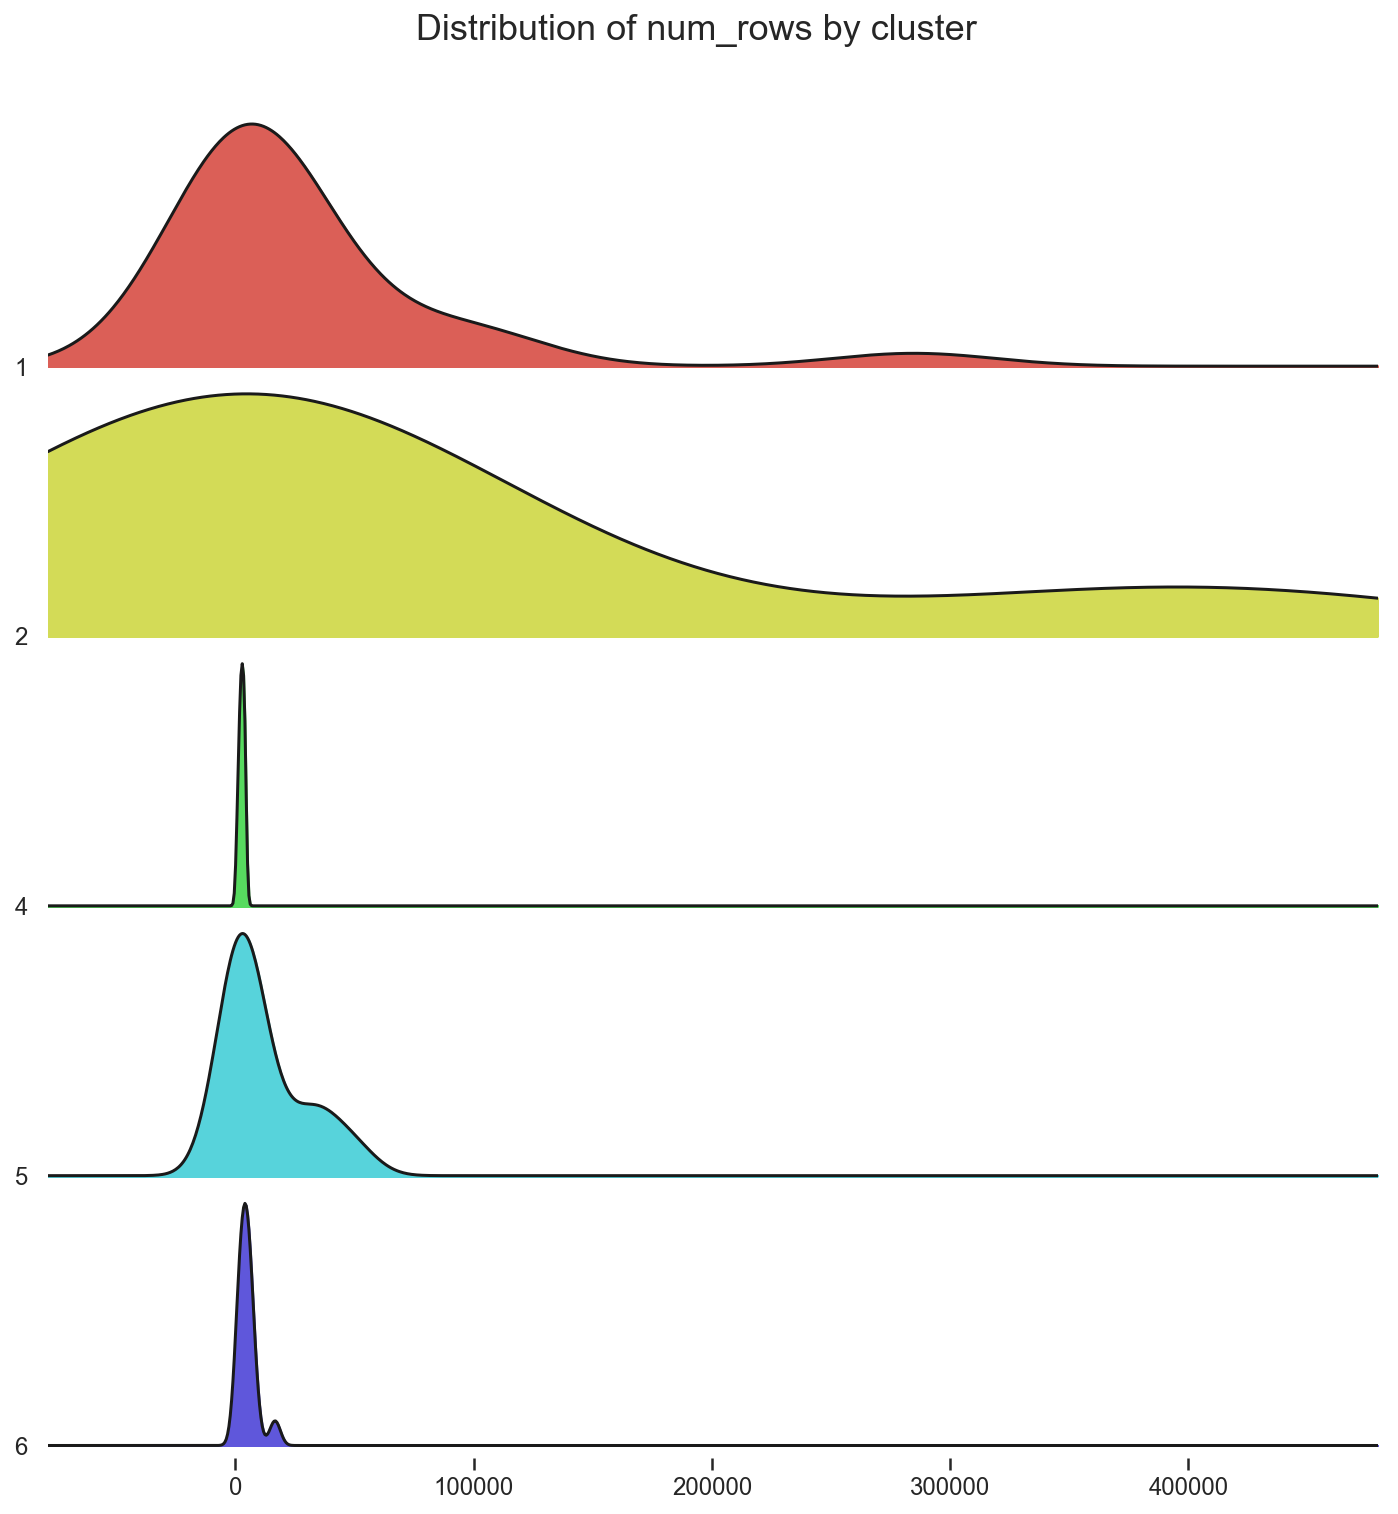
\includegraphics[width=.7\textwidth, height=.7\textwidth]{appendix_figures/joyplot_1.png}
    \caption{Ridgeline plot of \code{num\_rows} }
\end{figure}
\begin{figure}[!ht]
    \centering
    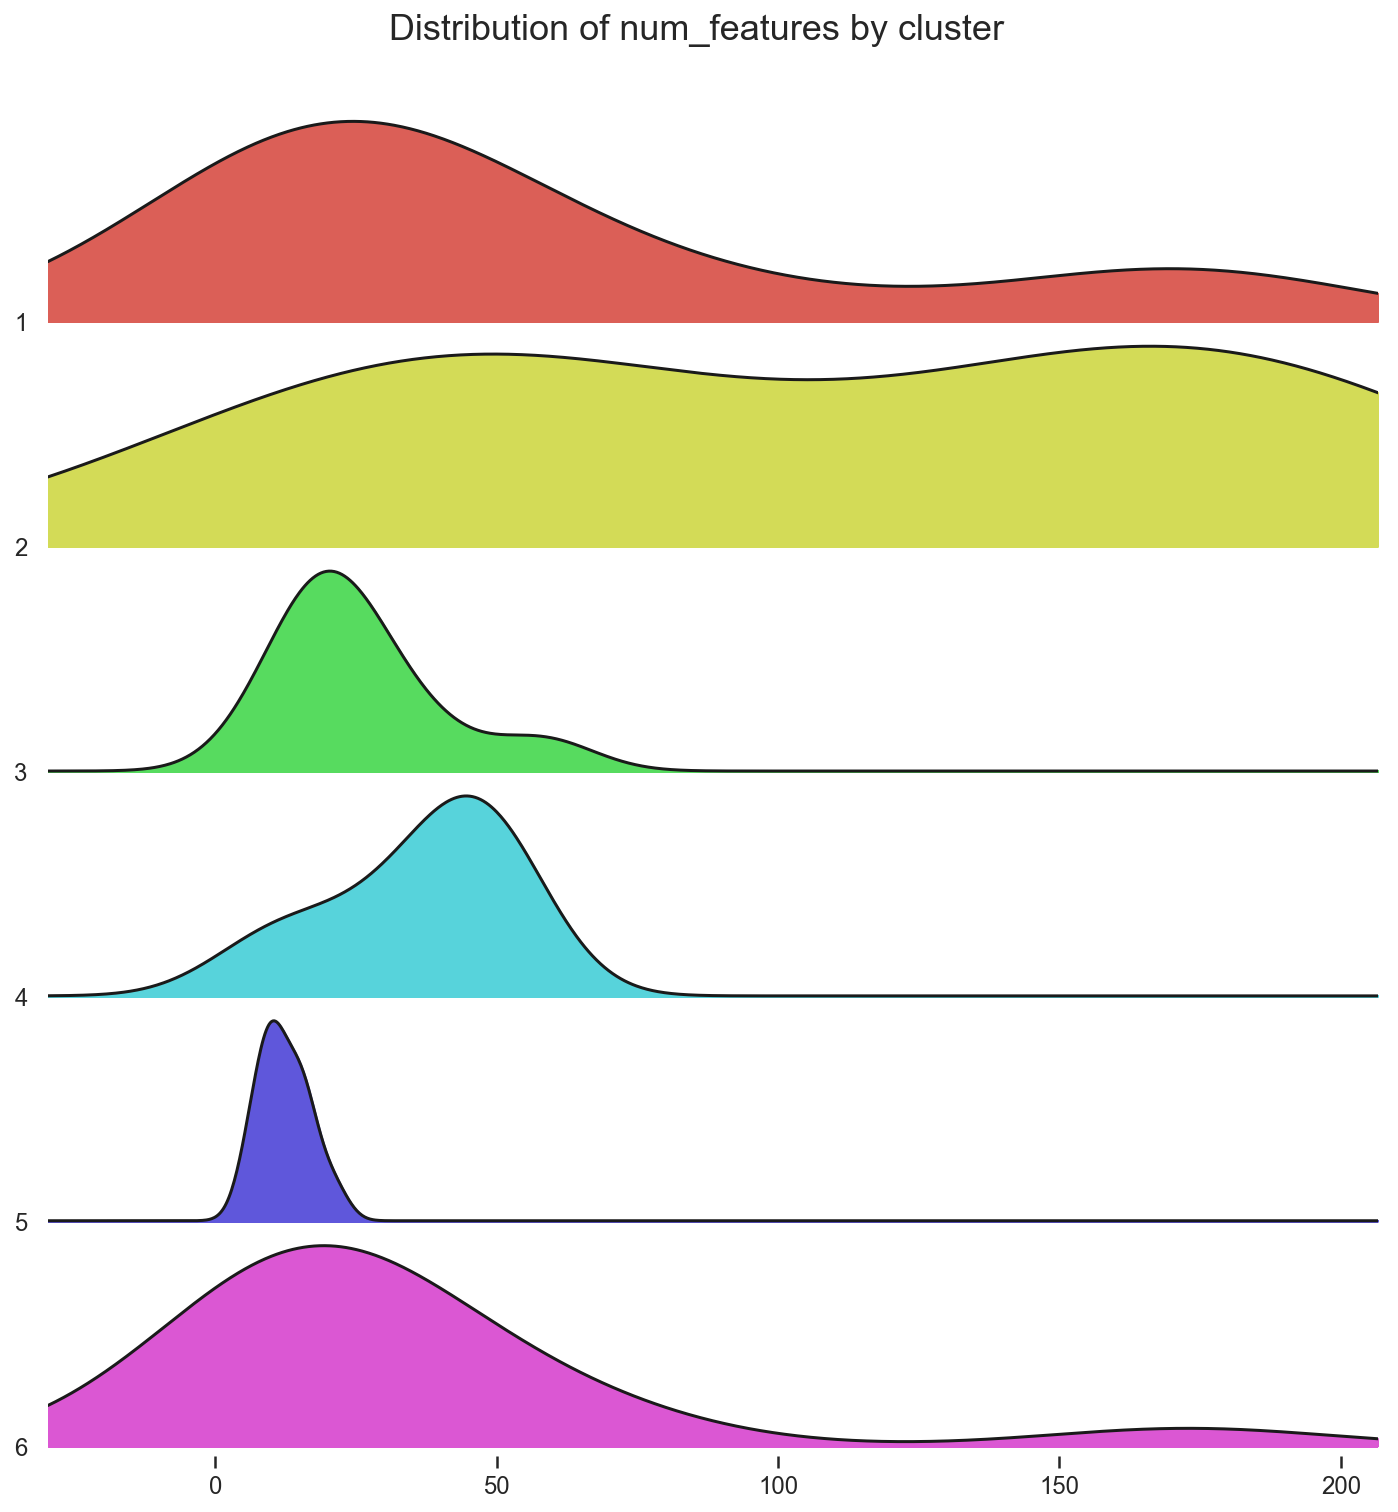
\includegraphics[width=.7\textwidth, height=.7\textwidth]{appendix_figures/joyplot_2.png}
    \caption{Ridgeline plot of \code{num\_features} }
\end{figure}
\begin{figure}[!ht]
    \centering
    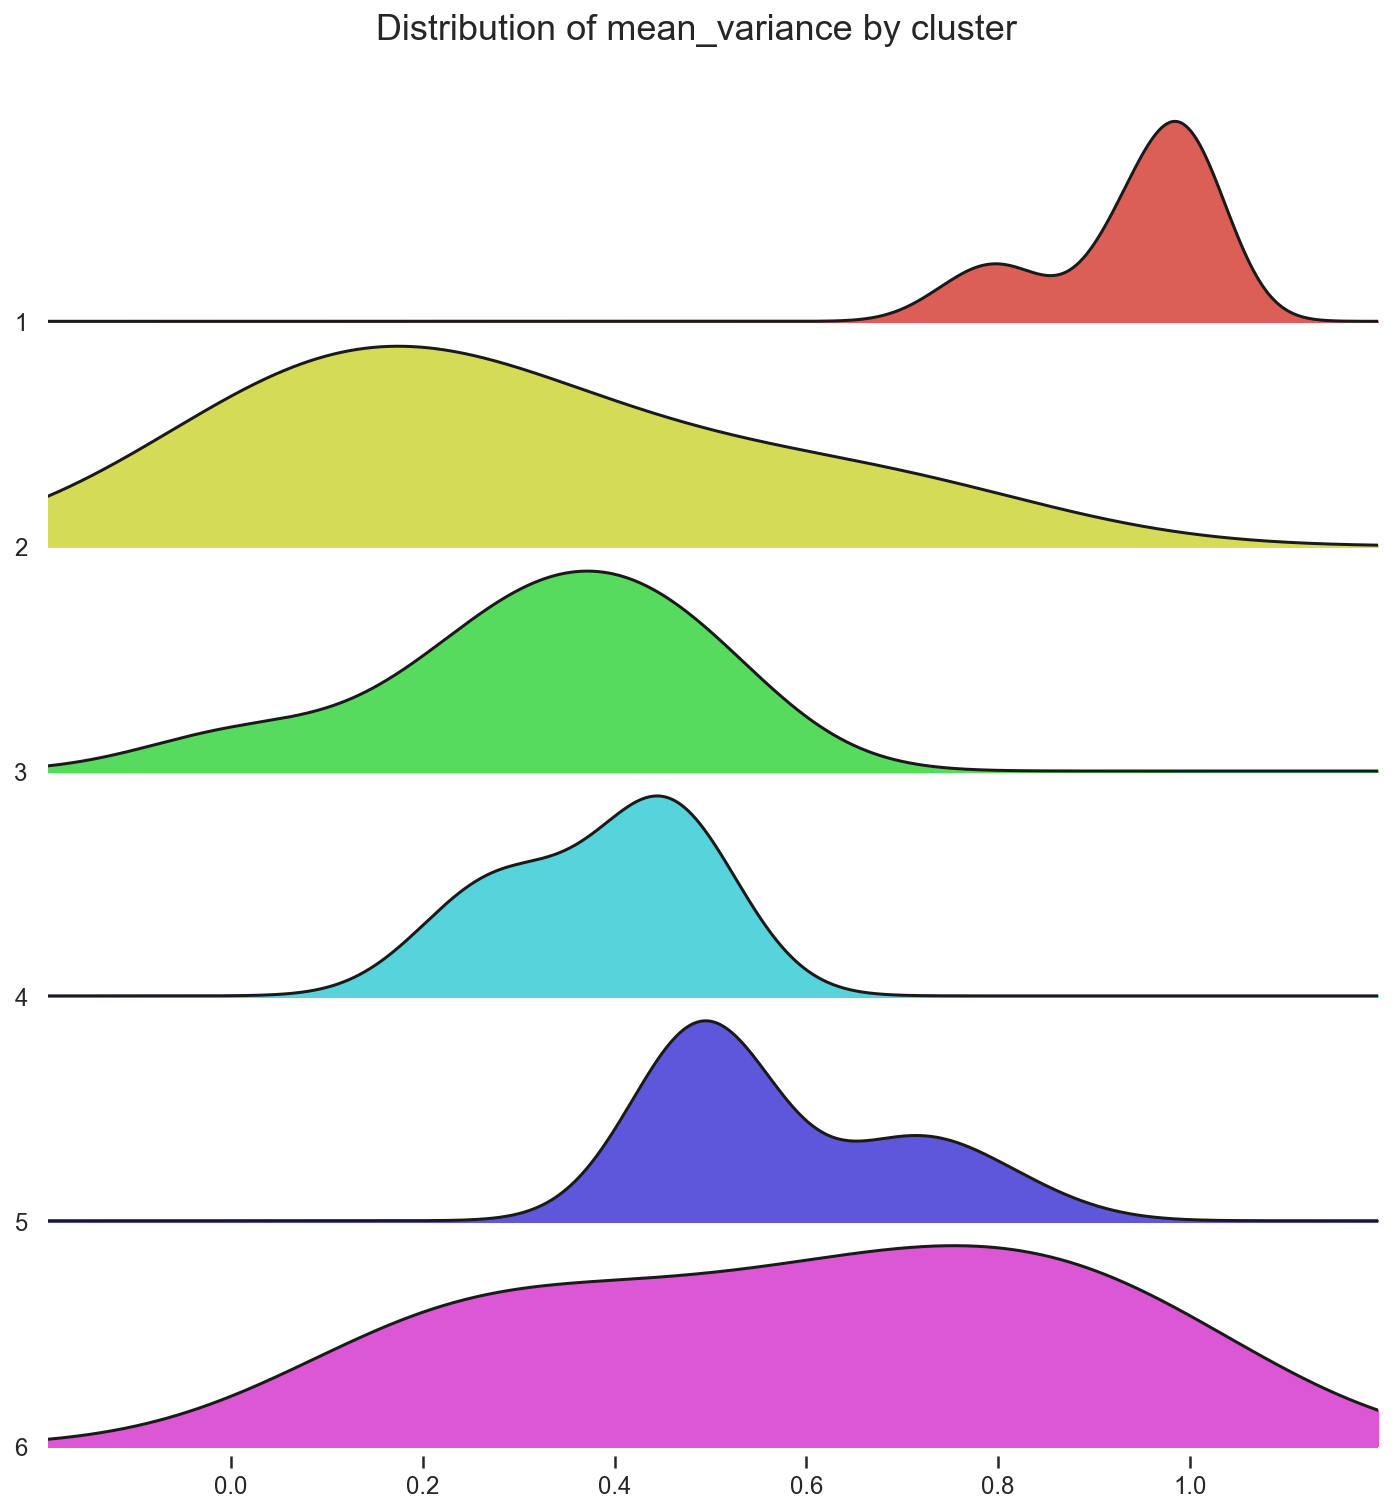
\includegraphics[width=.7\textwidth, height=.7\textwidth]{appendix_figures/joyplot_3.png}
    \caption{Ridgeline plot of \code{mean\_variance} }
\end{figure}
\begin{figure}[!ht]
    \centering
    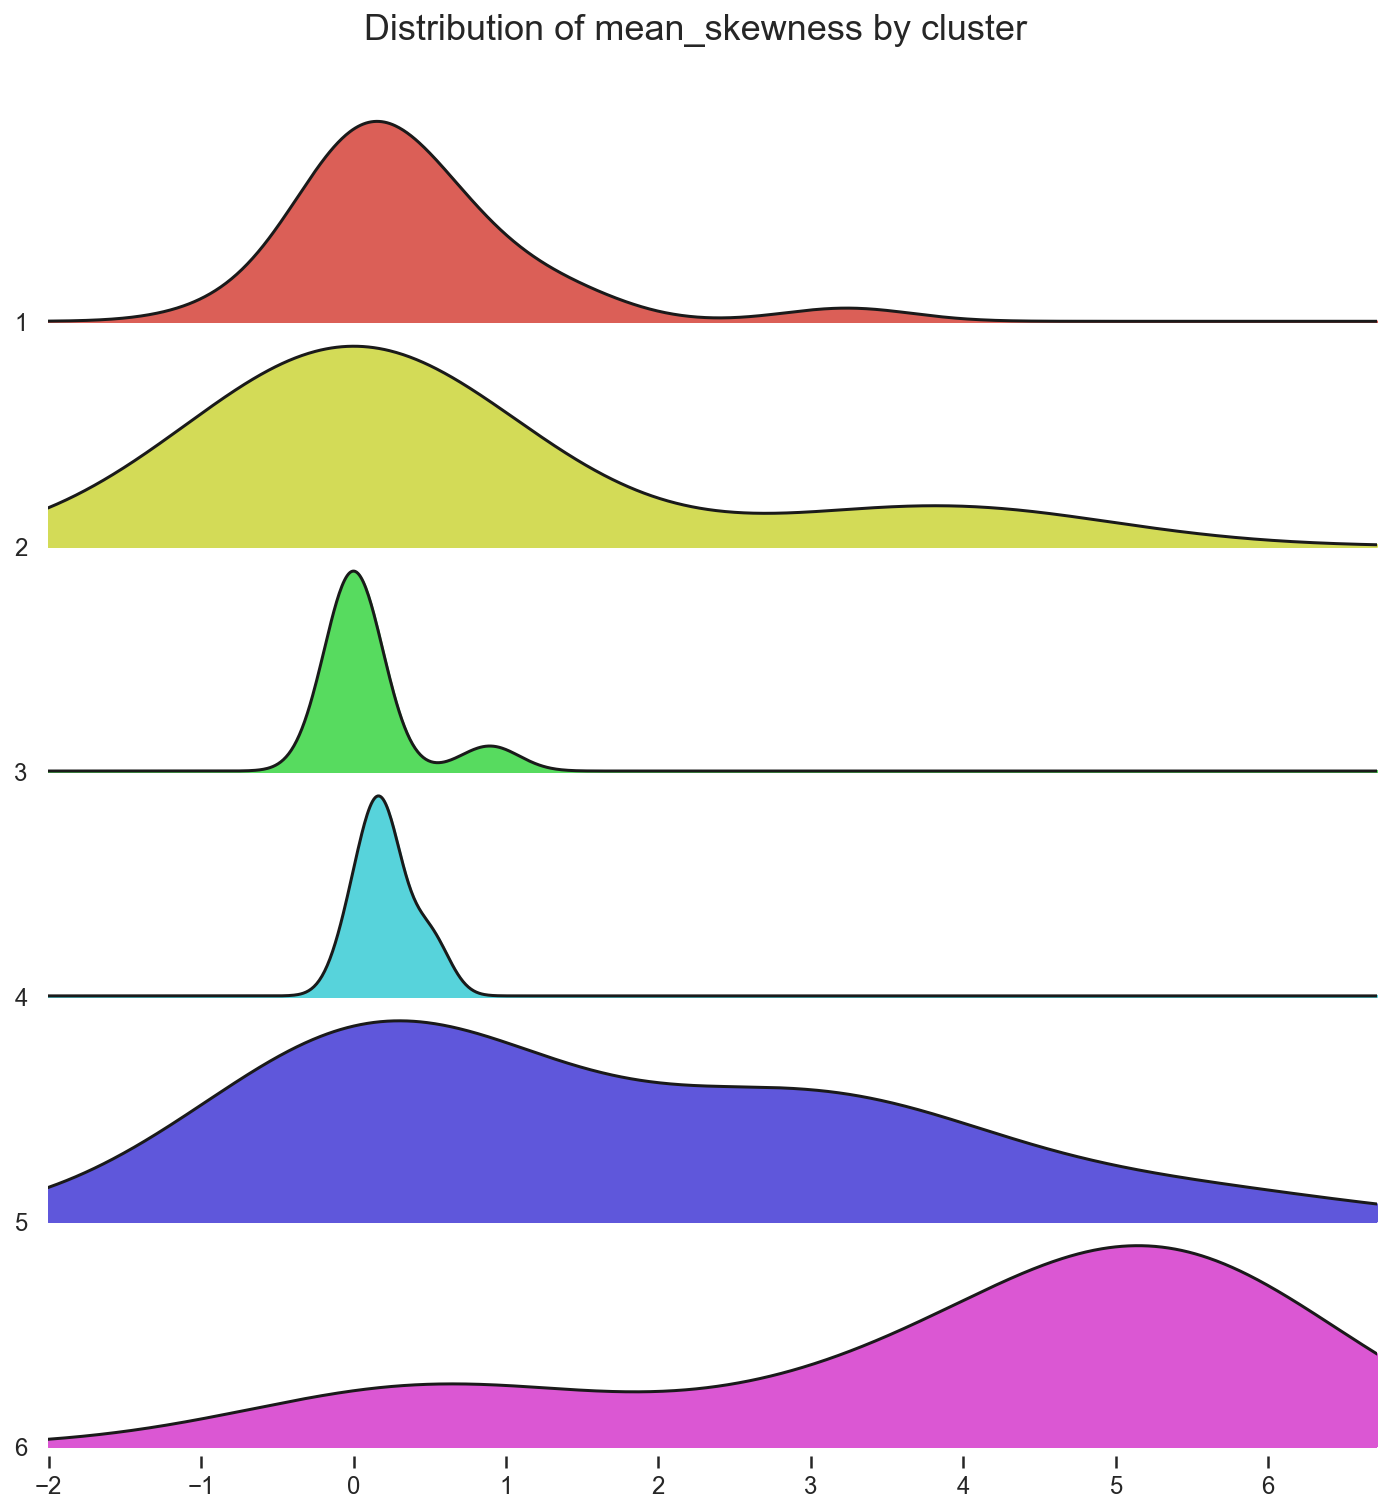
\includegraphics[width=.7\textwidth, height=.7\textwidth]{appendix_figures/joyplot_4.png}
    \caption{Ridgeline plot of \code{mean\_skewness} }
\end{figure}
\begin{figure}[!ht]
    \centering
    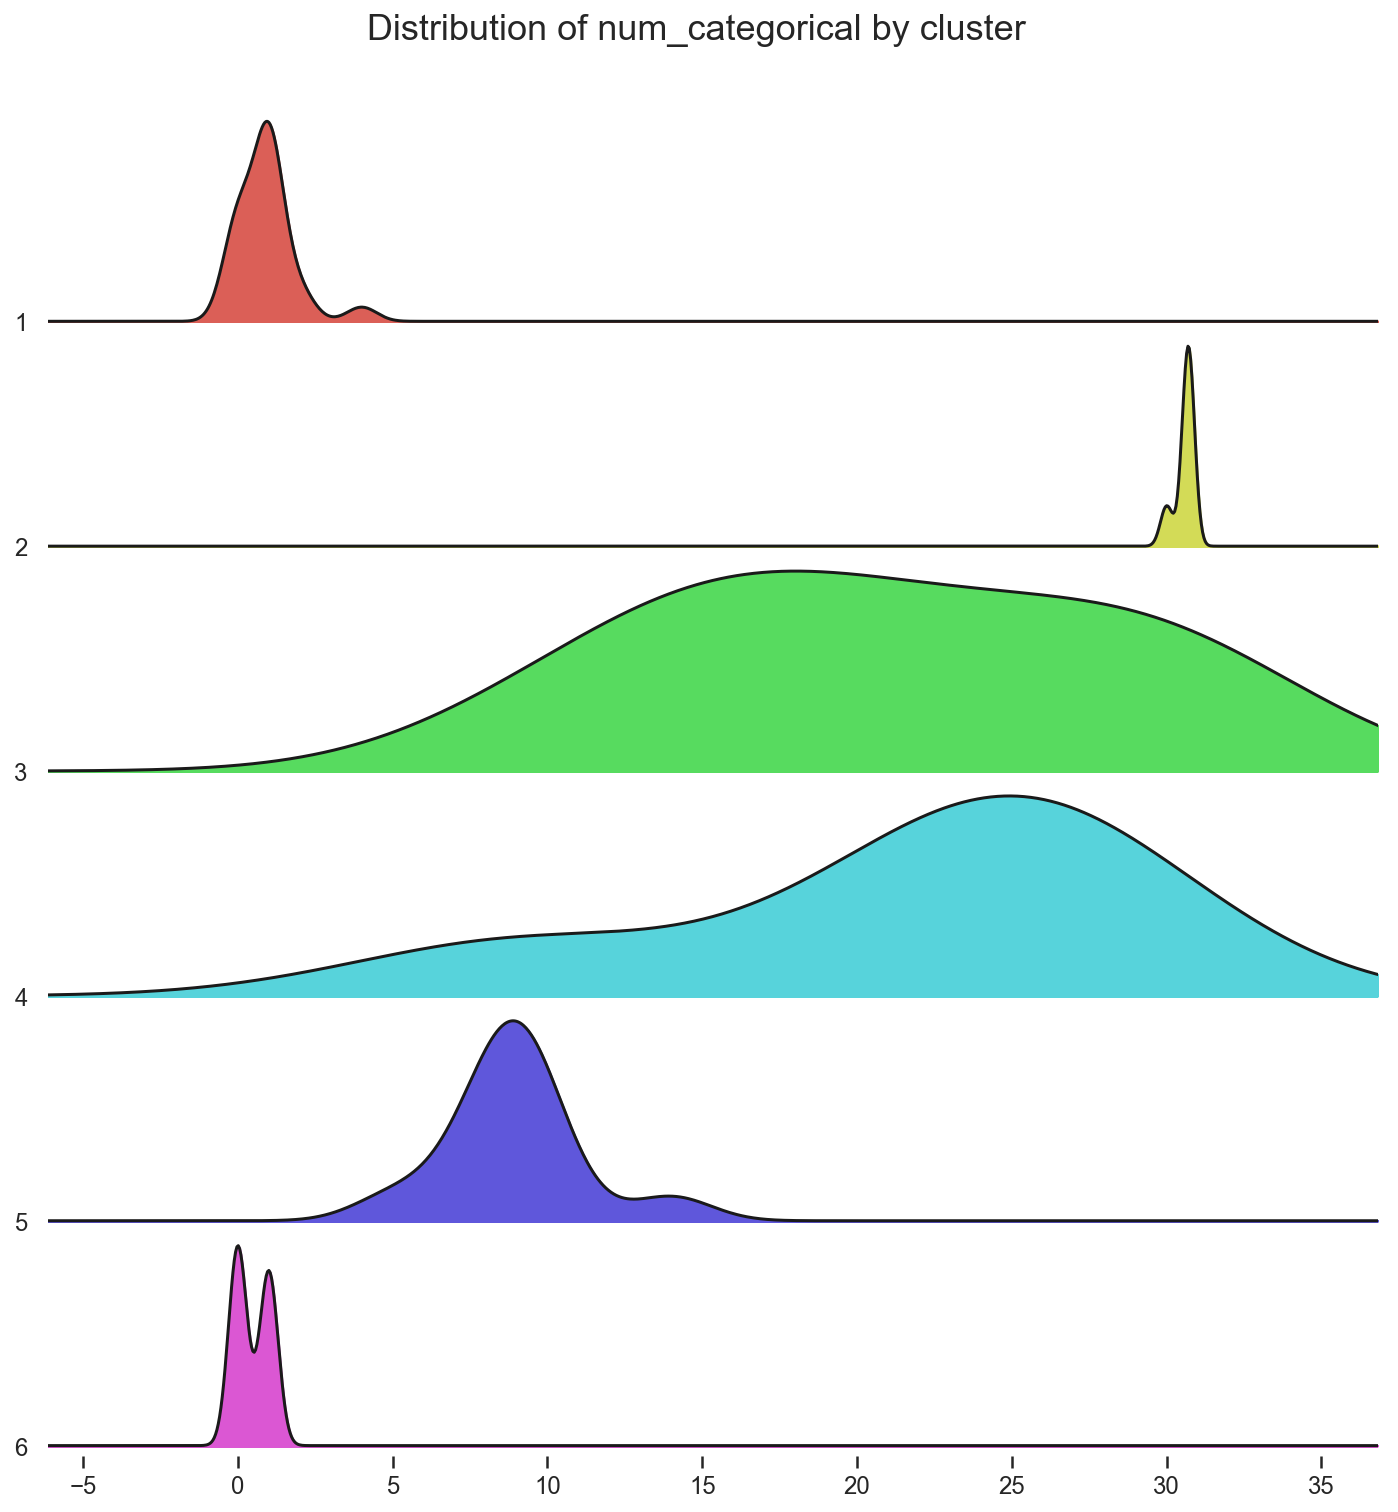
\includegraphics[width=.7\textwidth, height=.7\textwidth]{appendix_figures/joyplot_5.png}
    \caption{Ridgeline plot of \code{num\_categorical} }
\end{figure}
\begin{figure}[!ht]
    \centering
    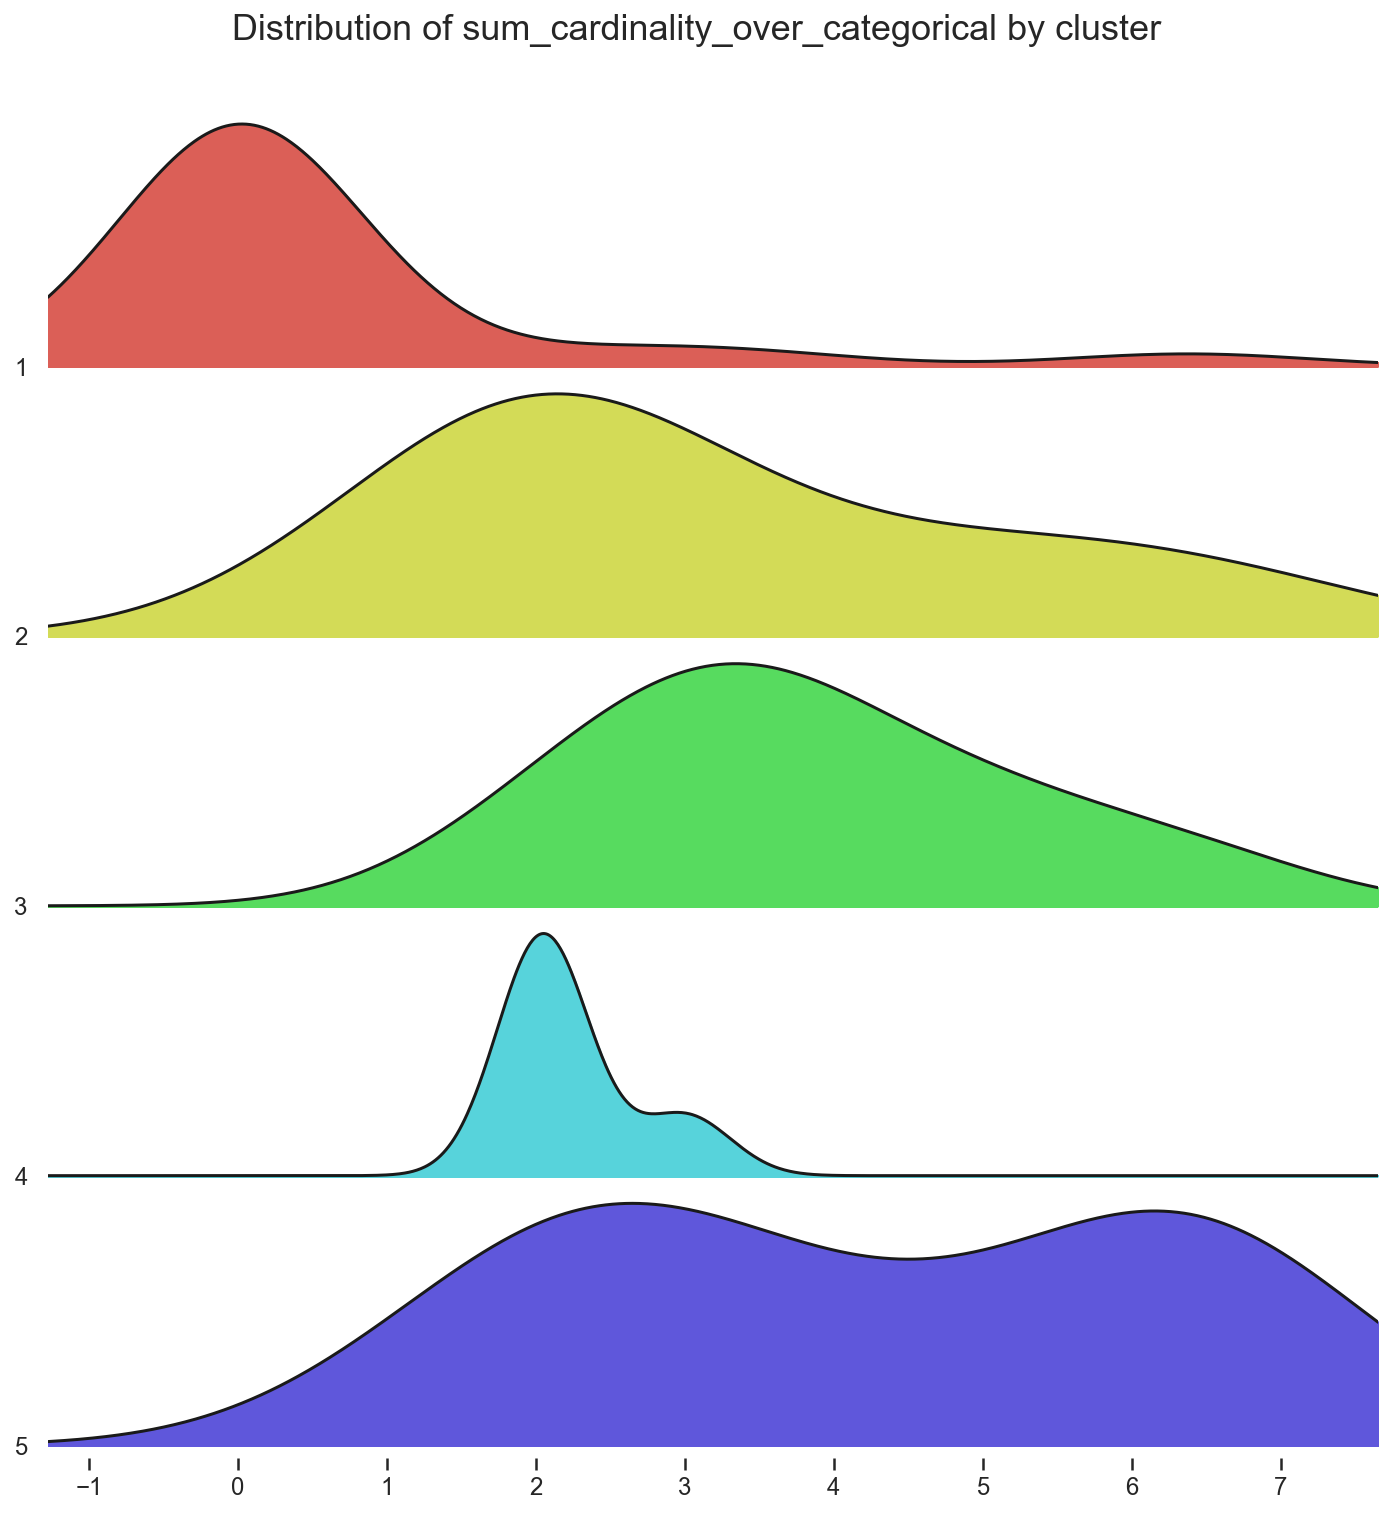
\includegraphics[width=.7\textwidth, height=.7\textwidth]{appendix_figures/joyplot_6.png}
    \caption{Ridgeline plot of \code{sum\_cardinality\_over\_categorical} }
\end{figure}
\begin{figure}[!ht]
    \centering
    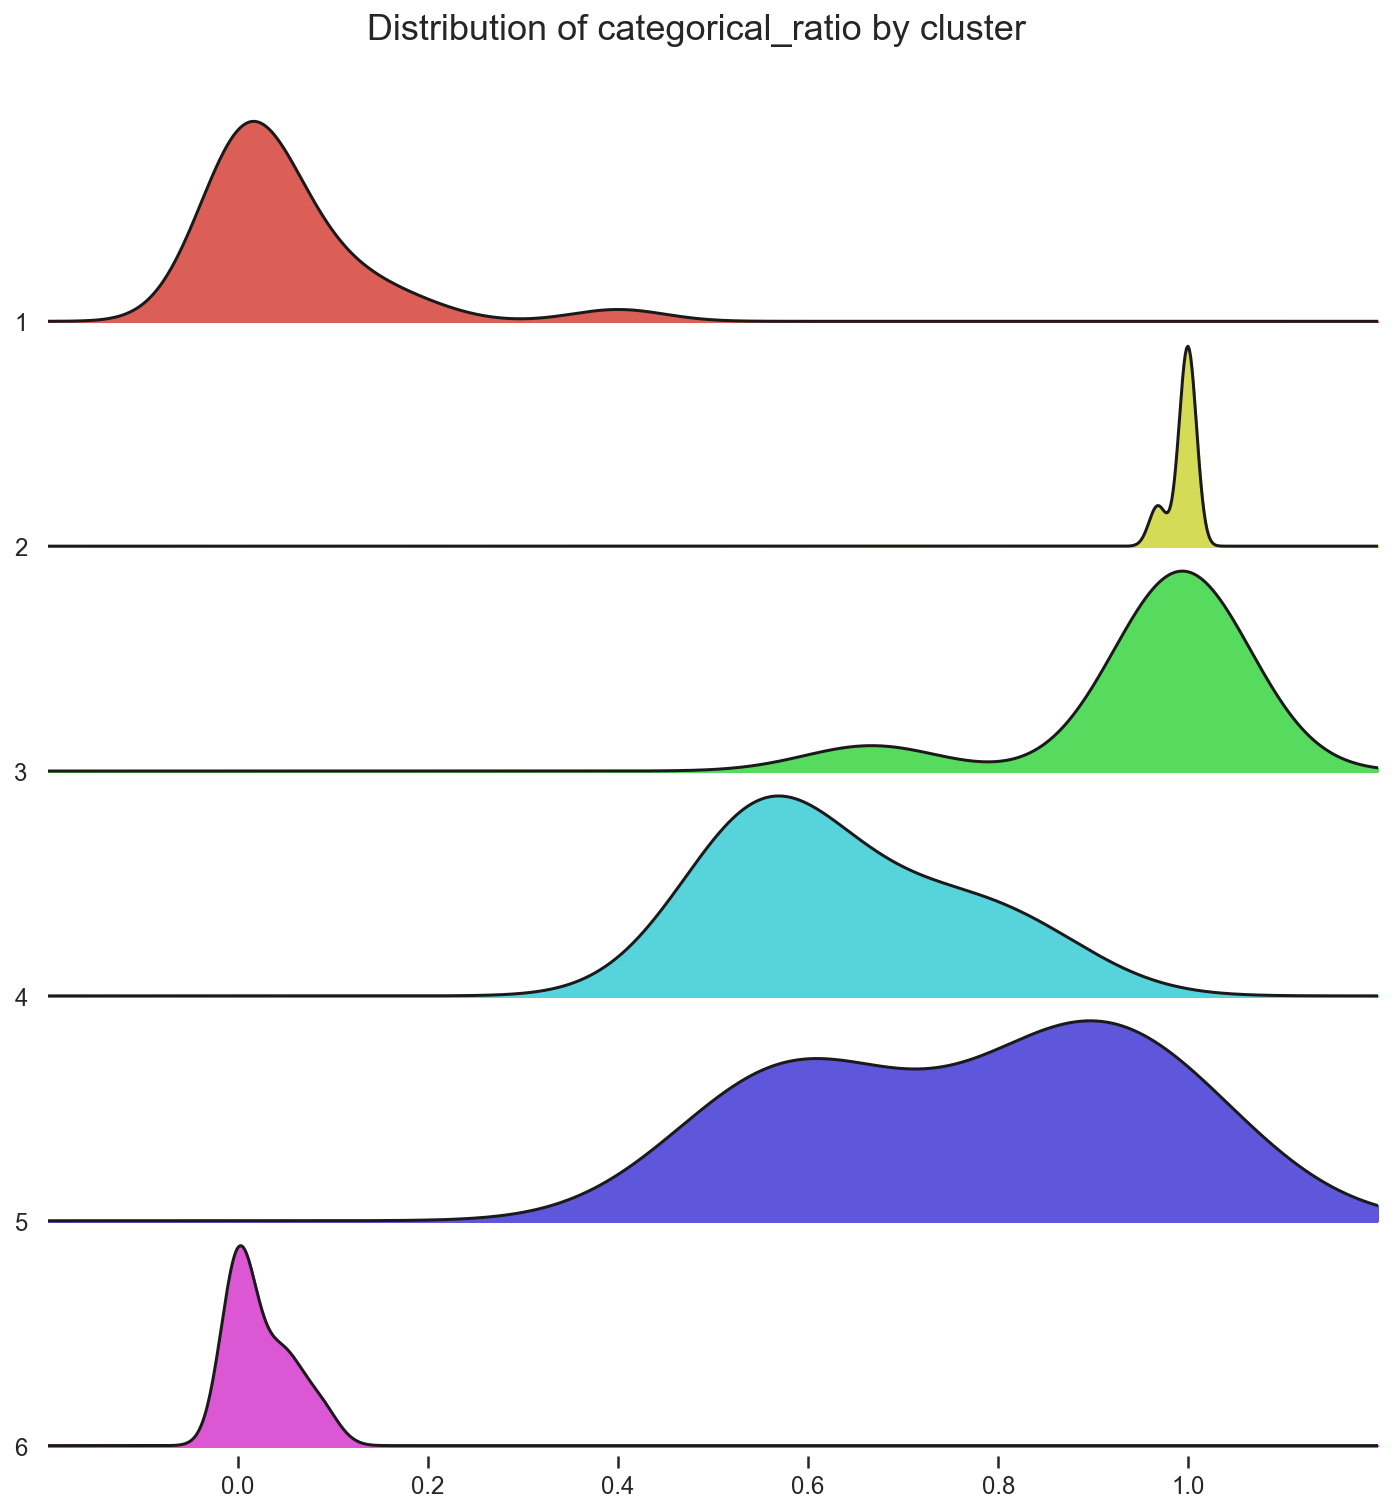
\includegraphics[width=.7\textwidth, height=.7\textwidth]{appendix_figures/joyplot_7.png}
    \caption{Ridgeline plot of \code{categorical\_ratio} }
\end{figure}
\begin{figure}[!ht]
    \centering
    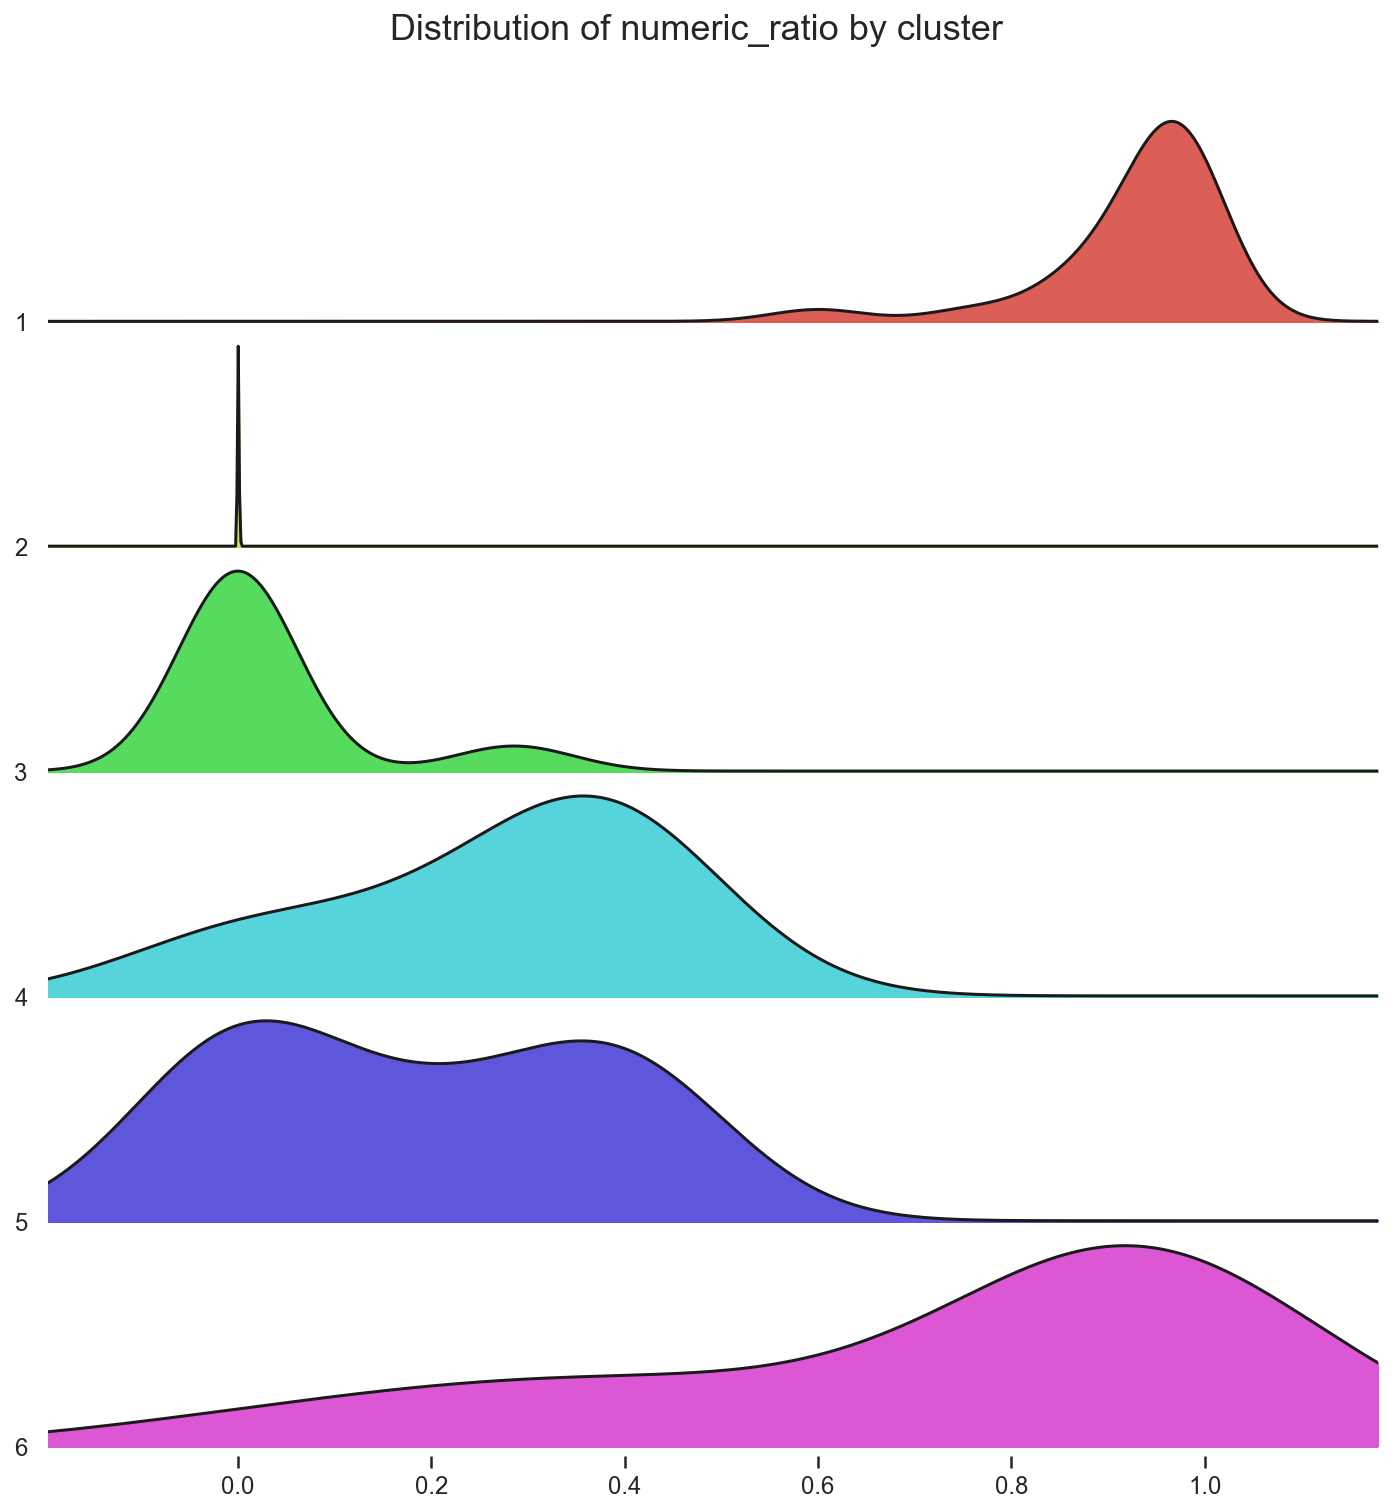
\includegraphics[width=.7\textwidth, height=.7\textwidth]{appendix_figures/joyplot_8.png}
    \caption{Ridgeline plot of \code{numeric\_ratio} }
\end{figure}
\begin{figure}[!ht]
    \centering
    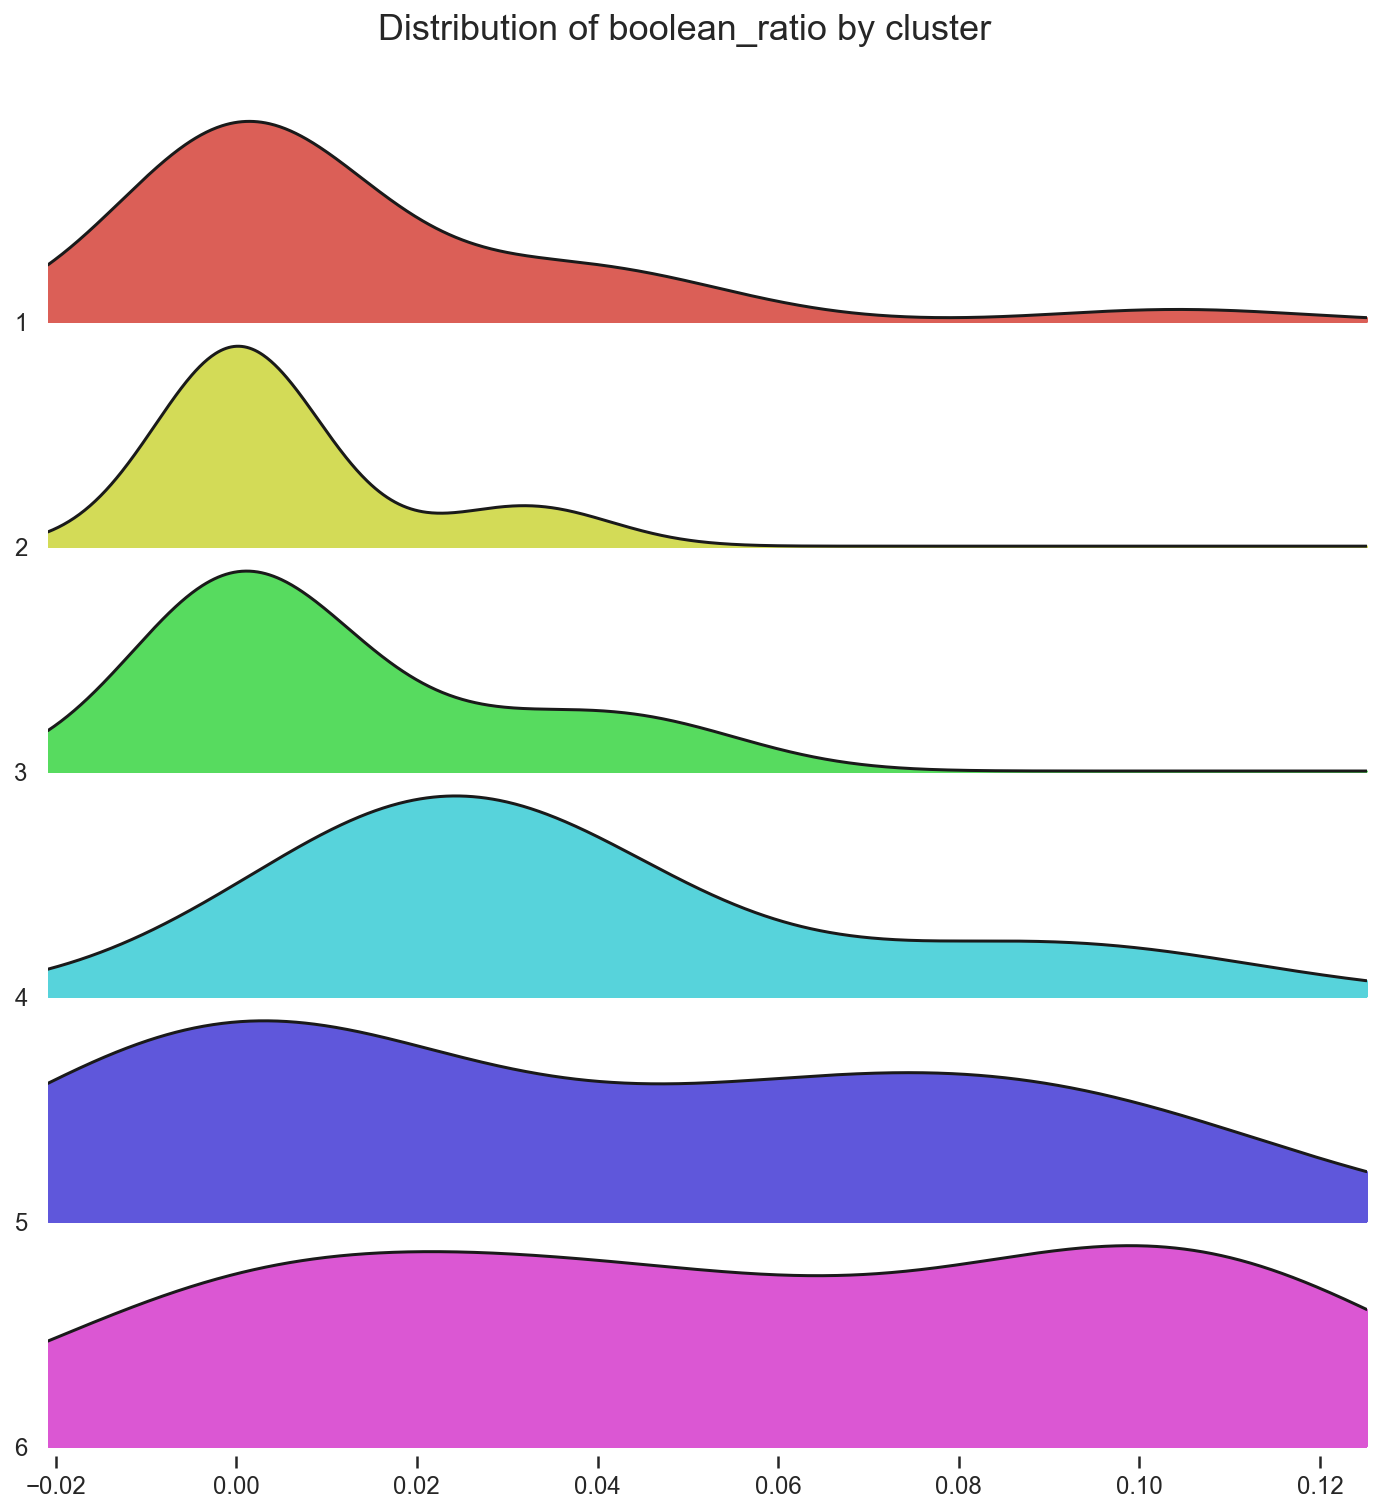
\includegraphics[width=.7\textwidth, height=.7\textwidth]{appendix_figures/joyplot_9.png}
    \caption{Ridgeline plot of \code{boolean\_ratio} }
\end{figure}
\chapter{Statistical Tests Results}
\label{ape:statistical-tests}

\singlespacing

\renewcommand{\arraystretch}{0.85}
\captionsetup{margin=1.0cm}  % correção nas margens dos captions.
%--------------------------------------------------------------------------------------
\begin{table}[!h]
    \centering
    \begin{tabular}{l|lrrr}
    \toprule
                              &                    &  \textbf{Shapiro–Wilk} &  \textbf{Levene} &  \textbf{Kruskal-Wallis} \\
    \textbf{Treatment} & \textbf{Metric} &                        &                  &                          \\
    \midrule
    $\eta^{(1)}_{NE}$ & $\delta_{AUC}$ &           4.965994e-19 &     9.630606e-01 &             9.951832e-01 \\
                              & $\delta_{Brier}$ &           3.710903e-24 &     9.999938e-01 &             9.793033e-01 \\
                              & $\delta_{Logloss}$ &           6.203025e-23 &     9.828542e-01 &             3.733919e-04 \\
    $\eta^{(1)}_{MD}$ & $\delta_{AUC}$ &           3.388219e-21 &     8.590251e-01 &             2.901450e-01 \\
                              & $\delta_{Brier}$ &           8.838670e-15 &     2.941775e-01 &             4.174048e-04 \\
                              & $\delta_{Logloss}$ &           9.113385e-14 &     1.231119e-01 &             1.246510e-02 \\
    $\eta^{(1)}_{LR}$ & $\delta_{AUC}$ &           1.013322e-07 &     9.811205e-01 &             2.878008e-02 \\
                              & $\delta_{Brier}$ &           5.617271e-14 &     1.408917e-03 &             2.329982e-07 \\
                              & $\delta_{Logloss}$ &           7.958839e-14 &     1.050014e-03 &             3.927624e-07 \\
    $\eta^{(1)}_{MD, LR}$ & $\delta_{AUC}$ &           2.401885e-32 &     9.999982e-01 &             6.661712e-08 \\
                              & $\delta_{Brier}$ &           1.177091e-43 &     3.361336e-01 &             1.067366e-90 \\
                              & $\delta_{Logloss}$ &           6.678448e-41 &     9.901324e-19 &             8.193802e-91 \\
    $\eta^{(1)}_{MD, NE}$ & $\delta_{AUC}$ &           0.000000e+00 &     1.000000e+00 &             1.000000e+00 \\
                              & $\delta_{Brier}$ &           0.000000e+00 &     1.000000e+00 &             1.000000e+00 \\
                              & $\delta_{Logloss}$ &           0.000000e+00 &     1.000000e+00 &             1.025601e-04 \\
    $\eta^{(1)}_{LR, NE}$ & $\delta_{AUC}$ &           0.000000e+00 &     6.240957e-01 &             2.852539e-01 \\
                              & $\delta_{Brier}$ &           0.000000e+00 &     9.999999e-01 &             4.590395e-17 \\
                              & $\delta_{Logloss}$ &           0.000000e+00 &     1.000000e+00 &             1.088594e-33 \\
    $\eta^{(1)}_{NE, MD, LR}$ & $\delta_{AUC}$ &           0.000000e+00 &     1.000000e+00 &             1.089024e-10 \\
                              & $\delta_{Brier}$ &           0.000000e+00 &     1.000000e+00 &            6.880061e-293 \\
                              & $\delta_{Logloss}$ &           0.000000e+00 &     1.000000e+00 &             0.000000e+00 \\
    \bottomrule
    \end{tabular}
    \caption{Statistical $p$-values of the experiment scenarios in Cluster 1}
    \end{table}
    
    
    \begin{table}[!h]
    \centering
    \begin{tabular}{l|lrrr}
    \toprule
                              &                    &  \textbf{Shapiro–Wilk} &  \textbf{Levene} &  \textbf{Kruskal-Wallis} \\
    \textbf{Treatment} & \textbf{Metric} &                        &                  &                          \\
    \midrule
    $\eta^{(2)}_{NE}$ & $\delta_{AUC}$ &           4.059920e-08 &     9.968117e-01 &             9.996506e-01 \\
                              & $\delta_{Brier}$ &           5.942564e-06 &     2.105453e-01 &             9.965572e-01 \\
                              & $\delta_{Logloss}$ &           2.502680e-05 &     9.636175e-03 &             2.827828e-03 \\
    $\eta^{(2)}_{MD}$ & $\delta_{AUC}$ &           2.536182e-10 &     9.210022e-01 &             1.860650e-02 \\
                              & $\delta_{Brier}$ &           3.926061e-06 &     2.774635e-01 &             2.283747e-02 \\
                              & $\delta_{Logloss}$ &           2.522154e-05 &     1.285176e-01 &             1.764531e-02 \\
    $\eta^{(2)}_{LR}$ & $\delta_{AUC}$ &           2.714980e-09 &              NaN &                      NaN \\
                              & $\delta_{Brier}$ &           9.808685e-09 &              NaN &                      NaN \\
                              & $\delta_{Logloss}$ &           1.213540e-10 &              NaN &                      NaN \\
    $\eta^{(2)}_{MD, LR}$ & $\delta_{AUC}$ &           1.406702e-20 &     9.999939e-01 &             1.316980e-02 \\
                              & $\delta_{Brier}$ &           1.339994e-23 &     1.000000e+00 &             6.235464e-12 \\
                              & $\delta_{Logloss}$ &           1.334960e-23 &     1.000000e+00 &             1.005025e-08 \\
    $\eta^{(2)}_{MD, NE}$ & $\delta_{AUC}$ &           2.548462e-22 &     1.000000e+00 &             1.000000e+00 \\
                              & $\delta_{Brier}$ &           6.494320e-28 &     9.969882e-01 &             9.274816e-01 \\
                              & $\delta_{Logloss}$ &           3.974093e-21 &     2.655356e-23 &             6.191510e-22 \\
    $\eta^{(2)}_{LR, NE}$ & $\delta_{AUC}$ &           9.960932e-27 &     1.000000e+00 &             3.306332e-06 \\
                              & $\delta_{Brier}$ &           2.709085e-26 &     9.999995e-01 &             7.035798e-09 \\
                              & $\delta_{Logloss}$ &           2.452305e-24 &     9.999999e-01 &             1.650304e-05 \\
    $\eta^{(2)}_{NE, MD, LR}$ & $\delta_{AUC}$ &           0.000000e+00 &     1.000000e+00 &             2.904172e-64 \\
                              & $\delta_{Brier}$ &           0.000000e+00 &     1.000000e+00 &            4.013155e-111 \\
                              & $\delta_{Logloss}$ &           0.000000e+00 &     1.000000e+00 &             7.298816e-70 \\
    \bottomrule
    \end{tabular}
    \caption{Statistical $p$-values of the experiment scenarios in Cluster 2}
    \end{table}
    
    
    \begin{table}[!h]
    \centering
    \begin{tabular}{l|lrrr}
    \toprule
                              &                    &  \textbf{Shapiro–Wilk} &  \textbf{Levene} &  \textbf{Kruskal-Wallis} \\
    \textbf{Treatment} & \textbf{Metric} &                        &                  &                          \\
    \midrule
    $\eta^{(3)}_{NE}$ & $\delta_{AUC}$ &           5.611898e-16 &     9.988256e-01 &             1.147338e-01 \\
                              & $\delta_{Brier}$ &           2.050222e-10 &     8.124238e-01 &             9.418066e-02 \\
                              & $\delta_{Logloss}$ &           8.273422e-11 &     6.302806e-01 &             2.663393e-01 \\
    $\eta^{(3)}_{MD}$ & $\delta_{AUC}$ &           3.139396e-07 &     2.645190e-02 &             2.556998e-05 \\
                              & $\delta_{Brier}$ &           3.959432e-05 &     3.419306e-02 &             4.180864e-06 \\
                              & $\delta_{Logloss}$ &           6.005177e-04 &     3.551900e-02 &             2.702174e-06 \\
    $\eta^{(3)}_{LR}$ & $\delta_{AUC}$ &           3.676430e-01 &     1.621118e-01 &             1.767196e-06 \\
                              & $\delta_{Brier}$ &           5.871765e-03 &     6.829990e-04 &             1.551529e-06 \\
                              & $\delta_{Logloss}$ &           1.938849e-02 &     6.932106e-06 &             1.598158e-06 \\
    $\eta^{(3)}_{MD, LR}$ & $\delta_{AUC}$ &           8.839741e-14 &     5.496276e-01 &             2.534254e-20 \\
                              & $\delta_{Brier}$ &           5.927692e-07 &     7.132355e-01 &             8.655283e-48 \\
                              & $\delta_{Logloss}$ &           3.870745e-10 &     3.646846e-02 &             1.441531e-51 \\
    $\eta^{(3)}_{MD, NE}$ & $\delta_{AUC}$ &           3.996994e-40 &     3.524884e-03 &             6.177612e-25 \\
                              & $\delta_{Brier}$ &           2.490148e-35 &     2.958452e-02 &             6.911108e-22 \\
                              & $\delta_{Logloss}$ &           2.679125e-35 &    1.031149e-169 &            3.001168e-100 \\
    $\eta^{(3)}_{LR, NE}$ & $\delta_{AUC}$ &           8.223911e-28 &     3.639094e-15 &             4.084732e-19 \\
                              & $\delta_{Brier}$ &           4.965566e-27 &     1.425324e-08 &             6.548453e-23 \\
                              & $\delta_{Logloss}$ &           1.446958e-34 &     5.364655e-11 &             1.063454e-24 \\
    $\eta^{(3)}_{NE, MD, LR}$ & $\delta_{AUC}$ &           0.000000e+00 &     2.067193e-23 &            2.847486e-123 \\
                              & $\delta_{Brier}$ &           1.401298e-45 &     1.522520e-09 &            1.016972e-125 \\
                              & $\delta_{Logloss}$ &           1.401298e-45 &     0.000000e+00 &             0.000000e+00 \\
    \bottomrule
    \end{tabular}
    \caption{Statistical $p$-values of the experiment scenarios in Cluster 3}
    \end{table}
    
    
    \begin{table}[!h]
    \centering
    \begin{tabular}{l|lrrr}
    \toprule
                              &                    &  \textbf{Shapiro–Wilk} &  \textbf{Levene} &  \textbf{Kruskal-Wallis} \\
    \textbf{Treatment} & \textbf{Metric} &                        &                  &                          \\
    \midrule
    $\eta^{(4)}_{NE}$ & $\delta_{AUC}$ &           3.616501e-13 &     9.873830e-01 &             2.111212e-01 \\
                              & $\delta_{Brier}$ &           2.482372e-13 &     9.980555e-01 &             9.970748e-01 \\
                              & $\delta_{Logloss}$ &           1.336703e-11 &     9.292868e-01 &             9.770873e-01 \\
    $\eta^{(4)}_{MD}$ & $\delta_{AUC}$ &           2.537239e-11 &     9.982780e-01 &             9.797863e-01 \\
                              & $\delta_{Brier}$ &           1.019241e-06 &     9.964629e-01 &             9.957778e-01 \\
                              & $\delta_{Logloss}$ &           6.850468e-10 &     9.998679e-01 &             9.999136e-01 \\
    $\eta^{(4)}_{LR}$ & $\delta_{AUC}$ &           1.831653e-07 &     0.000000e+00 &             1.000000e+00 \\
                              & $\delta_{Brier}$ &           3.636517e-09 &     0.000000e+00 &             1.024704e-01 \\
                              & $\delta_{Logloss}$ &           3.636517e-09 &     6.581044e-29 &             1.024704e-01 \\
    $\eta^{(4)}_{MD, LR}$ & $\delta_{AUC}$ &           9.831066e-33 &     9.999617e-01 &             7.098868e-01 \\
                              & $\delta_{Brier}$ &           9.176373e-28 &     1.000000e+00 &             2.899170e-10 \\
                              & $\delta_{Logloss}$ &           2.758601e-30 &     9.999158e-01 &             5.548296e-09 \\
    $\eta^{(4)}_{MD, NE}$ & $\delta_{AUC}$ &           3.372529e-39 &     1.000000e+00 &             9.862816e-01 \\
                              & $\delta_{Brier}$ &           0.000000e+00 &     1.000000e+00 &             1.000000e+00 \\
                              & $\delta_{Logloss}$ &           4.203895e-45 &     1.000000e+00 &             1.000000e+00 \\
    $\eta^{(4)}_{LR, NE}$ & $\delta_{AUC}$ &           1.439362e-30 &     9.994980e-01 &             1.000000e+00 \\
                              & $\delta_{Brier}$ &           1.217919e-29 &     9.984107e-01 &             1.066378e-08 \\
                              & $\delta_{Logloss}$ &           2.404549e-26 &     9.772312e-01 &             4.468989e-09 \\
    $\eta^{(4)}_{NE, MD, LR}$ & $\delta_{AUC}$ &           0.000000e+00 &     1.000000e+00 &             1.000000e+00 \\
                              & $\delta_{Brier}$ &           0.000000e+00 &     1.000000e+00 &            2.812655e-136 \\
                              & $\delta_{Logloss}$ &           0.000000e+00 &     1.000000e+00 &            2.501047e-153 \\
    \bottomrule
    \end{tabular}
    \caption{Statistical $p$-values of the experiment scenarios in Cluster 4}
    \end{table}
    
    
    \begin{table}[!h]
    \centering
    \begin{tabular}{l|lrrr}
    \toprule
                              &                    &  \textbf{Shapiro–Wilk} &  \textbf{Levene} &  \textbf{Kruskal-Wallis} \\
    \textbf{Treatment} & \textbf{Metric} &                        &                  &                          \\
    \midrule
    $\eta^{(5)}_{NE}$ & $\delta_{AUC}$ &           2.727656e-13 &     9.999921e-01 &             8.138489e-01 \\
                              & $\delta_{Brier}$ &           2.316378e-11 &     5.085153e-01 &             9.999896e-01 \\
                              & $\delta_{Logloss}$ &           5.203110e-10 &     5.821598e-03 &             9.999997e-01 \\
    $\eta^{(5)}_{MD}$ & $\delta_{AUC}$ &           1.056675e-27 &     9.999371e-01 &             3.299262e-01 \\
                              & $\delta_{Brier}$ &           5.635529e-28 &     9.999508e-01 &             1.229116e-04 \\
                              & $\delta_{Logloss}$ &           1.100347e-27 &     9.999037e-01 &             1.275362e-02 \\
    $\eta^{(5)}_{LR}$ & $\delta_{AUC}$ &           6.518040e-13 &     9.998573e-01 &             1.734229e-02 \\
                              & $\delta_{Brier}$ &           3.448695e-14 &     9.983008e-01 &             1.984047e-03 \\
                              & $\delta_{Logloss}$ &           1.160934e-13 &     9.997163e-01 &             2.143289e-03 \\
    $\eta^{(5)}_{MD, LR}$ & $\delta_{AUC}$ &           2.371575e-30 &     1.000000e+00 &             3.281449e-28 \\
                              & $\delta_{Brier}$ &           1.079978e-39 &     1.000000e+00 &             7.005511e-07 \\
                              & $\delta_{Logloss}$ &           3.393346e-36 &     1.000000e+00 &             1.115711e-06 \\
    $\eta^{(5)}_{MD, NE}$ & $\delta_{AUC}$ &           0.000000e+00 &     1.000000e+00 &             1.000000e+00 \\
                              & $\delta_{Brier}$ &           2.802597e-45 &     9.981370e-01 &             1.000000e+00 \\
                              & $\delta_{Logloss}$ &           4.049753e-43 &     6.341819e-85 &             1.000000e+00 \\
    $\eta^{(5)}_{LR, NE}$ & $\delta_{AUC}$ &           0.000000e+00 &     1.000000e+00 &             1.663213e-08 \\
                              & $\delta_{Brier}$ &           0.000000e+00 &     1.000000e+00 &             7.634533e-16 \\
                              & $\delta_{Logloss}$ &           1.401298e-45 &     1.000000e+00 &             1.683672e-15 \\
    $\eta^{(5)}_{NE, MD, LR}$ & $\delta_{AUC}$ &           0.000000e+00 &     1.000000e+00 &             1.252096e-92 \\
                              & $\delta_{Brier}$ &           0.000000e+00 &     1.000000e+00 &            1.095053e-251 \\
                              & $\delta_{Logloss}$ &           0.000000e+00 &     1.000000e+00 &            8.787394e-273 \\
    \bottomrule
    \end{tabular}
    \caption{Statistical $p$-values of the experiment scenarios in Cluster 5}
    \end{table}
    
    
    \begin{table}[!h]
    \centering
    \begin{tabular}{l|lrrr}
    \toprule
                              &                    &  \textbf{Shapiro–Wilk} &  \textbf{Levene} &  \textbf{Kruskal-Wallis} \\
    \textbf{Treatment} & \textbf{Metric} &                        &                  &                          \\
    \midrule
    $\eta^{(6)}_{NE}$ & $\delta_{AUC}$ &           5.555299e-15 &     7.331148e-02 &             9.810169e-05 \\
                              & $\delta_{Brier}$ &           4.446020e-13 &     1.695424e-02 &             1.426687e-07 \\
                              & $\delta_{Logloss}$ &           5.699214e-15 &     1.302647e-04 &             1.309669e-17 \\
    $\eta^{(6)}_{MD}$ & $\delta_{AUC}$ &           8.323186e-18 &     9.659329e-01 &             2.275562e-01 \\
                              & $\delta_{Brier}$ &           8.587676e-18 &     8.808170e-01 &             3.733077e-02 \\
                              & $\delta_{Logloss}$ &           8.382108e-16 &     7.293658e-01 &             1.738130e-01 \\
    $\eta^{(6)}_{LR}$ & $\delta_{AUC}$ &           8.634467e-17 &              NaN &                      NaN \\
                              & $\delta_{Brier}$ &           1.000000e+00 &              NaN &                      NaN \\
                              & $\delta_{Logloss}$ &           5.394157e-16 &              NaN &                      NaN \\
    $\eta^{(6)}_{MD, LR}$ & $\delta_{AUC}$ &           8.691273e-41 &     9.990496e-01 &             3.351863e-04 \\
                              & $\delta_{Brier}$ &           7.470919e-39 &     1.000000e+00 &             6.020948e-12 \\
                              & $\delta_{Logloss}$ &           1.597480e-43 &     9.999978e-01 &             1.947958e-15 \\
    $\eta^{(6)}_{MD, NE}$ & $\delta_{AUC}$ &           0.000000e+00 &     6.248752e-01 &             9.997299e-01 \\
                              & $\delta_{Brier}$ &           6.459986e-43 &     9.233229e-71 &             1.014506e-50 \\
                              & $\delta_{Logloss}$ &           0.000000e+00 &    3.935870e-148 &            5.383524e-198 \\
    $\eta^{(6)}_{LR, NE}$ & $\delta_{AUC}$ &           1.401298e-45 &     9.999975e-01 &             2.575427e-03 \\
                              & $\delta_{Brier}$ &           1.916556e-41 &     2.863830e-01 &             1.070646e-03 \\
                              & $\delta_{Logloss}$ &           0.000000e+00 &     6.187968e-16 &             2.237852e-06 \\
    $\eta^{(6)}_{NE, MD, LR}$ & $\delta_{AUC}$ &           0.000000e+00 &     1.000000e+00 &            2.705704e-150 \\
                              & $\delta_{Brier}$ &           0.000000e+00 &     5.205595e-22 &             6.798990e-02 \\
                              & $\delta_{Logloss}$ &           0.000000e+00 &     0.000000e+00 &             6.851411e-86 \\
    \bottomrule
    \end{tabular}
    \caption{Statistical $p$-values of the experiment scenarios in Cluster 6}
    \end{table}

% \chapter{SFM plots}
\label{ape:sfm-plots}

All the generated SFM plots are illustrated below, for all the experimental scenarios of the study.

\singlespacing

\renewcommand{\arraystretch}{0.85}
\captionsetup{margin=1.0cm}  % correção nas margens dos captions.
%--------------------------------------------------------------------------------------


\begin{figure}[!ht]
    \centering
    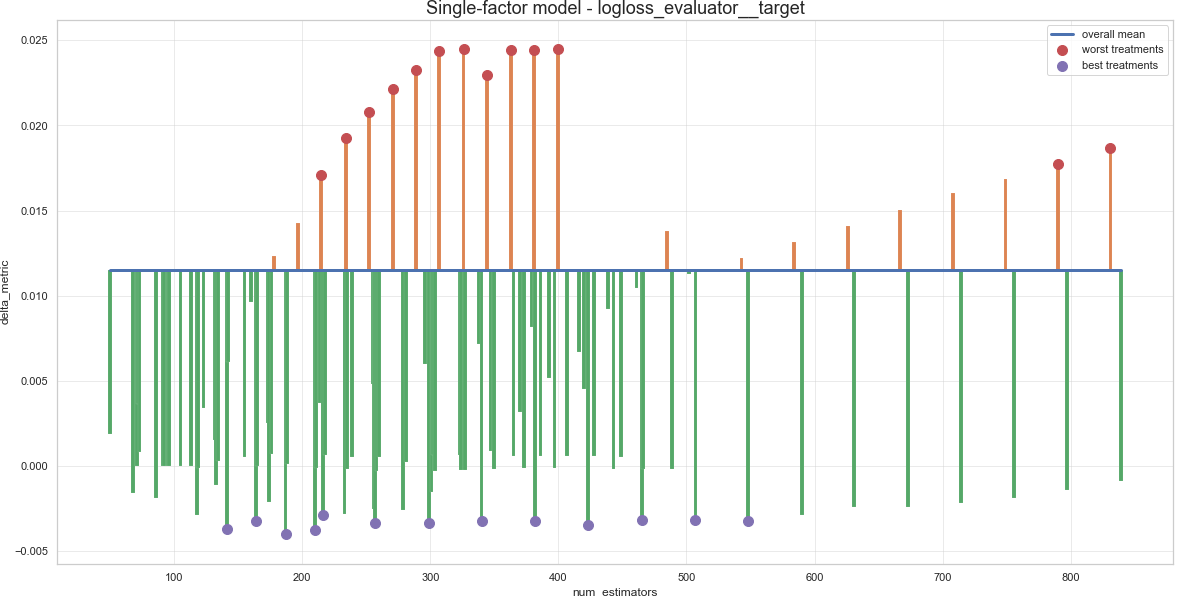
\includegraphics[width=.75\textwidth]{appendix_figures/sfm_logloss_cluster1_num_estimators.png}
    \caption{SFM plot for $\mathcal{S}(C_1, \eta^{(1)}_{NE}, Logloss)$}
\end{figure}


\begin{figure}[!ht]
    \centering
    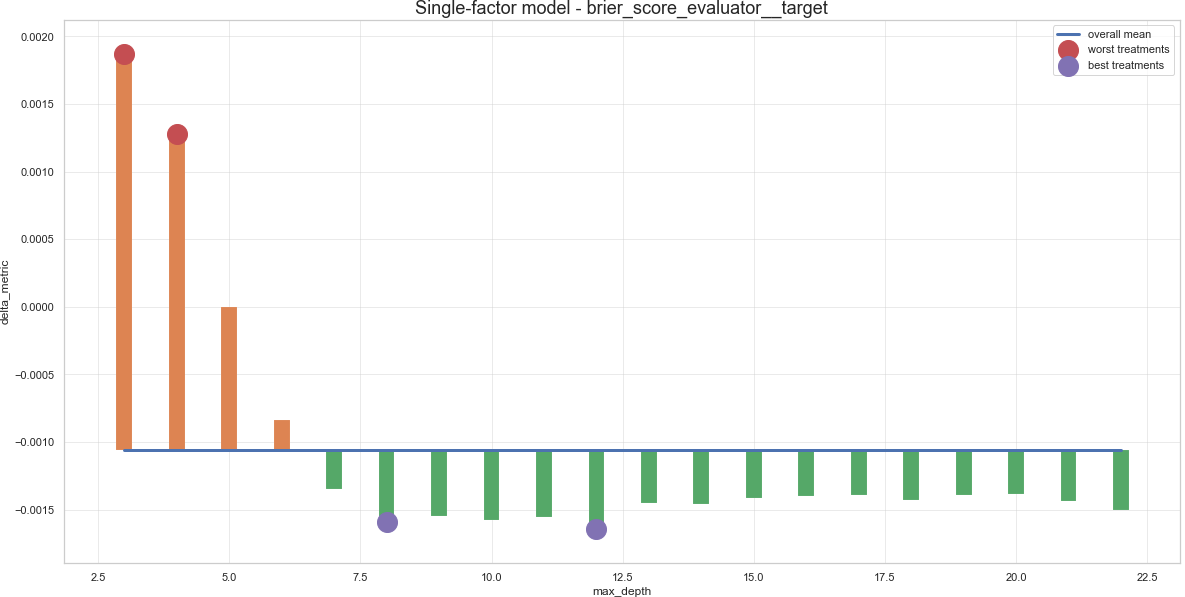
\includegraphics[width=.75\textwidth]{appendix_figures/sfm_brier_cluster1_max_depth.png}
    \caption{SFM plot for $\mathcal{S}(C_1, \eta^{(1)}_{MD}, Brier)$}
\end{figure}


% \begin{figure}[!ht]
%     \centering
%     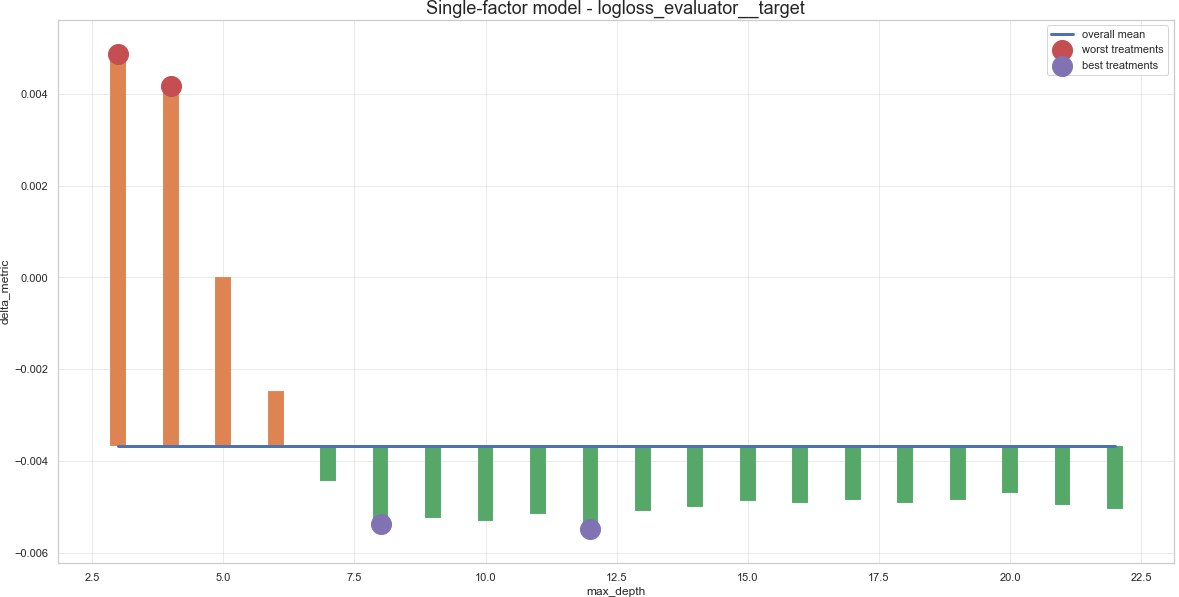
\includegraphics[width=.75\textwidth]{appendix_figures/sfm_logloss_cluster1_max_depth.png}
%     \caption{SFM plot for $\mathcal{S}(C_1, \eta^{(1)}_{MD}, Logloss)$}
% \end{figure}


% \begin{figure}[!ht]
%     \centering
%     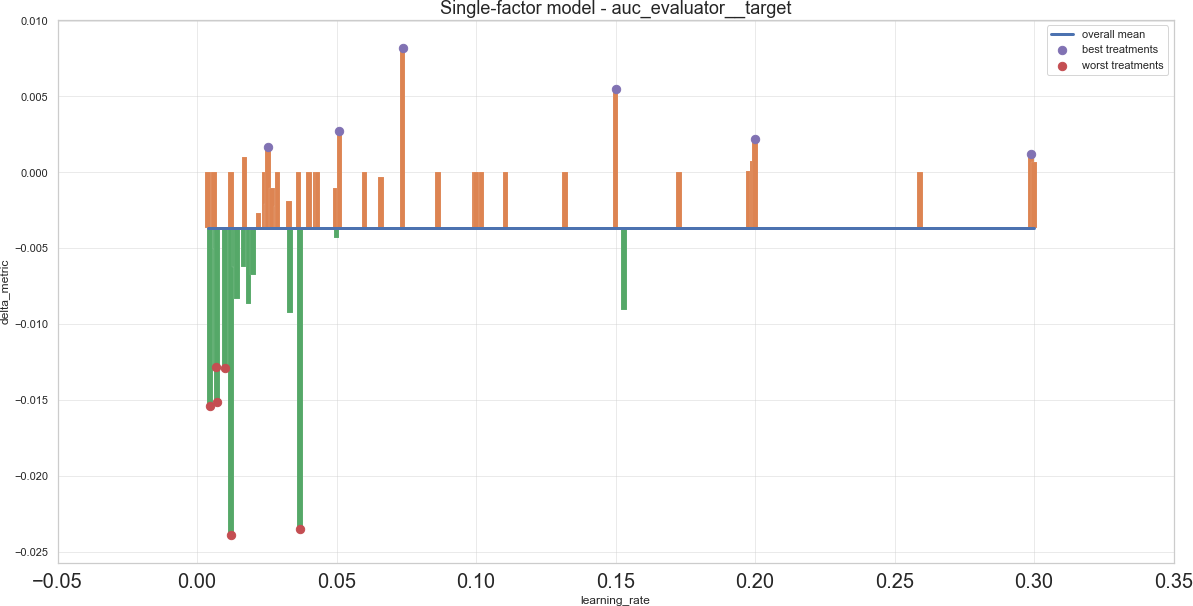
\includegraphics[width=.75\textwidth]{appendix_figures/sfm_auc_cluster1_learning_rate.png}
%     \caption{SFM plot for $\mathcal{S}(C_1, \eta^{(1)}_{LR}, AUC)$}
% \end{figure}


% \begin{figure}[!ht]
%     \centering
%     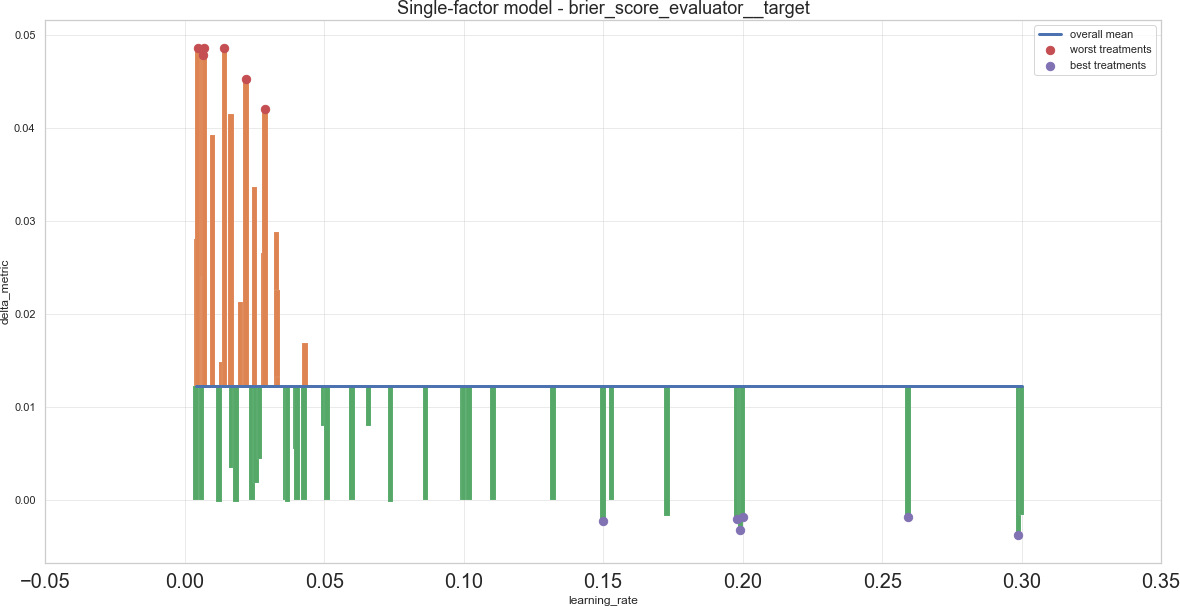
\includegraphics[width=.75\textwidth]{appendix_figures/sfm_brier_cluster1_learning_rate.png}
%     \caption{SFM plot for $\mathcal{S}(C_1, \eta^{(1)}_{LR}, Brier)$}
% \end{figure}


% \begin{figure}[!ht]
%     \centering
%     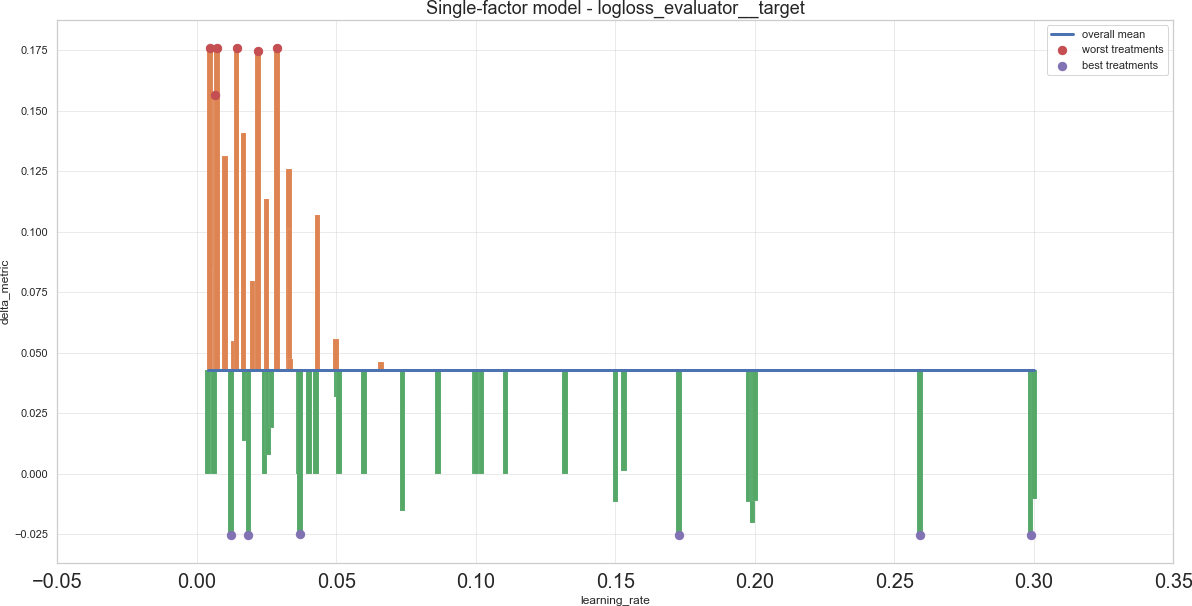
\includegraphics[width=.75\textwidth]{appendix_figures/sfm_logloss_cluster1_learning_rate.png}
%     \caption{SFM plot for $\mathcal{S}(C_1, \eta^{(1)}_{LR}, Logloss)$}
% \end{figure}


% \begin{figure}[!ht]
%     \centering
%     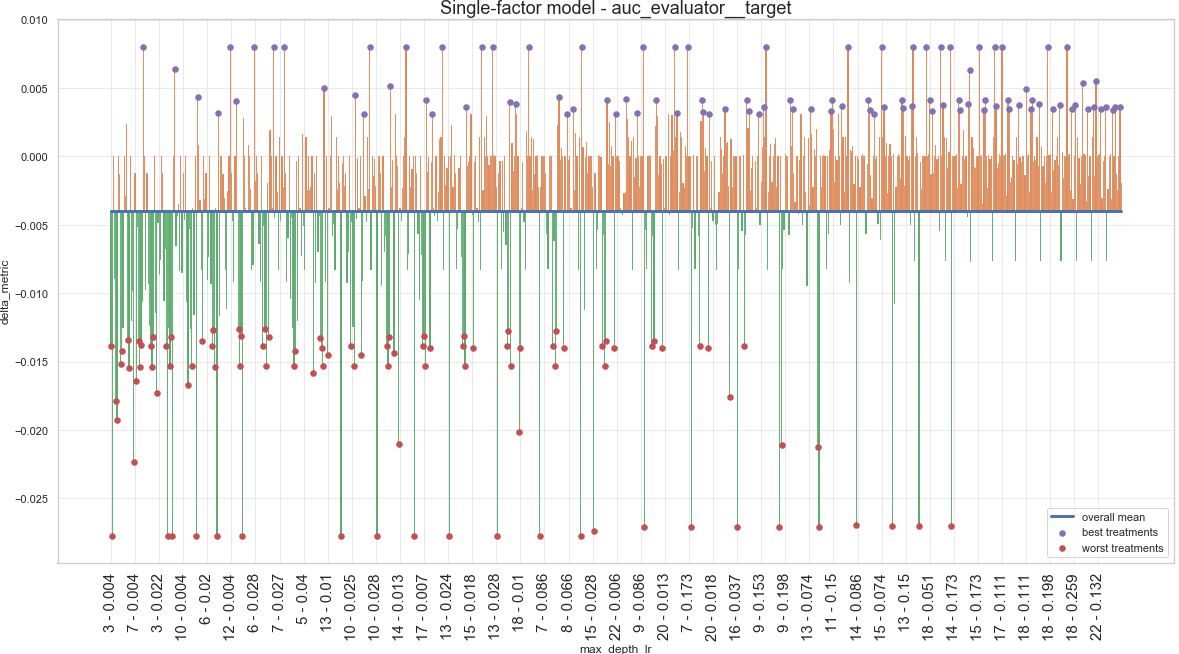
\includegraphics[width=.75\textwidth]{appendix_figures/sfm_auc_cluster1_max_depth_lr.png}
%     \caption{SFM plot for $\mathcal{S}(C_1, \eta^{(1)}_{MD, LR}, AUC)$}
% \end{figure}


% \begin{figure}[!ht]
%     \centering
%     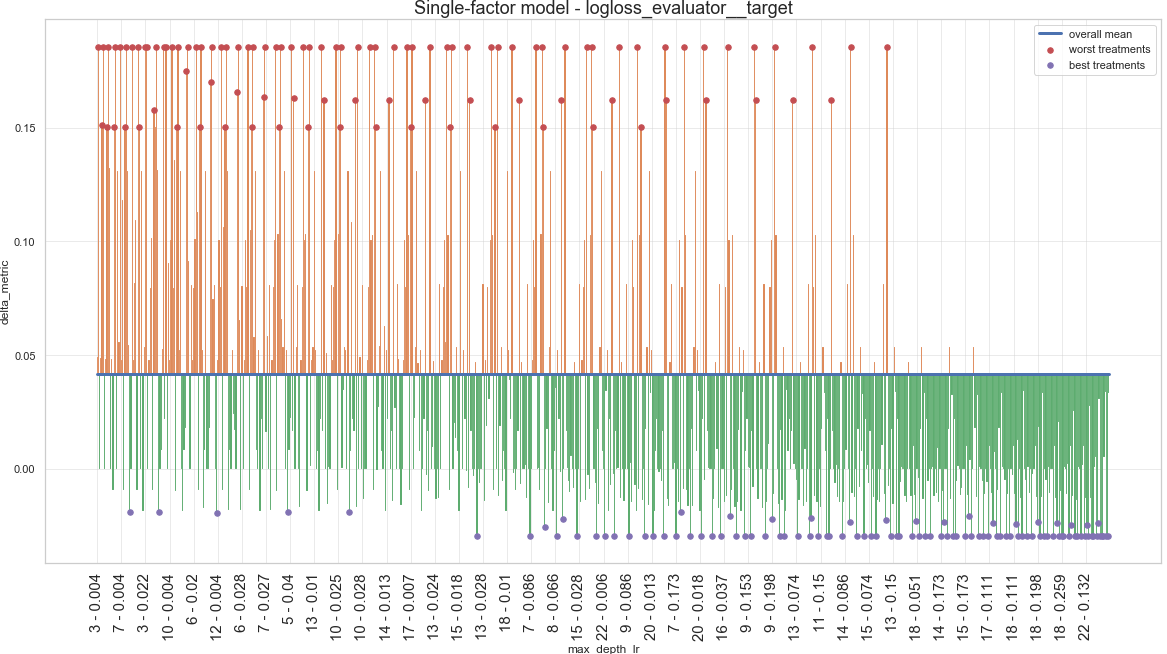
\includegraphics[width=.75\textwidth]{appendix_figures/sfm_logloss_cluster1_max_depth_lr.png}
%     \caption{SFM plot for $\mathcal{S}(C_1, \eta^{(1)}_{MD, LR}, Logloss)$}
% \end{figure}


% \begin{figure}[!ht]
%     \centering
%     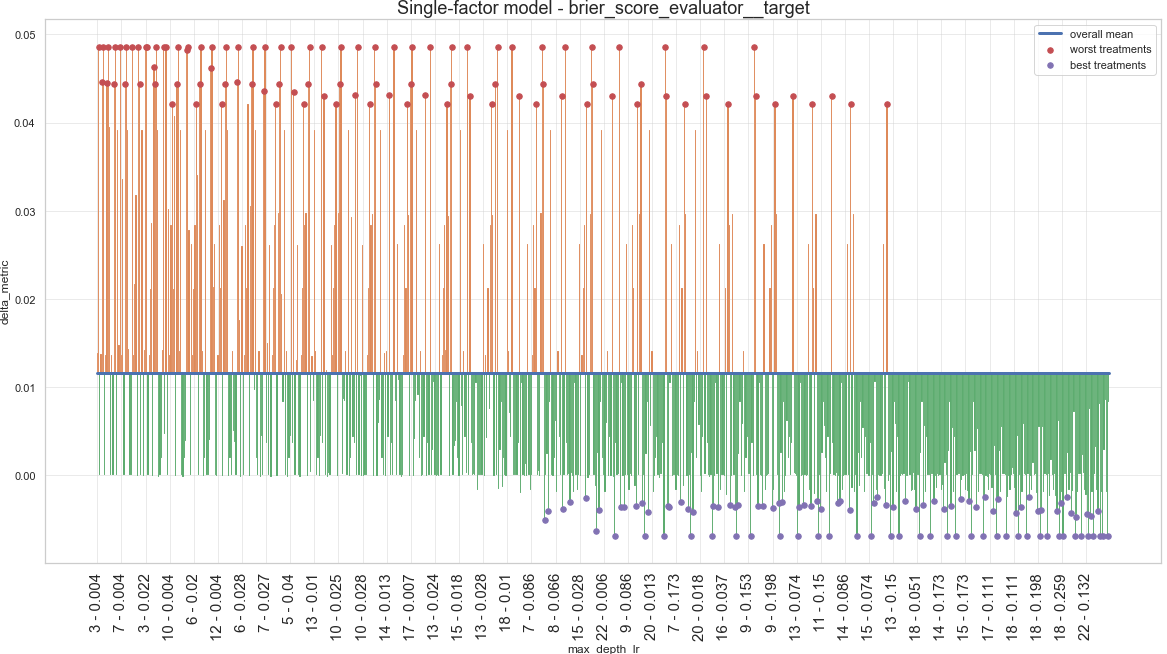
\includegraphics[width=.75\textwidth]{appendix_figures/sfm_brier_cluster1_max_depth_lr.png}
%     \caption{SFM plot for $\mathcal{S}(C_1, \eta^{(1)}_{MD, LR}, Brier)$}
% \end{figure}


% \begin{figure}[!ht]
%     \centering
%     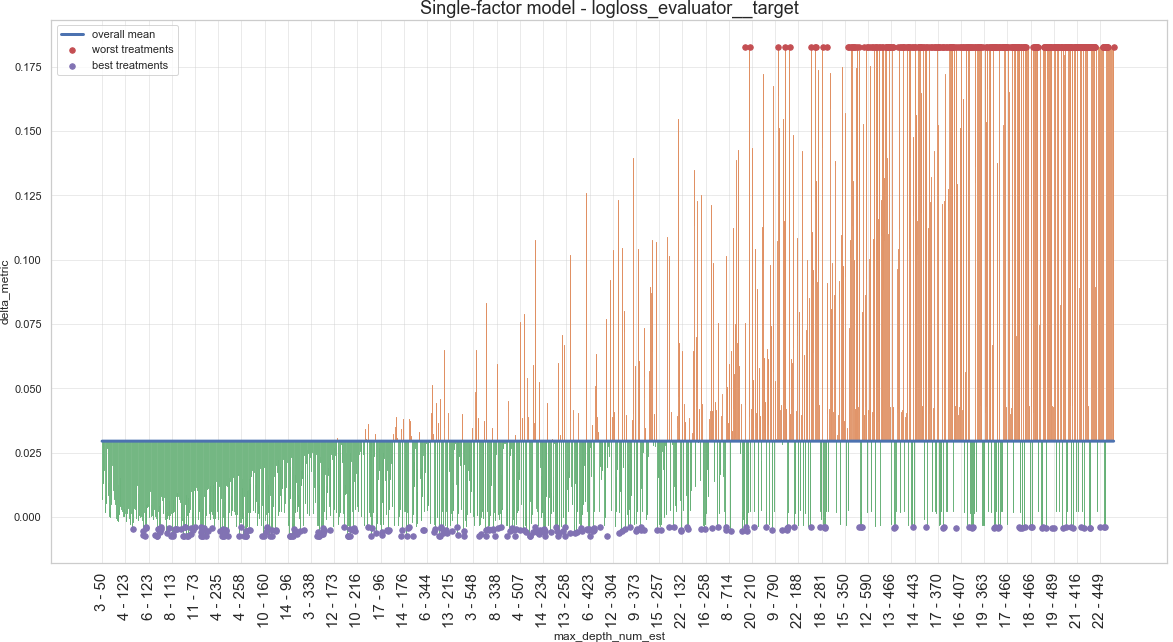
\includegraphics[width=.75\textwidth]{appendix_figures/sfm_logloss_cluster1_max_depth_num_est.png}
%     \caption{SFM plot for $\mathcal{S}(C_1, \eta^{(1)}_{MD, NE}, Logloss)$}
% \end{figure}


% \begin{figure}[!ht]
%     \centering
%     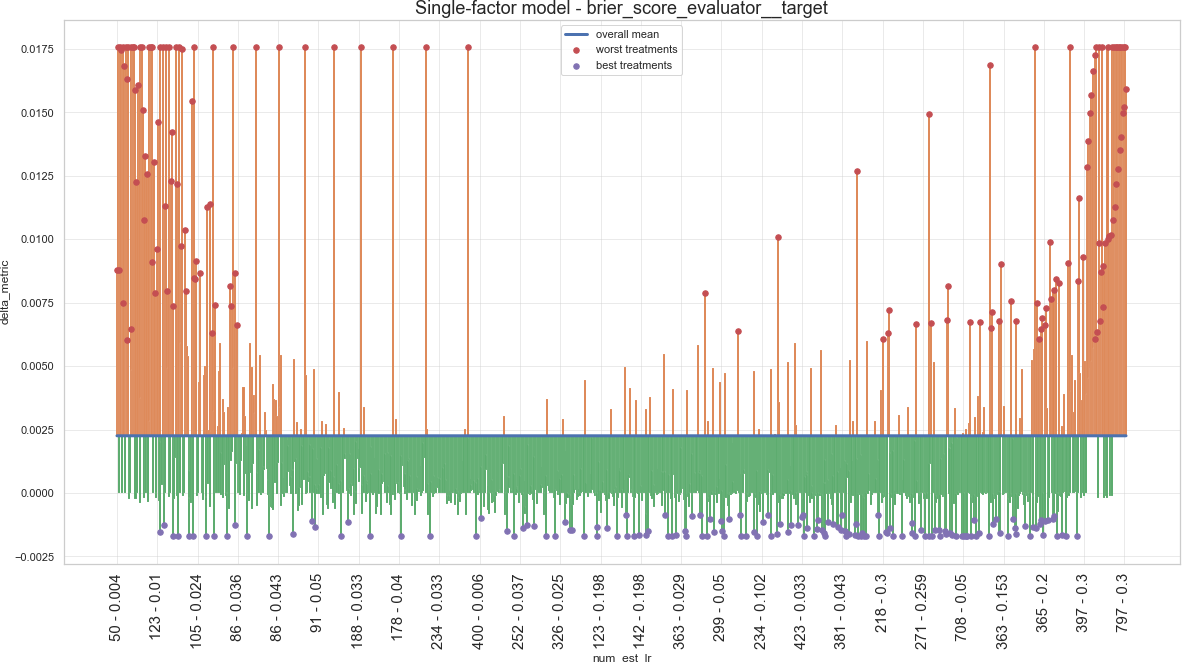
\includegraphics[width=.75\textwidth]{appendix_figures/sfm_brier_cluster1_num_est_lr.png}
%     \caption{SFM plot for $\mathcal{S}(C_1, \eta^{(1)}_{LR, NE}, Brier)$}
% \end{figure}


% \begin{figure}[!ht]
%     \centering
%     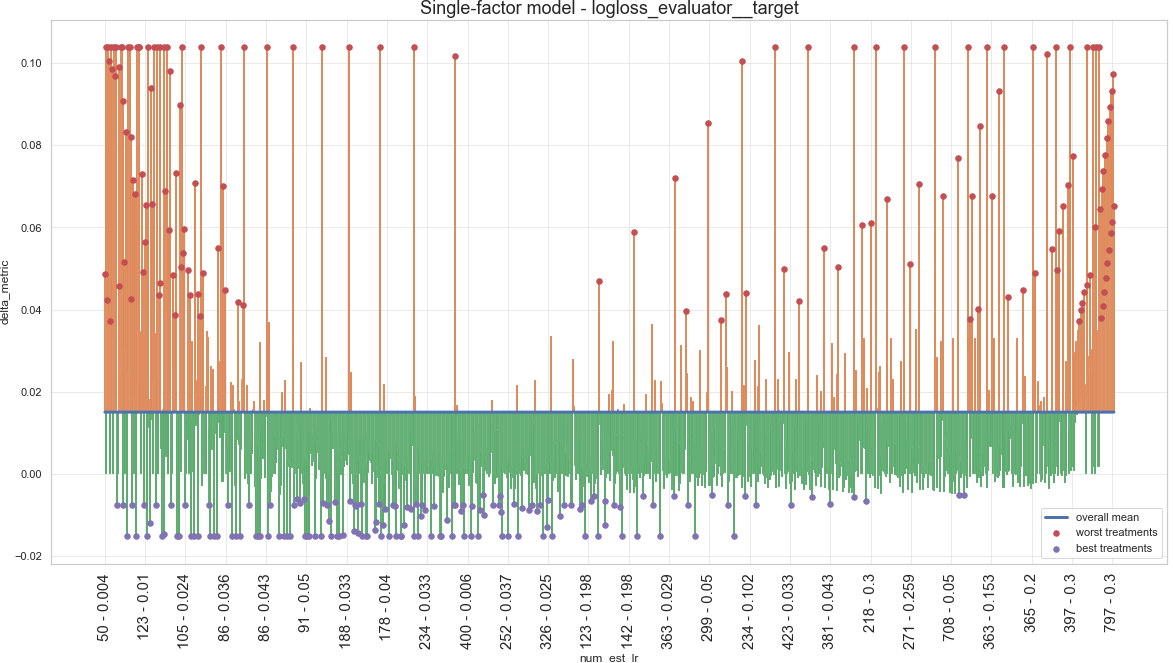
\includegraphics[width=.75\textwidth]{appendix_figures/sfm_logloss_cluster1_num_est_lr.png}
%     \caption{SFM plot for $\mathcal{S}(C_1, \eta^{(1)}_{LR, NE}, Logloss)$}
% \end{figure}


% \begin{figure}[!ht]
%     \centering
%     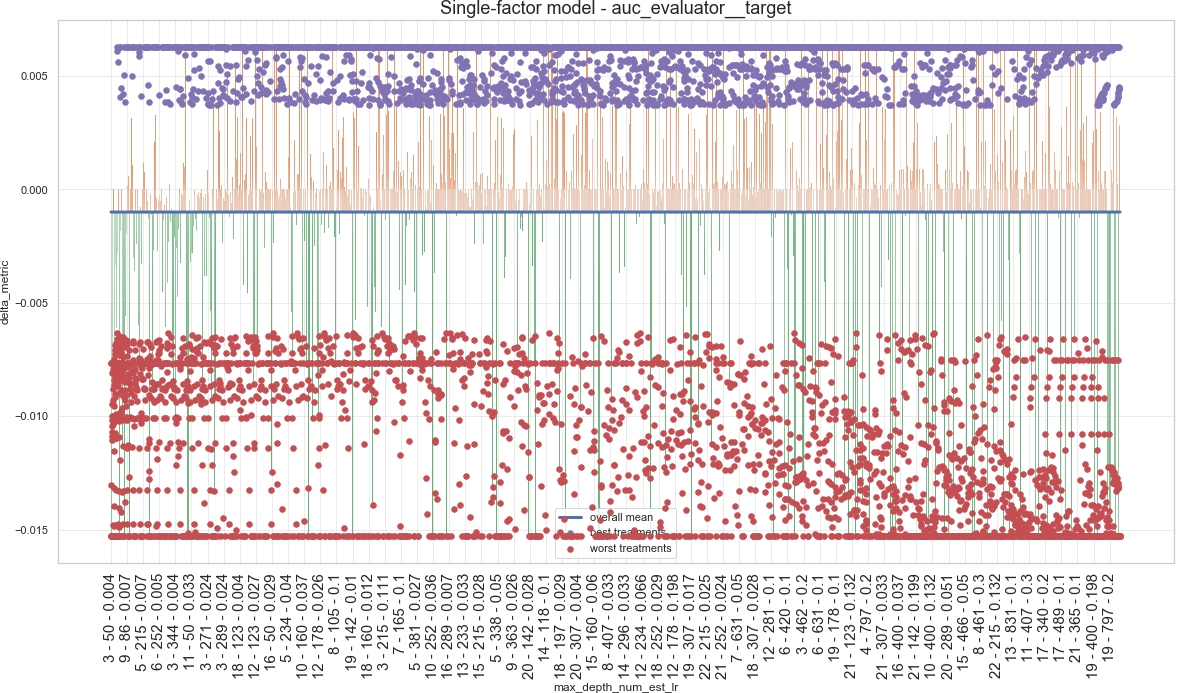
\includegraphics[width=.75\textwidth]{appendix_figures/sfm_auc_cluster1_max_depth_num_est_lr.png}
%     \caption{SFM plot for $\mathcal{S}(C_1, \eta^{(1)}_{NE, MD, LR}, AUC)$}
% \end{figure}


% \begin{figure}[!ht]
%     \centering
%     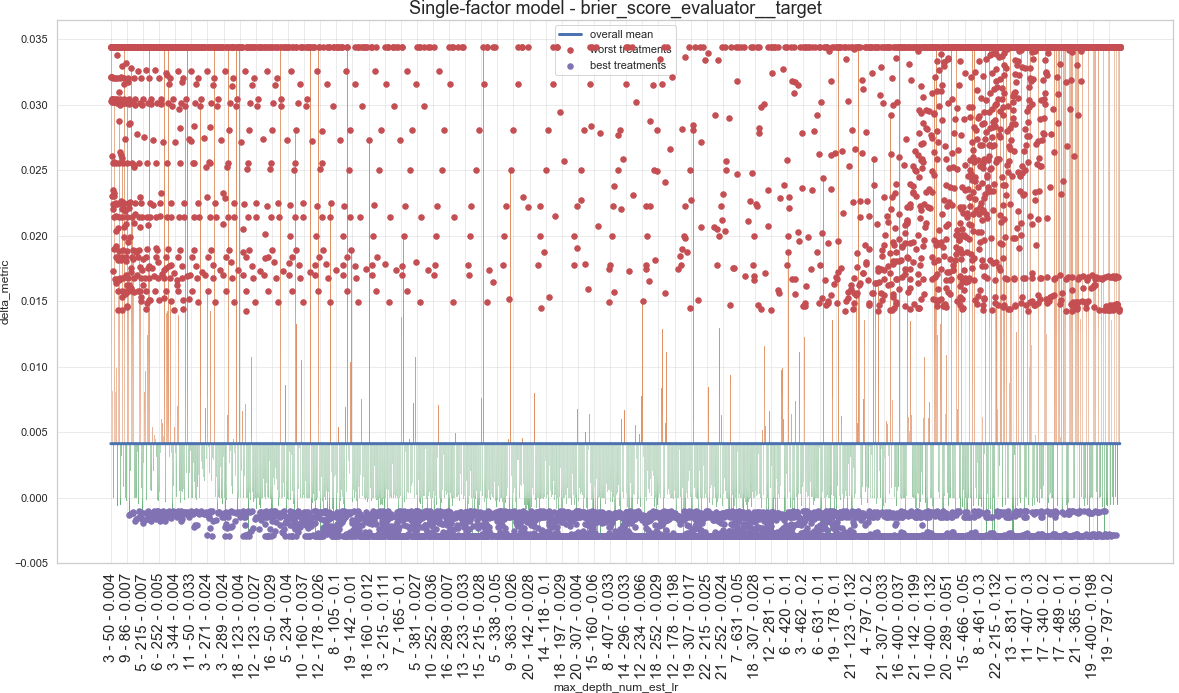
\includegraphics[width=.75\textwidth]{appendix_figures/sfm_brier_cluster1_max_depth_num_est_lr.png}
%     \caption{SFM plot for $\mathcal{S}(C_1, \eta^{(1)}_{NE, MD, LR}, Brier)$}
% \end{figure}


% \begin{figure}[!ht]
%     \centering
%     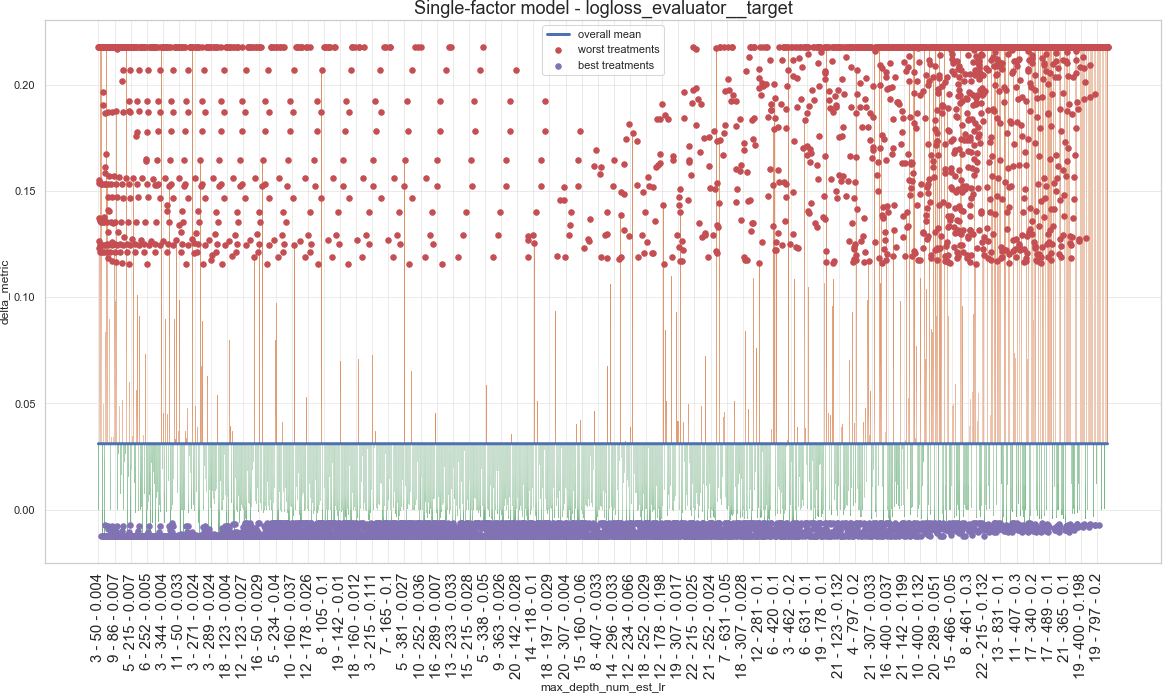
\includegraphics[width=.75\textwidth]{appendix_figures/sfm_logloss_cluster1_max_depth_num_est_lr.png}
%     \caption{SFM plot for $\mathcal{S}(C_1, \eta^{(1)}_{NE, MD, LR}, Logloss)$}
% \end{figure}


% \begin{figure}[!ht]
%     \centering
%     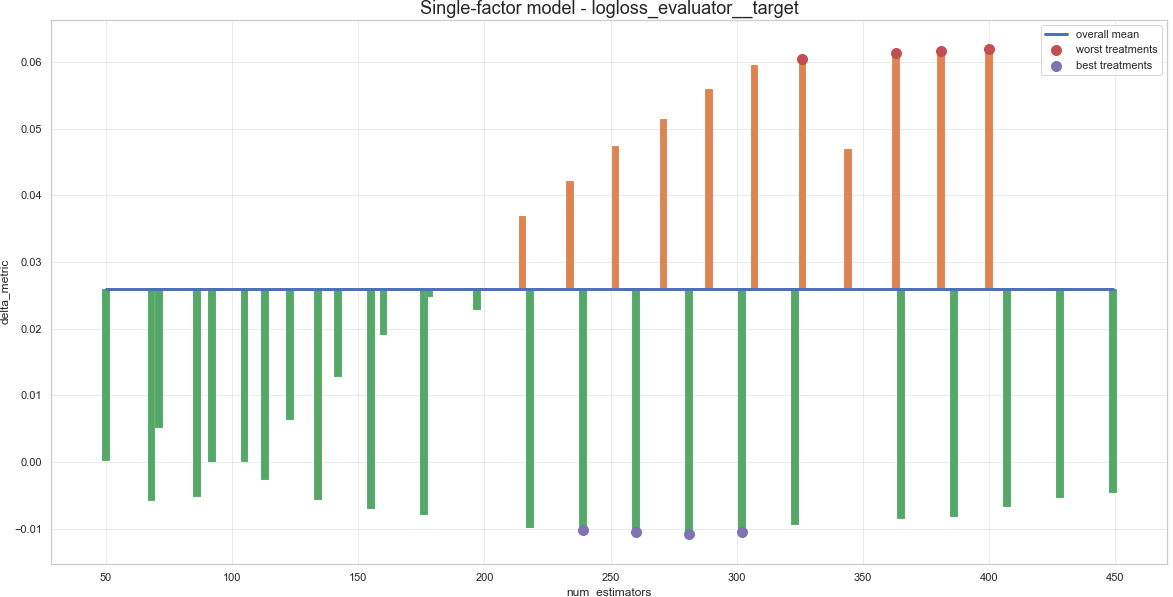
\includegraphics[width=.75\textwidth]{appendix_figures/sfm_logloss_cluster2_num_estimators.png}
%     \caption{SFM plot for $\mathcal{S}(C_2, \eta^{(2)}_{NE}, Logloss)$}
% \end{figure}


% \begin{figure}[!ht]
%     \centering
%     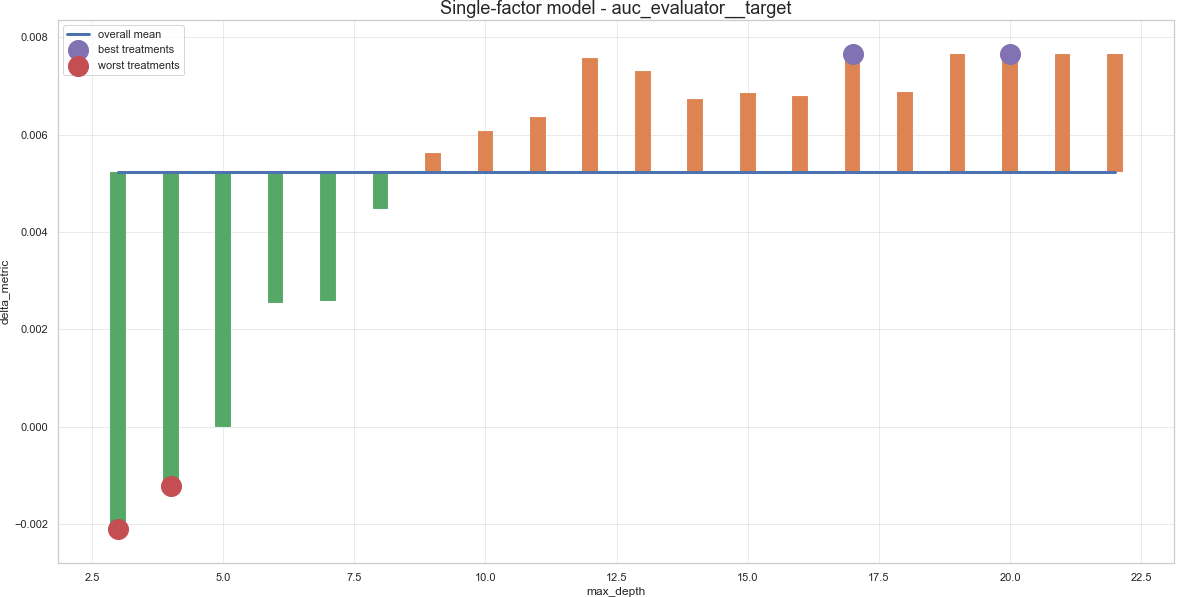
\includegraphics[width=.75\textwidth]{appendix_figures/sfm_auc_cluster2_max_depth.png}
%     \caption{SFM plot for $\mathcal{S}(C_2, \eta^{(2)}_{MD}, AUC)$}
% \end{figure}


% \begin{figure}[!ht]
%     \centering
%     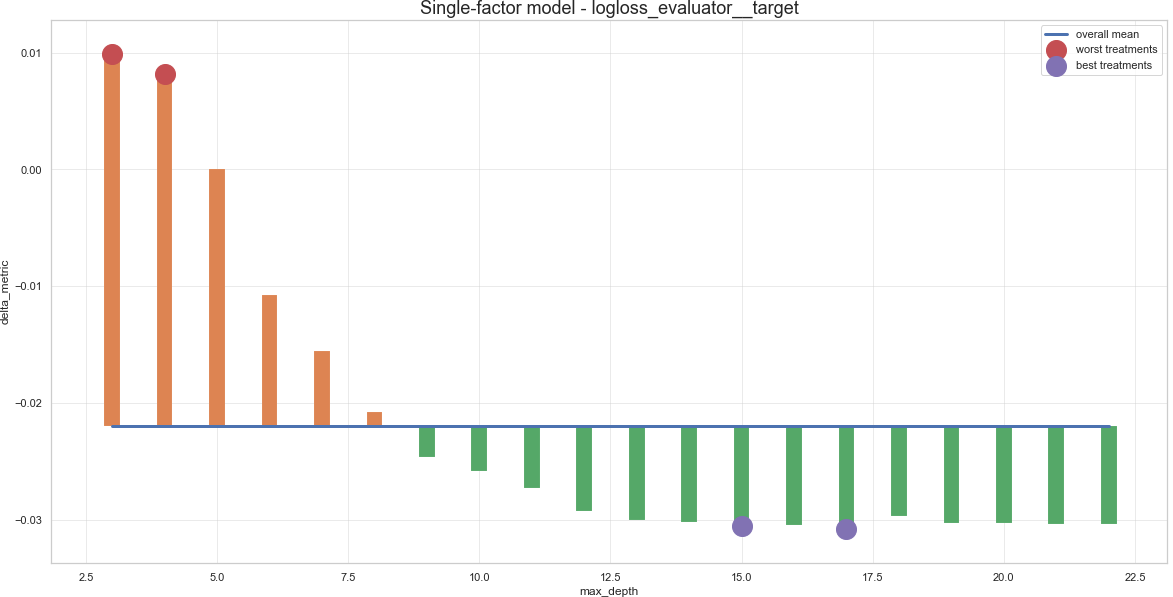
\includegraphics[width=.75\textwidth]{appendix_figures/sfm_logloss_cluster2_max_depth.png}
%     \caption{SFM plot for $\mathcal{S}(C_2, \eta^{(2)}_{MD}, Logloss)$}
% \end{figure}


% \begin{figure}[!ht]
%     \centering
%     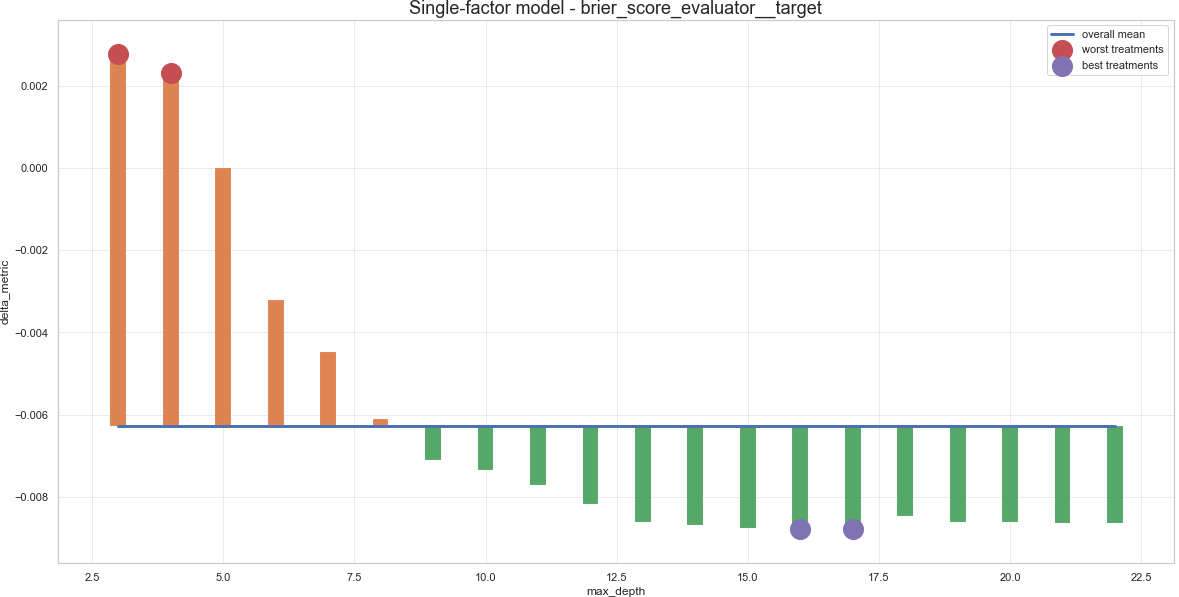
\includegraphics[width=.75\textwidth]{appendix_figures/sfm_brier_cluster2_max_depth.png}
%     \caption{SFM plot for $\mathcal{S}(C_2, \eta^{(2)}_{MD}, Brier)$}
% \end{figure}


% \begin{figure}[!ht]
%     \centering
%     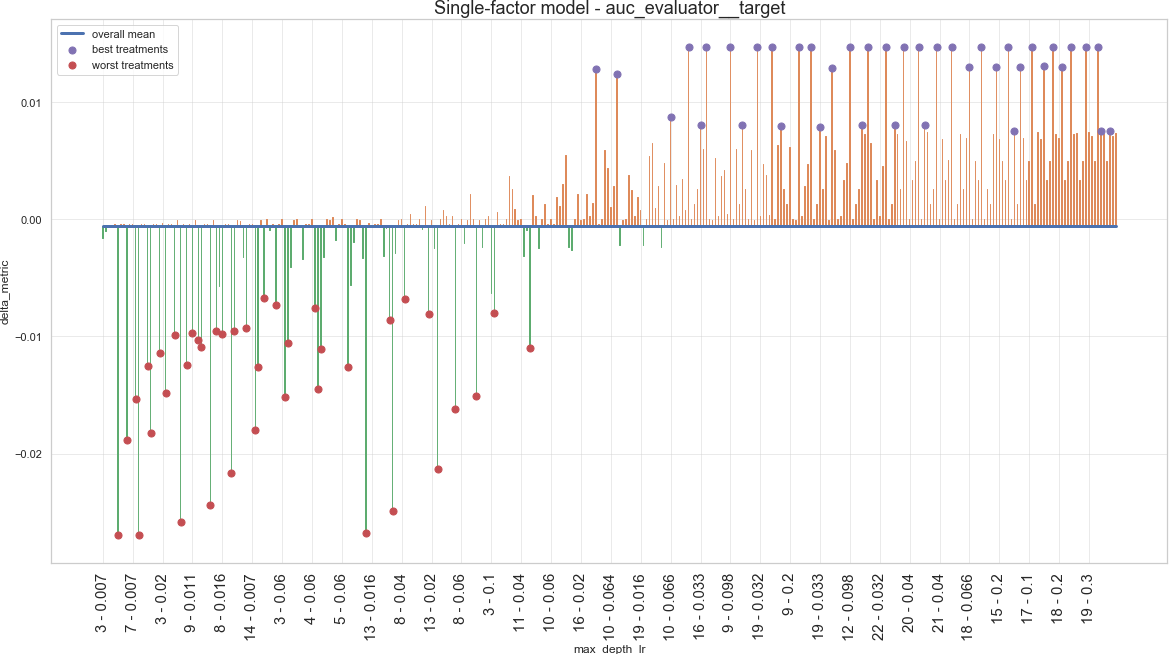
\includegraphics[width=.75\textwidth]{appendix_figures/sfm_auc_cluster2_max_depth_lr.png}
%     \caption{SFM plot for $\mathcal{S}(C_2, \eta^{(2)}_{MD, LR}, AUC)$}
% \end{figure}


% \begin{figure}[!ht]
%     \centering
%     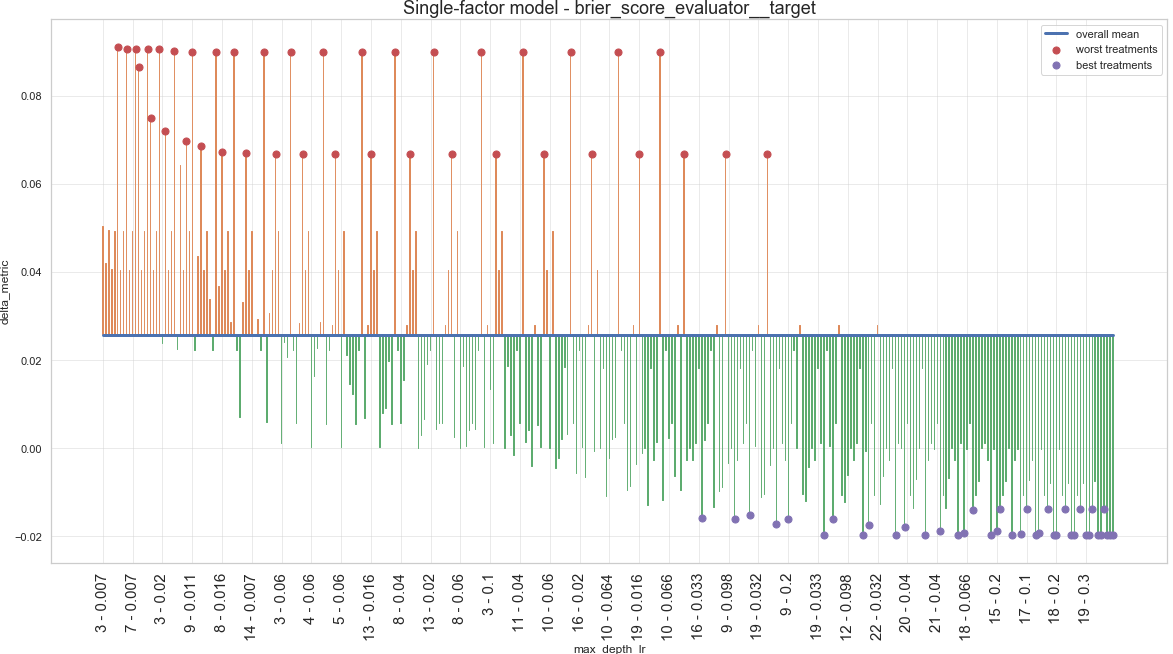
\includegraphics[width=.75\textwidth]{appendix_figures/sfm_brier_cluster2_max_depth_lr.png}
%     \caption{SFM plot for $\mathcal{S}(C_2, \eta^{(2)}_{MD, LR}, Brier)$}
% \end{figure}


% \begin{figure}[!ht]
%     \centering
%     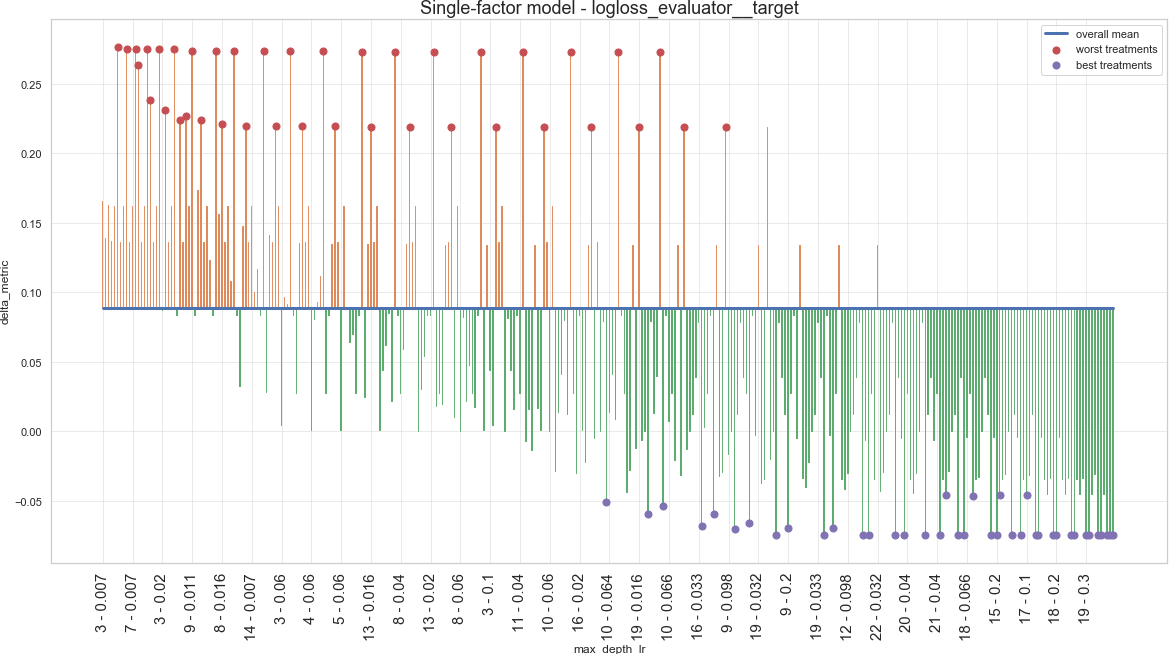
\includegraphics[width=.75\textwidth]{appendix_figures/sfm_logloss_cluster2_max_depth_lr.png}
%     \caption{SFM plot for $\mathcal{S}(C_2, \eta^{(2)}_{MD, LR}, Logloss)$}
% \end{figure}


% \begin{figure}[!ht]
%     \centering
%     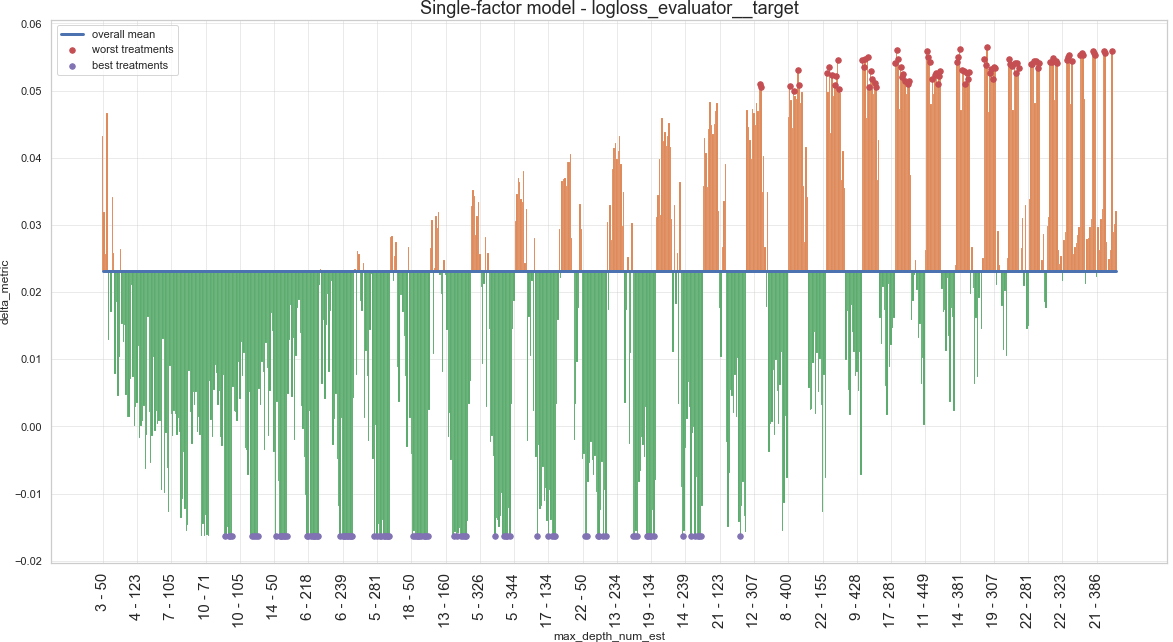
\includegraphics[width=.75\textwidth]{appendix_figures/sfm_logloss_cluster2_max_depth_num_est.png}
%     \caption{SFM plot for $\mathcal{S}(C_2, \eta^{(2)}_{MD, NE}, Logloss)$}
% \end{figure}


% \begin{figure}[!ht]
%     \centering
%     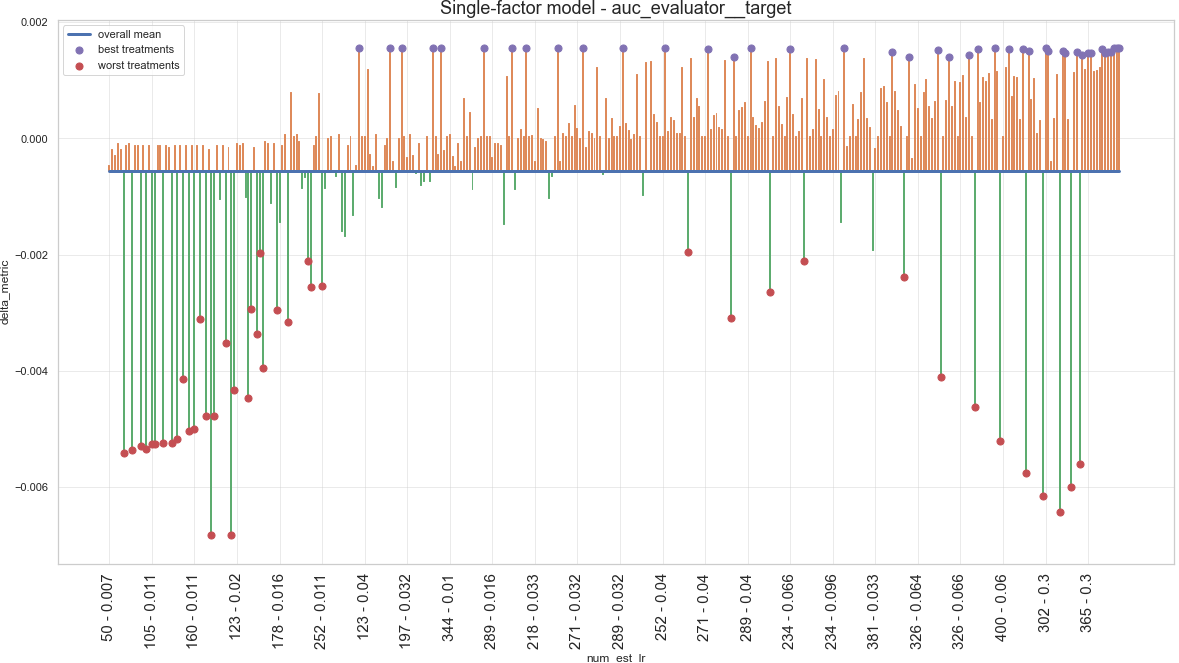
\includegraphics[width=.75\textwidth]{appendix_figures/sfm_auc_cluster2_num_est_lr.png}
%     \caption{SFM plot for $\mathcal{S}(C_2, \eta^{(2)}_{LR, NE}, AUC)$}
% \end{figure}


% \begin{figure}[!ht]
%     \centering
%     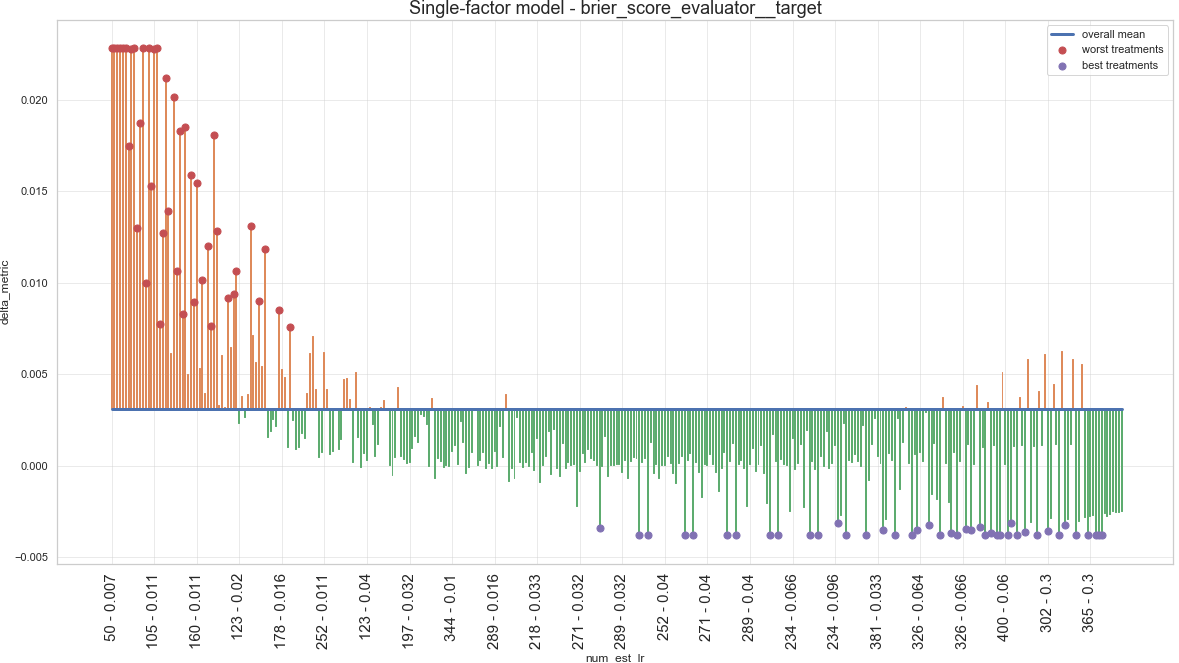
\includegraphics[width=.75\textwidth]{appendix_figures/sfm_brier_cluster2_num_est_lr.png}
%     \caption{SFM plot for $\mathcal{S}(C_2, \eta^{(2)}_{LR, NE}, Brier)$}
% \end{figure}


% \begin{figure}[!ht]
%     \centering
%     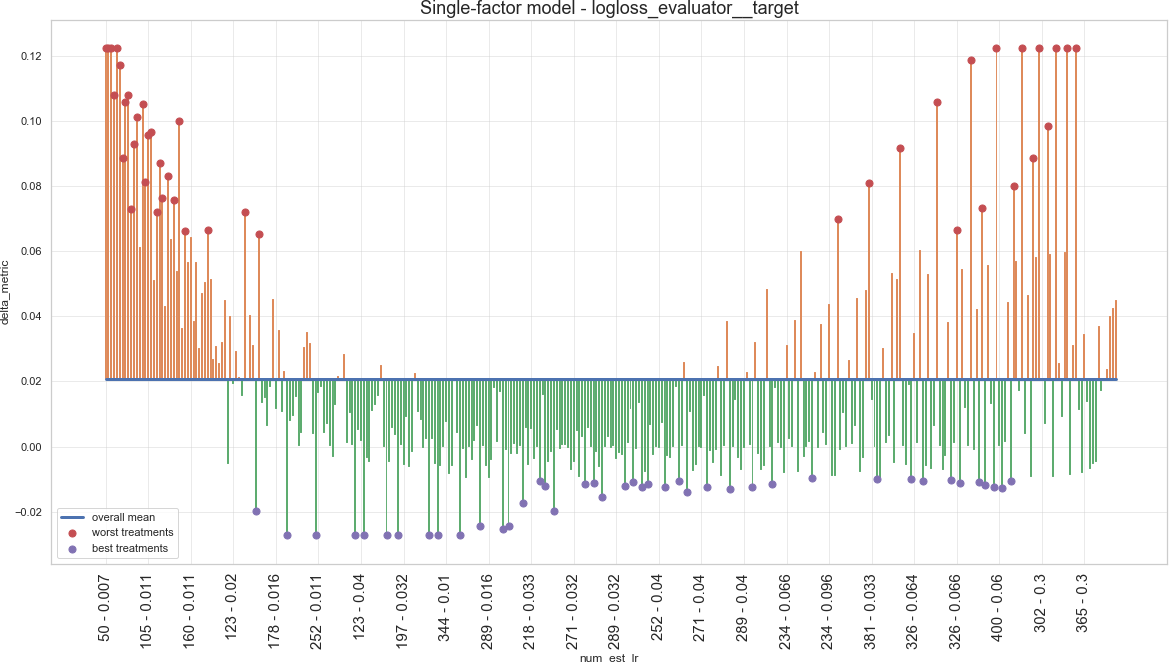
\includegraphics[width=.75\textwidth]{appendix_figures/sfm_logloss_cluster2_num_est_lr.png}
%     \caption{SFM plot for $\mathcal{S}(C_2, \eta^{(2)}_{LR, NE}, Logloss)$}
% \end{figure}


% \begin{figure}[!ht]
%     \centering
%     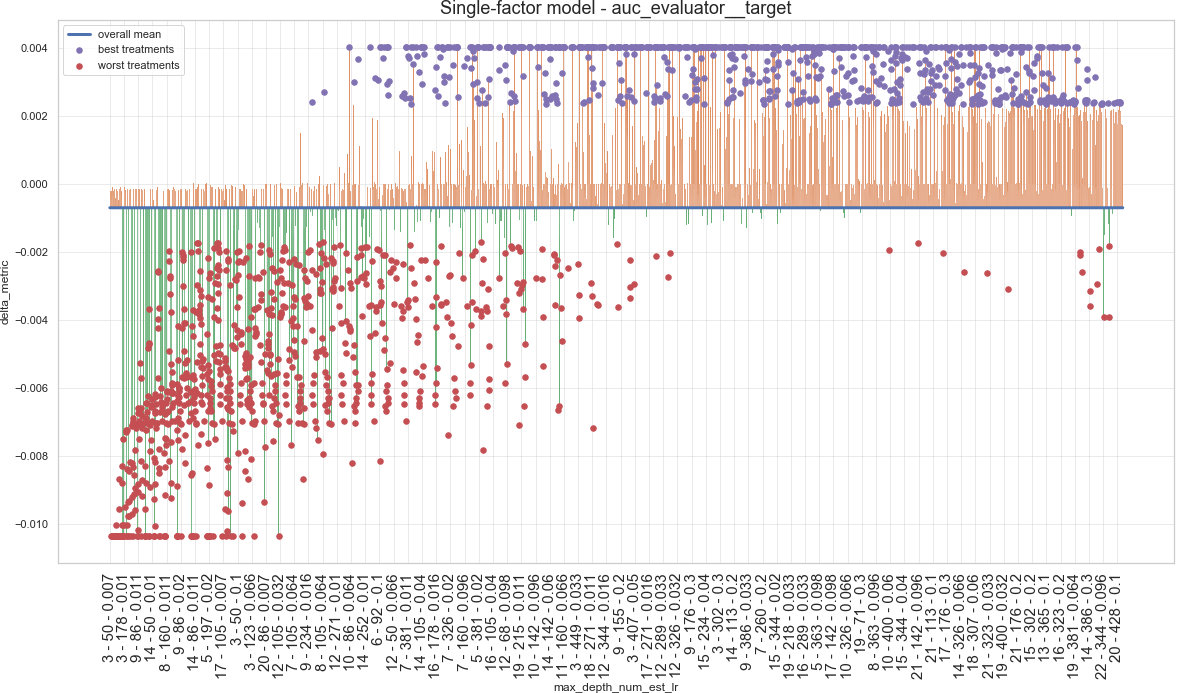
\includegraphics[width=.75\textwidth]{appendix_figures/sfm_auc_cluster2_max_depth_num_est_lr.png}
%     \caption{SFM plot for $\mathcal{S}(C_2, \eta^{(2)}_{NE, MD, LR}, AUC)$}
% \end{figure}


% \begin{figure}[!ht]
%     \centering
%     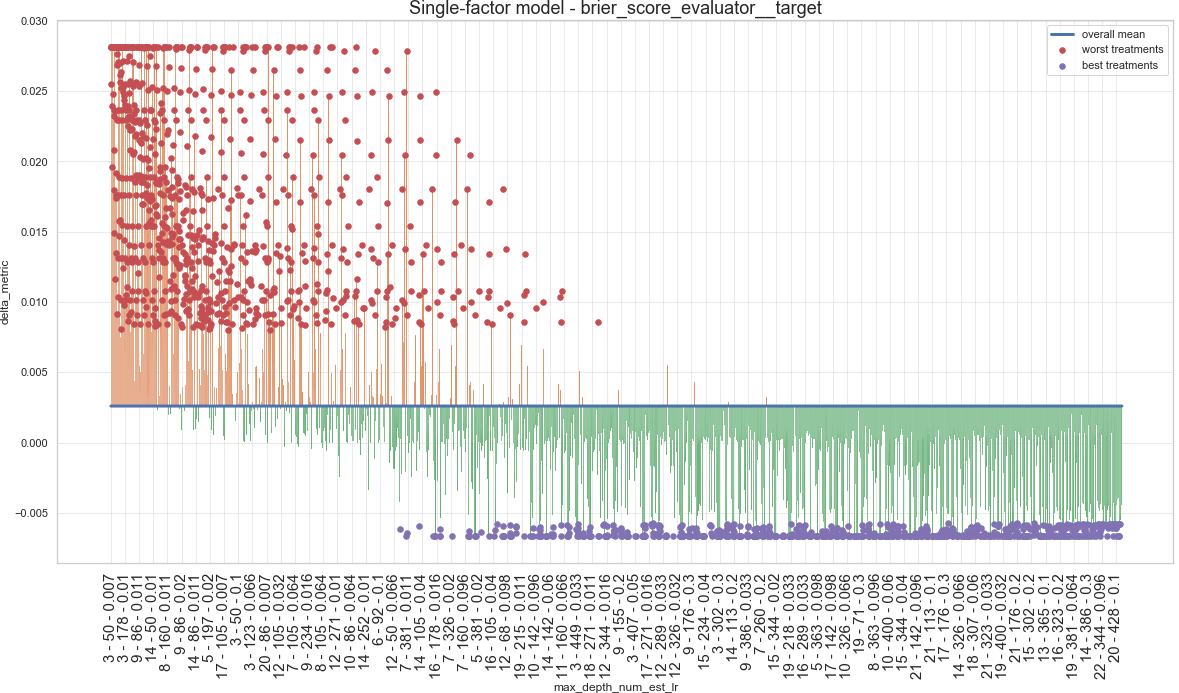
\includegraphics[width=.75\textwidth]{appendix_figures/sfm_brier_cluster2_max_depth_num_est_lr.png}
%     \caption{SFM plot for $\mathcal{S}(C_2, \eta^{(2)}_{NE, MD, LR}, Brier)$}
% \end{figure}


% \begin{figure}[!ht]
%     \centering
%     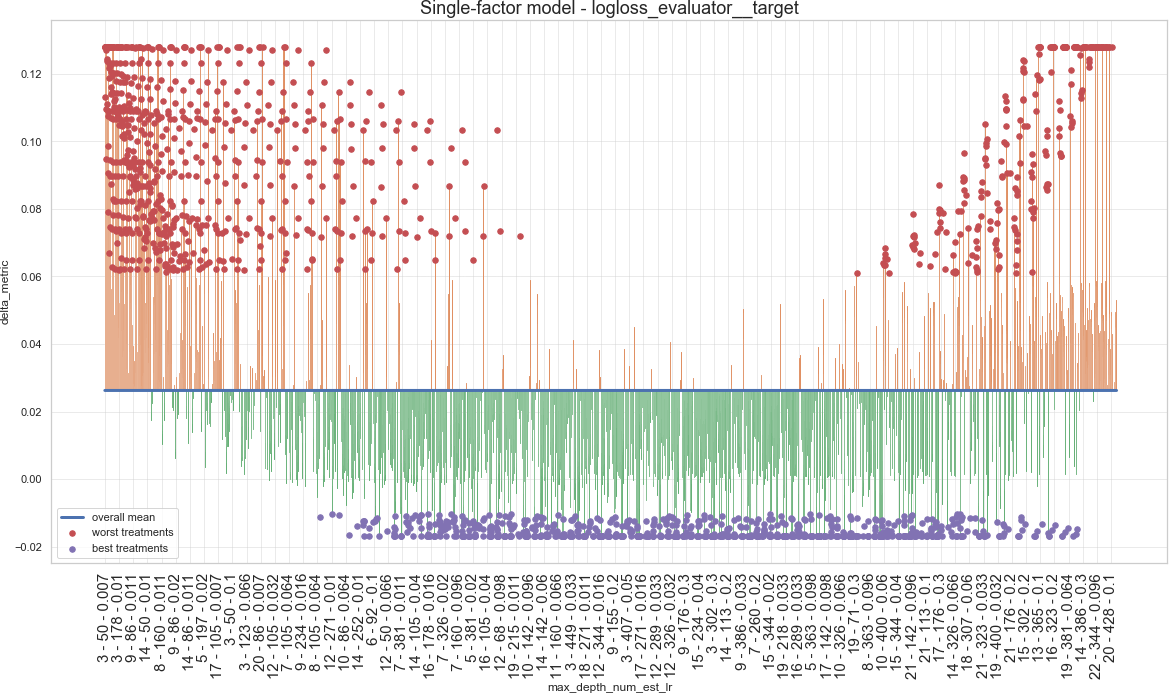
\includegraphics[width=.75\textwidth]{appendix_figures/sfm_logloss_cluster2_max_depth_num_est_lr.png}
%     \caption{SFM plot for $\mathcal{S}(C_2, \eta^{(2)}_{NE, MD, LR}, Logloss)$}
% \end{figure}


% \begin{figure}[!ht]
%     \centering
%     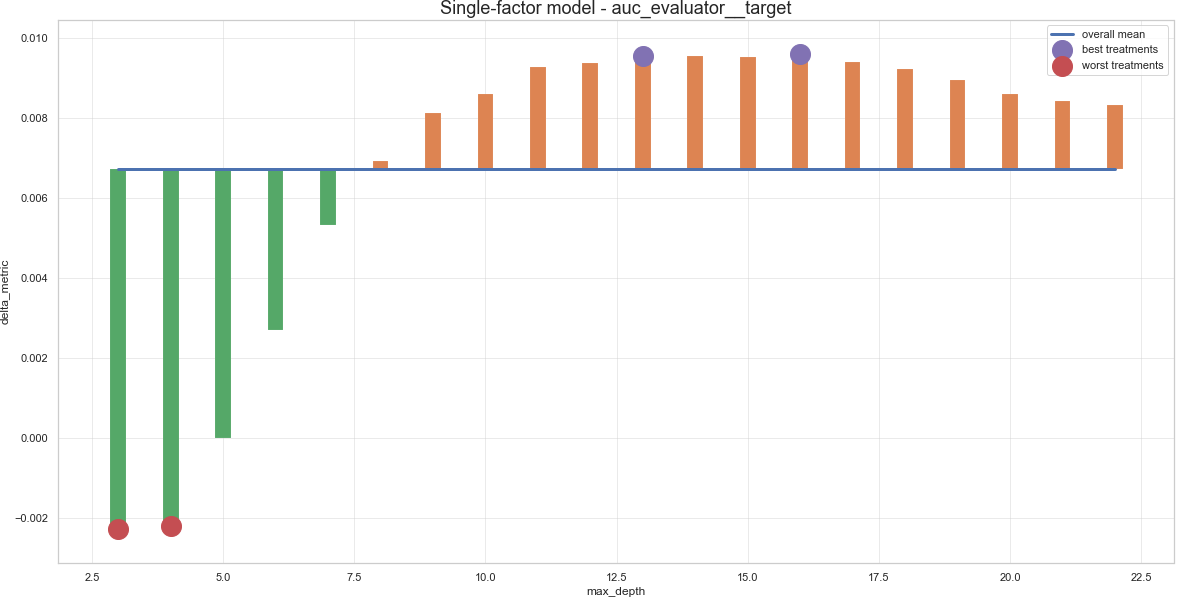
\includegraphics[width=.75\textwidth]{appendix_figures/sfm_auc_cluster3_max_depth.png}
%     \caption{SFM plot for $\mathcal{S}(C_3, \eta^{(3)}_{MD}, AUC)$}
% \end{figure}


% \begin{figure}[!ht]
%     \centering
%     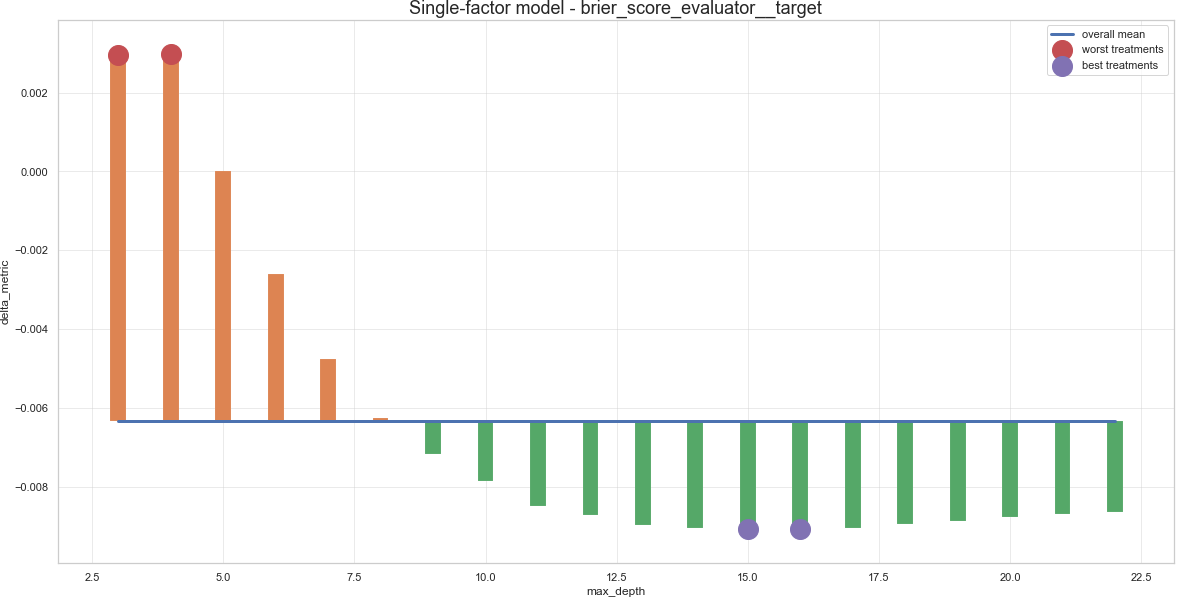
\includegraphics[width=.75\textwidth]{appendix_figures/sfm_brier_cluster3_max_depth.png}
%     \caption{SFM plot for $\mathcal{S}(C_3, \eta^{(3)}_{MD}, Brier)$}
% \end{figure}


% \begin{figure}[!ht]
%     \centering
%     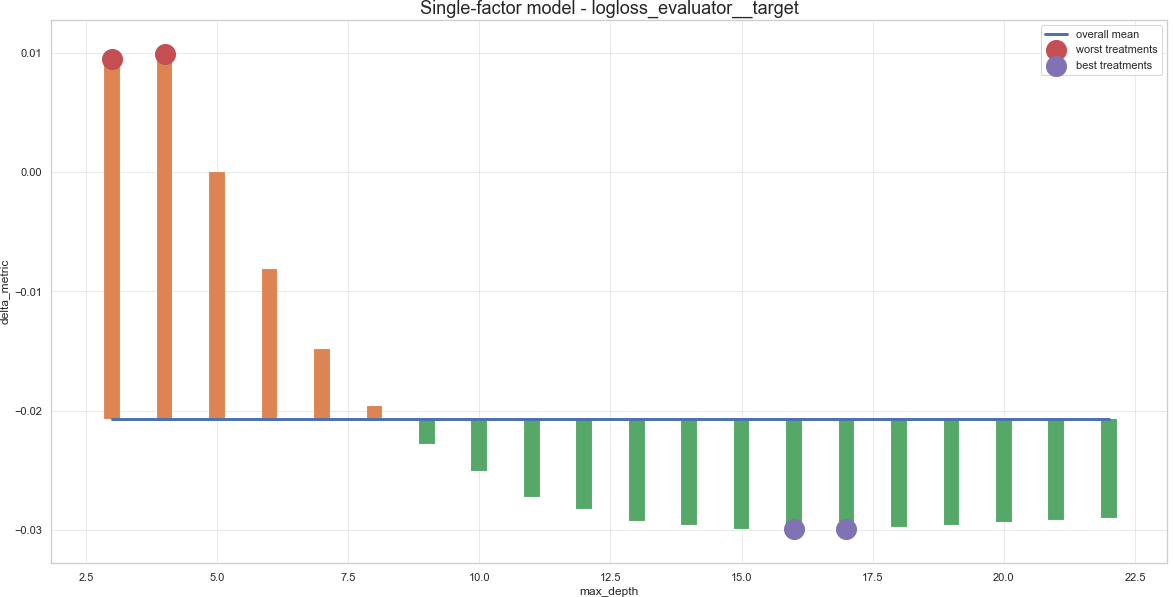
\includegraphics[width=.75\textwidth]{appendix_figures/sfm_logloss_cluster3_max_depth.png}
%     \caption{SFM plot for $\mathcal{S}(C_3, \eta^{(3)}_{MD}, Logloss)$}
% \end{figure}


% \begin{figure}[!ht]
%     \centering
%     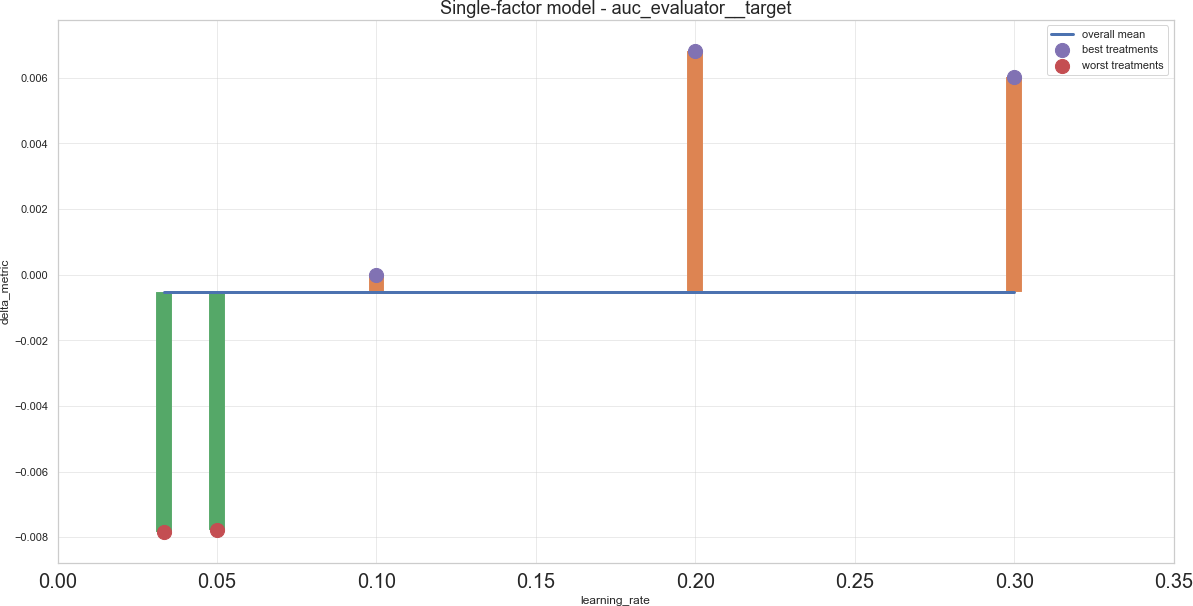
\includegraphics[width=.75\textwidth]{appendix_figures/sfm_auc_cluster3_learning_rate.png}
%     \caption{SFM plot for $\mathcal{S}(C_3, \eta^{(3)}_{LR}, AUC)$}
% \end{figure}


% \begin{figure}[!ht]
%     \centering
%     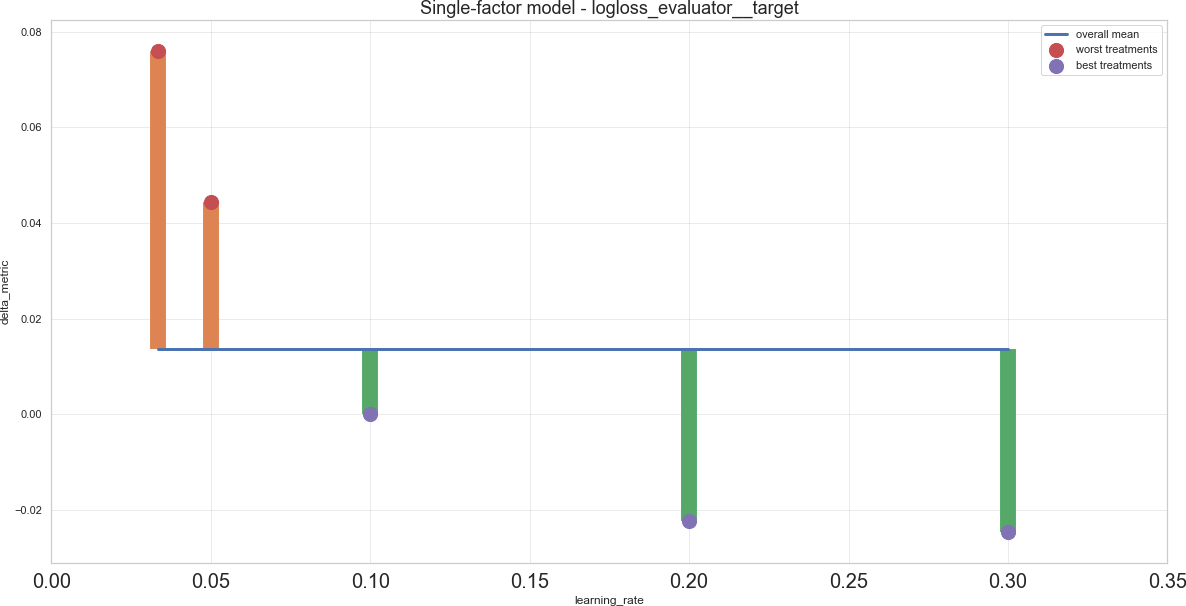
\includegraphics[width=.75\textwidth]{appendix_figures/sfm_logloss_cluster3_learning_rate.png}
%     \caption{SFM plot for $\mathcal{S}(C_3, \eta^{(3)}_{LR}, Logloss)$}
% \end{figure}


% \begin{figure}[!ht]
%     \centering
%     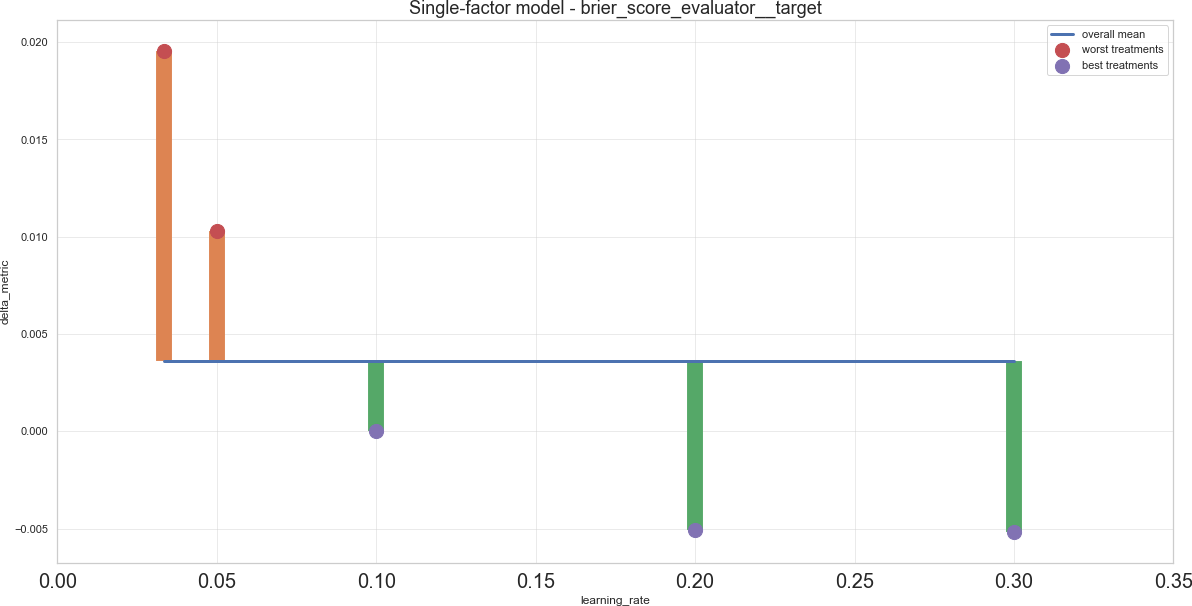
\includegraphics[width=.75\textwidth]{appendix_figures/sfm_brier_cluster3_learning_rate.png}
%     \caption{SFM plot for $\mathcal{S}(C_3, \eta^{(3)}_{LR}, Brier)$}
% \end{figure}


% \begin{figure}[!ht]
%     \centering
%     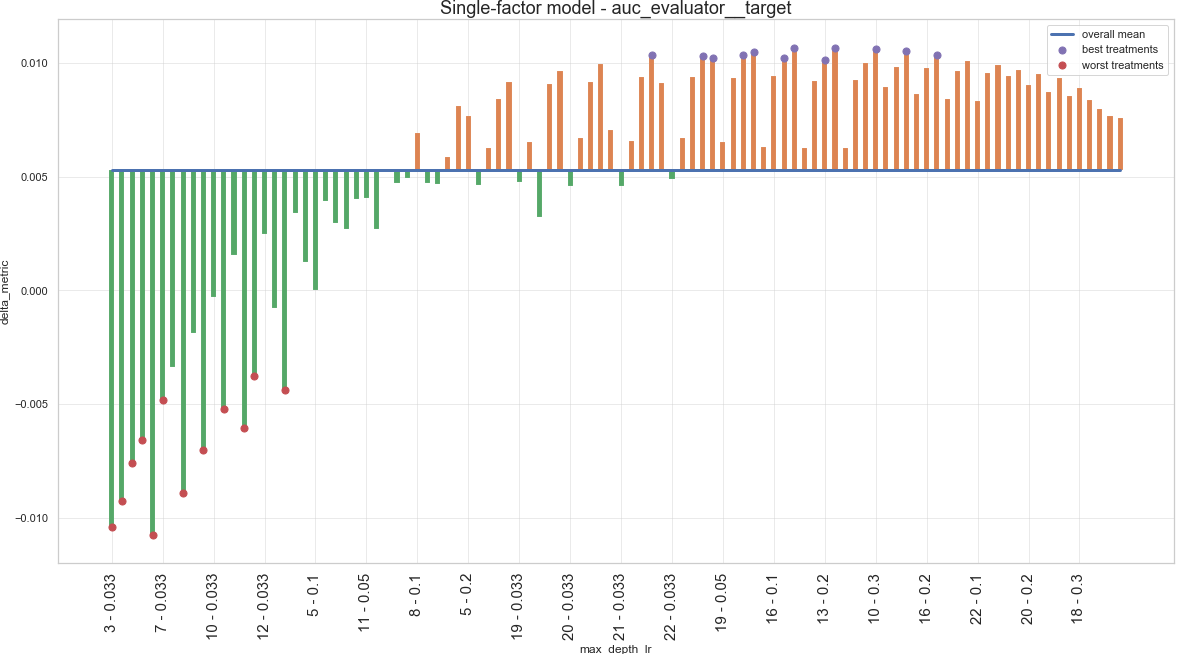
\includegraphics[width=.75\textwidth]{appendix_figures/sfm_auc_cluster3_max_depth_lr.png}
%     \caption{SFM plot for $\mathcal{S}(C_3, \eta^{(3)}_{MD, LR}, AUC)$}
% \end{figure}


% \begin{figure}[!ht]
%     \centering
%     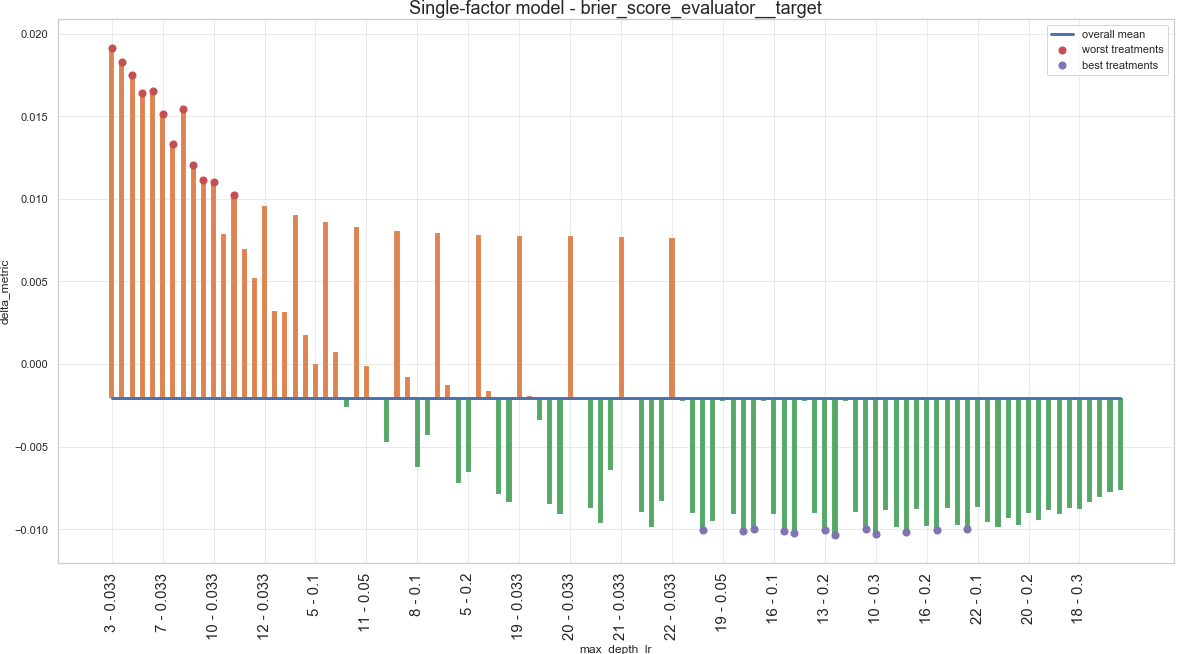
\includegraphics[width=.75\textwidth]{appendix_figures/sfm_brier_cluster3_max_depth_lr.png}
%     \caption{SFM plot for $\mathcal{S}(C_3, \eta^{(3)}_{MD, LR}, Brier)$}
% \end{figure}


% \begin{figure}[!ht]
%     \centering
%     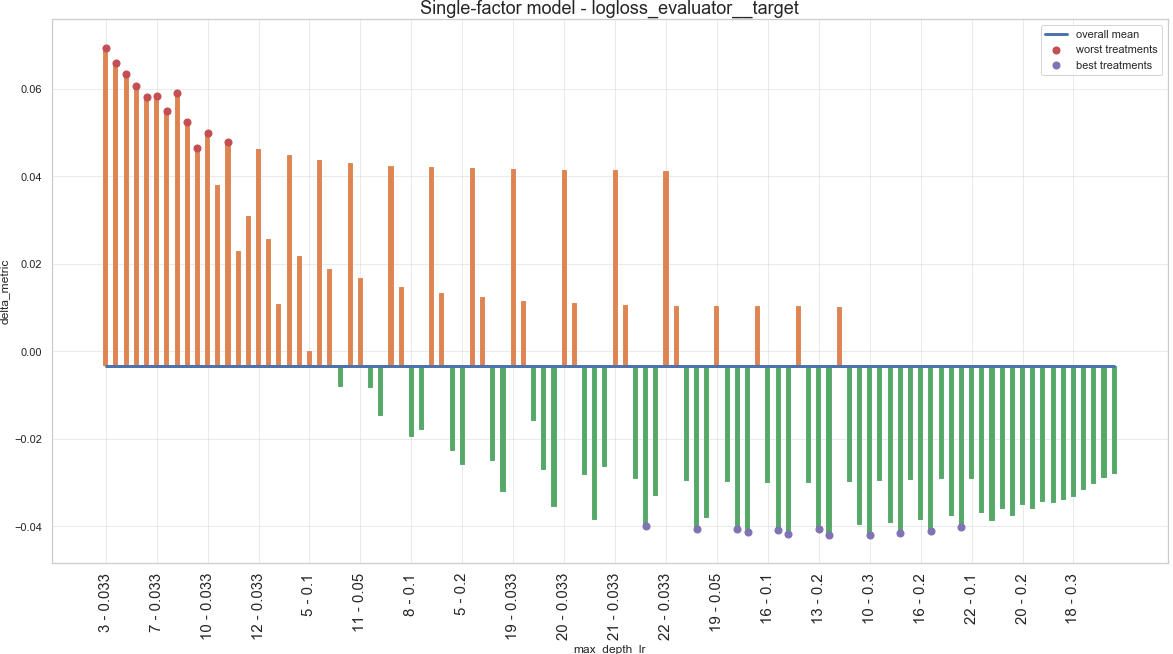
\includegraphics[width=.75\textwidth]{appendix_figures/sfm_logloss_cluster3_max_depth_lr.png}
%     \caption{SFM plot for $\mathcal{S}(C_3, \eta^{(3)}_{MD, LR}, Logloss)$}
% \end{figure}


% \begin{figure}[!ht]
%     \centering
%     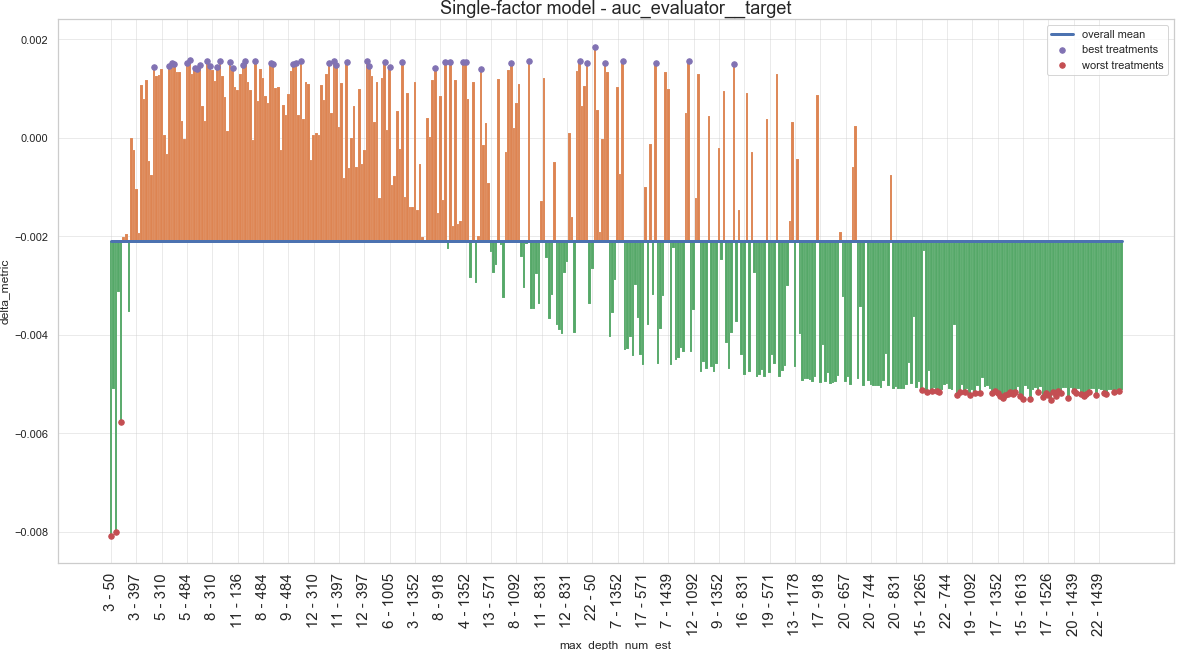
\includegraphics[width=.75\textwidth]{appendix_figures/sfm_auc_cluster3_max_depth_num_est.png}
%     \caption{SFM plot for $\mathcal{S}(C_3, \eta^{(3)}_{MD, NE}, AUC)$}
% \end{figure}


% \begin{figure}[!ht]
%     \centering
%     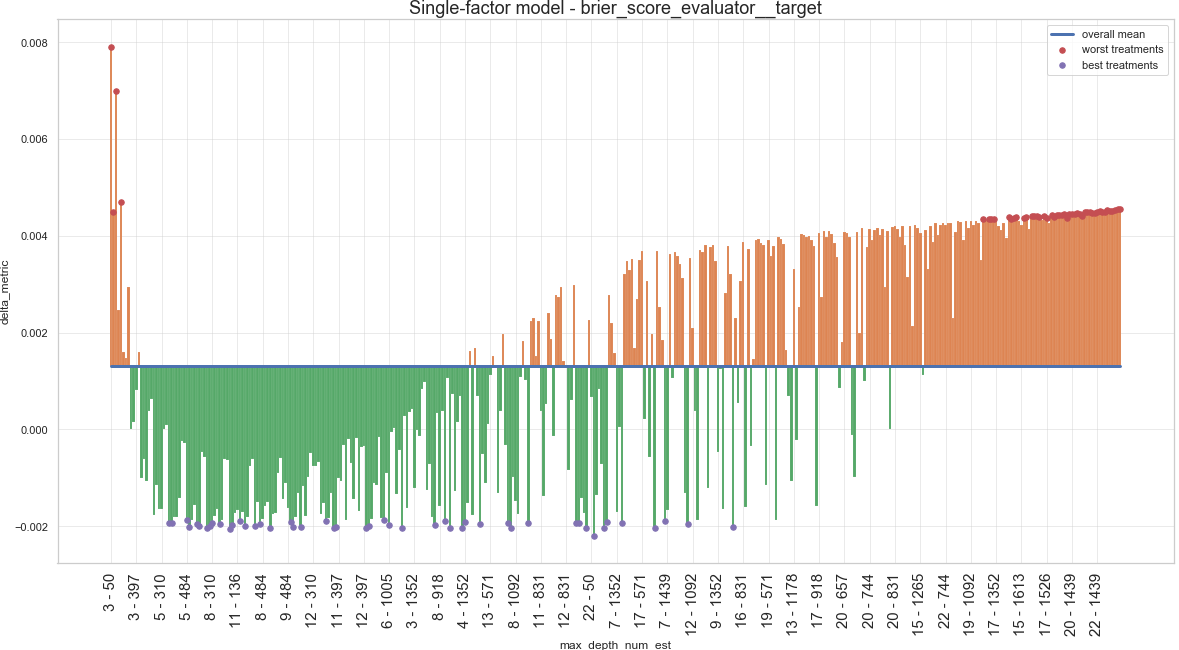
\includegraphics[width=.75\textwidth]{appendix_figures/sfm_brier_cluster3_max_depth_num_est.png}
%     \caption{SFM plot for $\mathcal{S}(C_3, \eta^{(3)}_{MD, NE}, Brier)$}
% \end{figure}


% \begin{figure}[!ht]
%     \centering
%     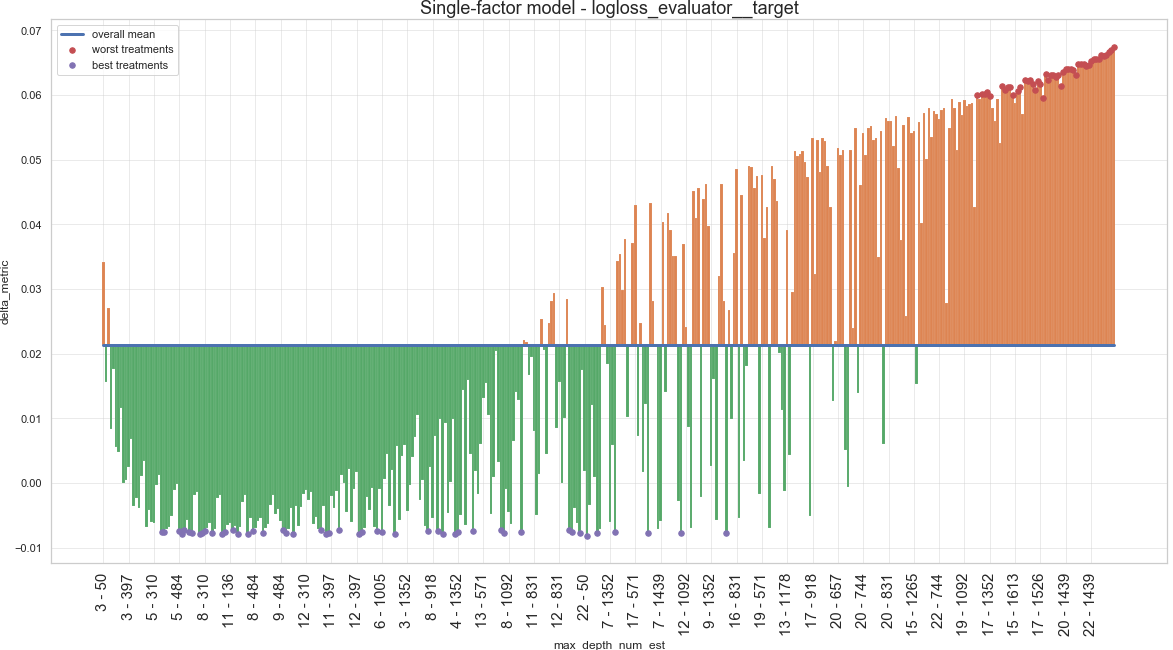
\includegraphics[width=.75\textwidth]{appendix_figures/sfm_logloss_cluster3_max_depth_num_est.png}
%     \caption{SFM plot for $\mathcal{S}(C_3, \eta^{(3)}_{MD, NE}, Logloss)$}
% \end{figure}


% \begin{figure}[!ht]
%     \centering
%     \includegraphics[width=.75\textwidth]{appendix_figures/sfm_auc_cluster3_num_est_lr.png}
%     \caption{SFM plot for $\mathcal{S}(C_3, \eta^{(3)}_{LR, NE}, AUC)$}
% \end{figure}


% \begin{figure}[!ht]
%     \centering
%     \includegraphics[width=.75\textwidth]{appendix_figures/sfm_brier_cluster3_num_est_lr.png}
%     \caption{SFM plot for $\mathcal{S}(C_3, \eta^{(3)}_{LR, NE}, Brier)$}
% \end{figure}


% \begin{figure}[!ht]
%     \centering
%     \includegraphics[width=.75\textwidth]{appendix_figures/sfm_logloss_cluster3_num_est_lr.png}
%     \caption{SFM plot for $\mathcal{S}(C_3, \eta^{(3)}_{LR, NE}, Logloss)$}
% \end{figure}


% \begin{figure}[!ht]
%     \centering
%     \includegraphics[width=.75\textwidth]{appendix_figures/sfm_auc_cluster3_max_depth_num_est_lr.png}
%     \caption{SFM plot for $\mathcal{S}(C_3, \eta^{(3)}_{NE, MD, LR}, AUC)$}
% \end{figure}


% \begin{figure}[!ht]
%     \centering
%     \includegraphics[width=.75\textwidth]{appendix_figures/sfm_logloss_cluster3_max_depth_num_est_lr.png}
%     \caption{SFM plot for $\mathcal{S}(C_3, \eta^{(3)}_{NE, MD, LR}, Logloss)$}
% \end{figure}


% \begin{figure}[!ht]
%     \centering
%     \includegraphics[width=.75\textwidth]{appendix_figures/sfm_brier_cluster3_max_depth_num_est_lr.png}
%     \caption{SFM plot for $\mathcal{S}(C_3, \eta^{(3)}_{NE, MD, LR}, Brier)$}
% \end{figure}


% \begin{figure}[!ht]
%     \centering
%     \includegraphics[width=.75\textwidth]{appendix_figures/sfm_logloss_cluster4_max_depth_lr.png}
%     \caption{SFM plot for $\mathcal{S}(C_4, \eta^{(4)}_{MD, LR}, Logloss)$}
% \end{figure}


% \begin{figure}[!ht]
%     \centering
%     \includegraphics[width=.75\textwidth]{appendix_figures/sfm_brier_cluster4_max_depth_lr.png}
%     \caption{SFM plot for $\mathcal{S}(C_4, \eta^{(4)}_{MD, LR}, Brier)$}
% \end{figure}


% \begin{figure}[!ht]
%     \centering
%     \includegraphics[width=.75\textwidth]{appendix_figures/sfm_brier_cluster4_num_est_lr.png}
%     \caption{SFM plot for $\mathcal{S}(C_4, \eta^{(4)}_{LR, NE}, Brier)$}
% \end{figure}


% \begin{figure}[!ht]
%     \centering
%     \includegraphics[width=.75\textwidth]{appendix_figures/sfm_logloss_cluster4_num_est_lr.png}
%     \caption{SFM plot for $\mathcal{S}(C_4, \eta^{(4)}_{LR, NE}, Logloss)$}
% \end{figure}


% \begin{figure}[!ht]
%     \centering
%     \includegraphics[width=.75\textwidth]{appendix_figures/sfm_logloss_cluster4_max_depth_num_est_lr.png}
%     \caption{SFM plot for $\mathcal{S}(C_4, \eta^{(4)}_{NE, MD, LR}, Logloss)$}
% \end{figure}


% \begin{figure}[!ht]
%     \centering
%     \includegraphics[width=.75\textwidth]{appendix_figures/sfm_brier_cluster4_max_depth_num_est_lr.png}
%     \caption{SFM plot for $\mathcal{S}(C_4, \eta^{(4)}_{NE, MD, LR}, Brier)$}
% \end{figure}


% \begin{figure}[!ht]
%     \centering
%     \includegraphics[width=.75\textwidth]{appendix_figures/sfm_brier_cluster5_max_depth.png}
%     \caption{SFM plot for $\mathcal{S}(C_5, \eta^{(5)}_{MD}, Brier)$}
% \end{figure}


% \begin{figure}[!ht]
%     \centering
%     \includegraphics[width=.75\textwidth]{appendix_figures/sfm_logloss_cluster5_max_depth.png}
%     \caption{SFM plot for $\mathcal{S}(C_5, \eta^{(5)}_{MD}, Logloss)$}
% \end{figure}


% \begin{figure}[!ht]
%     \centering
%     \includegraphics[width=.75\textwidth]{appendix_figures/sfm_auc_cluster5_learning_rate.png}
%     \caption{SFM plot for $\mathcal{S}(C_5, \eta^{(5)}_{LR}, AUC)$}
% \end{figure}


% \begin{figure}[!ht]
%     \centering
%     \includegraphics[width=.75\textwidth]{appendix_figures/sfm_brier_cluster5_learning_rate.png}
%     \caption{SFM plot for $\mathcal{S}(C_5, \eta^{(5)}_{LR}, Brier)$}
% \end{figure}


% \begin{figure}[!ht]
%     \centering
%     \includegraphics[width=.75\textwidth]{appendix_figures/sfm_logloss_cluster5_learning_rate.png}
%     \caption{SFM plot for $\mathcal{S}(C_5, \eta^{(5)}_{LR}, Logloss)$}
% \end{figure}


% \begin{figure}[!ht]
%     \centering
%     \includegraphics[width=.75\textwidth]{appendix_figures/sfm_auc_cluster5_max_depth_lr.png}
%     \caption{SFM plot for $\mathcal{S}(C_5, \eta^{(5)}_{MD, LR}, AUC)$}
% \end{figure}


% \begin{figure}[!ht]
%     \centering
%     \includegraphics[width=.75\textwidth]{appendix_figures/sfm_logloss_cluster5_max_depth_lr.png}
%     \caption{SFM plot for $\mathcal{S}(C_5, \eta^{(5)}_{MD, LR}, Logloss)$}
% \end{figure}


% \begin{figure}[!ht]
%     \centering
%     \includegraphics[width=.75\textwidth]{appendix_figures/sfm_brier_cluster5_max_depth_lr.png}
%     \caption{SFM plot for $\mathcal{S}(C_5, \eta^{(5)}_{MD, LR}, Brier)$}
% \end{figure}


% \begin{figure}[!ht]
%     \centering
%     \includegraphics[width=.75\textwidth]{appendix_figures/sfm_auc_cluster5_num_est_lr.png}
%     \caption{SFM plot for $\mathcal{S}(C_5, \eta^{(5)}_{LR, NE}, AUC)$}
% \end{figure}


% \begin{figure}[!ht]
%     \centering
%     \includegraphics[width=.75\textwidth]{appendix_figures/sfm_brier_cluster5_num_est_lr.png}
%     \caption{SFM plot for $\mathcal{S}(C_5, \eta^{(5)}_{LR, NE}, Brier)$}
% \end{figure}


% \begin{figure}[!ht]
%     \centering
%     \includegraphics[width=.75\textwidth]{appendix_figures/sfm_logloss_cluster5_num_est_lr.png}
%     \caption{SFM plot for $\mathcal{S}(C_5, \eta^{(5)}_{LR, NE}, Logloss)$}
% \end{figure}


% \begin{figure}[!ht]
%     \centering
%     \includegraphics[width=.75\textwidth]{appendix_figures/sfm_auc_cluster5_max_depth_num_est_lr.png}
%     \caption{SFM plot for $\mathcal{S}(C_5, \eta^{(5)}_{NE, MD, LR}, AUC)$}
% \end{figure}


% \begin{figure}[!ht]
%     \centering
%     \includegraphics[width=.75\textwidth]{appendix_figures/sfm_brier_cluster5_max_depth_num_est_lr.png}
%     \caption{SFM plot for $\mathcal{S}(C_5, \eta^{(5)}_{NE, MD, LR}, Brier)$}
% \end{figure}


% \begin{figure}[!ht]
%     \centering
%     \includegraphics[width=.75\textwidth]{appendix_figures/sfm_logloss_cluster5_max_depth_num_est_lr.png}
%     \caption{SFM plot for $\mathcal{S}(C_5, \eta^{(5)}_{NE, MD, LR}, Logloss)$}
% \end{figure}


% \begin{figure}[!ht]
%     \centering
%     \includegraphics[width=.75\textwidth]{appendix_figures/sfm_auc_cluster6_num_estimators.png}
%     \caption{SFM plot for $\mathcal{S}(C_6, \eta^{(6)}_{NE}, AUC)$}
% \end{figure}


% \begin{figure}[!ht]
%     \centering
%     \includegraphics[width=.75\textwidth]{appendix_figures/sfm_logloss_cluster6_num_estimators.png}
%     \caption{SFM plot for $\mathcal{S}(C_6, \eta^{(6)}_{NE}, Logloss)$}
% \end{figure}


% \begin{figure}[!ht]
%     \centering
%     \includegraphics[width=.75\textwidth]{appendix_figures/sfm_brier_cluster6_num_estimators.png}
%     \caption{SFM plot for $\mathcal{S}(C_6, \eta^{(6)}_{NE}, Brier)$}
% \end{figure}


% \begin{figure}[!ht]
%     \centering
%     \includegraphics[width=.75\textwidth]{appendix_figures/sfm_brier_cluster6_max_depth.png}
%     \caption{SFM plot for $\mathcal{S}(C_6, \eta^{(6)}_{MD}, Brier)$}
% \end{figure}


% \begin{figure}[!ht]
%     \centering
%     \includegraphics[width=.75\textwidth]{appendix_figures/sfm_auc_cluster6_max_depth_lr.png}
%     \caption{SFM plot for $\mathcal{S}(C_6, \eta^{(6)}_{MD, LR}, AUC)$}
% \end{figure}


% \begin{figure}[!ht]
%     \centering
%     \includegraphics[width=.75\textwidth]{appendix_figures/sfm_brier_cluster6_max_depth_lr.png}
%     \caption{SFM plot for $\mathcal{S}(C_6, \eta^{(6)}_{MD, LR}, Brier)$}
% \end{figure}


% \begin{figure}[!ht]
%     \centering
%     \includegraphics[width=.75\textwidth]{appendix_figures/sfm_logloss_cluster6_max_depth_lr.png}
%     \caption{SFM plot for $\mathcal{S}(C_6, \eta^{(6)}_{MD, LR}, Logloss)$}
% \end{figure}


% \begin{figure}[!ht]
%     \centering
%     \includegraphics[width=.75\textwidth]{appendix_figures/sfm_logloss_cluster6_max_depth_num_est.png}
%     \caption{SFM plot for $\mathcal{S}(C_6, \eta^{(6)}_{MD, NE}, Logloss)$}
% \end{figure}


% \begin{figure}[!ht]
%     \centering
%     \includegraphics[width=.75\textwidth]{appendix_figures/sfm_brier_cluster6_max_depth_num_est.png}
%     \caption{SFM plot for $\mathcal{S}(C_6, \eta^{(6)}_{MD, NE}, Brier)$}
% \end{figure}


% \begin{figure}[!ht]
%     \centering
%     \includegraphics[width=.75\textwidth]{appendix_figures/sfm_auc_cluster6_num_est_lr.png}
%     \caption{SFM plot for $\mathcal{S}(C_6, \eta^{(6)}_{LR, NE}, AUC)$}
% \end{figure}


% \begin{figure}[!ht]
%     \centering
%     \includegraphics[width=.75\textwidth]{appendix_figures/sfm_brier_cluster6_num_est_lr.png}
%     \caption{SFM plot for $\mathcal{S}(C_6, \eta^{(6)}_{LR, NE}, Brier)$}
% \end{figure}


% \begin{figure}[!ht]
%     \centering
%     \includegraphics[width=.75\textwidth]{appendix_figures/sfm_logloss_cluster6_num_est_lr.png}
%     \caption{SFM plot for $\mathcal{S}(C_6, \eta^{(6)}_{LR, NE}, Logloss)$}
% \end{figure}


% \begin{figure}[!ht]
%     \centering
%     \includegraphics[width=.75\textwidth]{appendix_figures/sfm_auc_cluster6_max_depth_num_est_lr.png}
%     \caption{SFM plot for $\mathcal{S}(C_6, \eta^{(6)}_{NE, MD, LR}, AUC)$}
% \end{figure}


% \begin{figure}[!ht]
%     \centering
%     \includegraphics[width=.75\textwidth]{appendix_figures/sfm_logloss_cluster6_max_depth_num_est_lr.png}
%     \caption{SFM plot for $\mathcal{S}(C_6, \eta^{(6)}_{NE, MD, LR}, Logloss)$}
% \end{figure}

% \chapter{\texorpdfstring{$\delta_{metric}$}{delta} Plots}
\label{ape:delta-plots}

Texto texto texto texto texto texto texto texto texto texto texto texto texto
texto texto texto texto texto texto texto texto texto texto texto texto texto
texto texto texto texto texto texto.


\singlespacing

\renewcommand{\arraystretch}{0.85}
\captionsetup{margin=1.0cm}  % correção nas margens dos captions.
%--------------------------------------------------------------------------------------

\begin{figure}[H]
    \centering
    \includegraphics[width=.75\textwidth]{appendix_figures/delta_auc_cluster1_num_estimators.png}
    \caption{$\delta_{AUC}$ plot for $\mathcal{S}(C_1, \eta^{(1)}_{NE}, AUC)$}
\end{figure}


% \begin{figure}[H]
%     \centering
%     \includegraphics[width=.75\textwidth]{appendix_figures/delta_logloss_cluster1_num_estimators.png}
%     \caption{$\delta_{Logloss}$ plot for $\mathcal{S}(C_1, \eta^{(1)}_{NE}, Logloss)$}
% \end{figure}


% \begin{figure}[H]
%     \centering
%     \includegraphics[width=.75\textwidth]{appendix_figures/delta_brier_cluster1_num_estimators.png}
%     \caption{$\delta_{Brier}$ plot for $\mathcal{S}(C_1, \eta^{(1)}_{NE}, Brier)$}
% \end{figure}


% \begin{figure}[H]
%     \centering
%     \includegraphics[width=.75\textwidth]{appendix_figures/delta_auc_cluster1_max_depth.png}
%     \caption{$\delta_{AUC}$ plot for $\mathcal{S}(C_1, \eta^{(1)}_{MD}, AUC)$}
% \end{figure}


% \begin{figure}[H]
%     \centering
%     \includegraphics[width=.75\textwidth]{appendix_figures/delta_brier_cluster1_max_depth.png}
%     \caption{$\delta_{Brier}$ plot for $\mathcal{S}(C_1, \eta^{(1)}_{MD}, Brier)$}
% \end{figure}


% \begin{figure}[H]
%     \centering
%     \includegraphics[width=.75\textwidth]{appendix_figures/delta_logloss_cluster1_max_depth.png}
%     \caption{$\delta_{Logloss}$ plot for $\mathcal{S}(C_1, \eta^{(1)}_{MD}, Logloss)$}
% \end{figure}


% \begin{figure}[H]
%     \centering
%     \includegraphics[width=.75\textwidth]{appendix_figures/delta_auc_cluster1_learning_rate.png}
%     \caption{$\delta_{AUC}$ plot for $\mathcal{S}(C_1, \eta^{(1)}_{LR}, AUC)$}
% \end{figure}


% \begin{figure}[H]
%     \centering
%     \includegraphics[width=.75\textwidth]{appendix_figures/delta_brier_cluster1_learning_rate.png}
%     \caption{$\delta_{Brier}$ plot for $\mathcal{S}(C_1, \eta^{(1)}_{LR}, Brier)$}
% \end{figure}


% \begin{figure}[H]
%     \centering
%     \includegraphics[width=.75\textwidth]{appendix_figures/delta_logloss_cluster1_learning_rate.png}
%     \caption{$\delta_{Logloss}$ plot for $\mathcal{S}(C_1, \eta^{(1)}_{LR}, Logloss)$}
% \end{figure}


% \begin{figure}[H]
%     \centering
%     \includegraphics[width=.75\textwidth]{appendix_figures/delta_auc_cluster1_max_depth_lr.png}
%     \caption{$\delta_{AUC}$ plot for $\mathcal{S}(C_1, \eta^{(1)}_{MD, LR}, AUC)$}
% \end{figure}


% \begin{figure}[H]
%     \centering
%     \includegraphics[width=.75\textwidth]{appendix_figures/delta_brier_cluster1_max_depth_lr.png}
%     \caption{$\delta_{Brier}$ plot for $\mathcal{S}(C_1, \eta^{(1)}_{MD, LR}, Brier)$}
% \end{figure}


% \begin{figure}[H]
%     \centering
%     \includegraphics[width=.75\textwidth]{appendix_figures/delta_logloss_cluster1_max_depth_lr.png}
%     \caption{$\delta_{Logloss}$ plot for $\mathcal{S}(C_1, \eta^{(1)}_{MD, LR}, Logloss)$}
% \end{figure}


% \begin{figure}[H]
%     \centering
%     \includegraphics[width=.75\textwidth]{appendix_figures/delta_auc_cluster1_max_depth_num_est.png}
%     \caption{$\delta_{AUC}$ plot for $\mathcal{S}(C_1, \eta^{(1)}_{MD, NE}, AUC)$}
% \end{figure}


% \begin{figure}[H]
%     \centering
%     \includegraphics[width=.75\textwidth]{appendix_figures/delta_logloss_cluster1_max_depth_num_est.png}
%     \caption{$\delta_{Logloss}$ plot for $\mathcal{S}(C_1, \eta^{(1)}_{MD, NE}, Logloss)$}
% \end{figure}


% \begin{figure}[H]
%     \centering
%     \includegraphics[width=.75\textwidth]{appendix_figures/delta_brier_cluster1_max_depth_num_est.png}
%     \caption{$\delta_{Brier}$ plot for $\mathcal{S}(C_1, \eta^{(1)}_{MD, NE}, Brier)$}
% \end{figure}


% \begin{figure}[H]
%     \centering
%     \includegraphics[width=.75\textwidth]{appendix_figures/delta_auc_cluster1_num_est_lr.png}
%     \caption{$\delta_{AUC}$ plot for $\mathcal{S}(C_1, \eta^{(1)}_{LR, NE}, AUC)$}
% \end{figure}


% \begin{figure}[H]
%     \centering
%     \includegraphics[width=.75\textwidth]{appendix_figures/delta_logloss_cluster1_num_est_lr.png}
%     \caption{$\delta_{Logloss}$ plot for $\mathcal{S}(C_1, \eta^{(1)}_{LR, NE}, Logloss)$}
% \end{figure}


% \begin{figure}[H]
%     \centering
%     \includegraphics[width=.75\textwidth]{appendix_figures/delta_brier_cluster1_num_est_lr.png}
%     \caption{$\delta_{Brier}$ plot for $\mathcal{S}(C_1, \eta^{(1)}_{LR, NE}, Brier)$}
% \end{figure}


% \begin{figure}[H]
%     \centering
%     \includegraphics[width=.75\textwidth]{appendix_figures/delta_auc_cluster1_max_depth_num_est_lr.png}
%     \caption{$\delta_{AUC}$ plot for $\mathcal{S}(C_1, \eta^{(1)}_{NE, MD, LR}, AUC)$}
% \end{figure}


% \begin{figure}[H]
%     \centering
%     \includegraphics[width=.75\textwidth]{appendix_figures/delta_brier_cluster1_max_depth_num_est_lr.png}
%     \caption{$\delta_{Brier}$ plot for $\mathcal{S}(C_1, \eta^{(1)}_{NE, MD, LR}, Brier)$}
% \end{figure}


% \begin{figure}[H]
%     \centering
%     \includegraphics[width=.75\textwidth]{appendix_figures/delta_logloss_cluster1_max_depth_num_est_lr.png}
%     \caption{$\delta_{Logloss}$ plot for $\mathcal{S}(C_1, \eta^{(1)}_{NE, MD, LR}, Logloss)$}
% \end{figure}


% \begin{figure}[H]
%     \centering
%     \includegraphics[width=.75\textwidth]{appendix_figures/delta_auc_cluster2_num_estimators.png}
%     \caption{$\delta_{AUC}$ plot for $\mathcal{S}(C_2, \eta^{(2)}_{NE}, AUC)$}
% \end{figure}


% \begin{figure}[H]
%     \centering
%     \includegraphics[width=.75\textwidth]{appendix_figures/delta_logloss_cluster2_num_estimators.png}
%     \caption{$\delta_{Logloss}$ plot for $\mathcal{S}(C_2, \eta^{(2)}_{NE}, Logloss)$}
% \end{figure}


% \begin{figure}[H]
%     \centering
%     \includegraphics[width=.75\textwidth]{appendix_figures/delta_brier_cluster2_num_estimators.png}
%     \caption{$\delta_{Brier}$ plot for $\mathcal{S}(C_2, \eta^{(2)}_{NE}, Brier)$}
% \end{figure}


% \begin{figure}[H]
%     \centering
%     \includegraphics[width=.75\textwidth]{appendix_figures/delta_auc_cluster2_max_depth.png}
%     \caption{$\delta_{AUC}$ plot for $\mathcal{S}(C_2, \eta^{(2)}_{MD}, AUC)$}
% \end{figure}


% \begin{figure}[H]
%     \centering
%     \includegraphics[width=.75\textwidth]{appendix_figures/delta_brier_cluster2_max_depth.png}
%     \caption{$\delta_{Brier}$ plot for $\mathcal{S}(C_2, \eta^{(2)}_{MD}, Brier)$}
% \end{figure}


% \begin{figure}[H]
%     \centering
%     \includegraphics[width=.75\textwidth]{appendix_figures/delta_logloss_cluster2_max_depth.png}
%     \caption{$\delta_{Logloss}$ plot for $\mathcal{S}(C_2, \eta^{(2)}_{MD}, Logloss)$}
% \end{figure}


% \begin{figure}[H]
%     \centering
%     \includegraphics[width=.75\textwidth]{appendix_figures/delta_auc_cluster2_learning_rate.png}
%     \caption{$\delta_{AUC}$ plot for $\mathcal{S}(C_2, \eta^{(2)}_{LR}, AUC)$}
% \end{figure}


% \begin{figure}[H]
%     \centering
%     \includegraphics[width=.75\textwidth]{appendix_figures/delta_logloss_cluster2_learning_rate.png}
%     \caption{$\delta_{Logloss}$ plot for $\mathcal{S}(C_2, \eta^{(2)}_{LR}, Logloss)$}
% \end{figure}


% \begin{figure}[H]
%     \centering
%     \includegraphics[width=.75\textwidth]{appendix_figures/delta_brier_cluster2_learning_rate.png}
%     \caption{$\delta_{Brier}$ plot for $\mathcal{S}(C_2, \eta^{(2)}_{LR}, Brier)$}
% \end{figure}


% \begin{figure}[H]
%     \centering
%     \includegraphics[width=.75\textwidth]{appendix_figures/delta_auc_cluster2_max_depth_lr.png}
%     \caption{$\delta_{AUC}$ plot for $\mathcal{S}(C_2, \eta^{(2)}_{MD, LR}, AUC)$}
% \end{figure}


% \begin{figure}[H]
%     \centering
%     \includegraphics[width=.75\textwidth]{appendix_figures/delta_logloss_cluster2_max_depth_lr.png}
%     \caption{$\delta_{Logloss}$ plot for $\mathcal{S}(C_2, \eta^{(2)}_{MD, LR}, Logloss)$}
% \end{figure}


% \begin{figure}[H]
%     \centering
%     \includegraphics[width=.75\textwidth]{appendix_figures/delta_brier_cluster2_max_depth_lr.png}
%     \caption{$\delta_{Brier}$ plot for $\mathcal{S}(C_2, \eta^{(2)}_{MD, LR}, Brier)$}
% \end{figure}


% \begin{figure}[H]
%     \centering
%     \includegraphics[width=.75\textwidth]{appendix_figures/delta_auc_cluster2_max_depth_num_est.png}
%     \caption{$\delta_{AUC}$ plot for $\mathcal{S}(C_2, \eta^{(2)}_{MD, NE}, AUC)$}
% \end{figure}


% \begin{figure}[H]
%     \centering
%     \includegraphics[width=.75\textwidth]{appendix_figures/delta_brier_cluster2_max_depth_num_est.png}
%     \caption{$\delta_{Brier}$ plot for $\mathcal{S}(C_2, \eta^{(2)}_{MD, NE}, Brier)$}
% \end{figure}


% \begin{figure}[H]
%     \centering
%     \includegraphics[width=.75\textwidth]{appendix_figures/delta_logloss_cluster2_max_depth_num_est.png}
%     \caption{$\delta_{Logloss}$ plot for $\mathcal{S}(C_2, \eta^{(2)}_{MD, NE}, Logloss)$}
% \end{figure}


% \begin{figure}[H]
%     \centering
%     \includegraphics[width=.75\textwidth]{appendix_figures/delta_auc_cluster2_num_est_lr.png}
%     \caption{$\delta_{AUC}$ plot for $\mathcal{S}(C_2, \eta^{(2)}_{LR, NE}, AUC)$}
% \end{figure}


% \begin{figure}[H]
%     \centering
%     \includegraphics[width=.75\textwidth]{appendix_figures/delta_logloss_cluster2_num_est_lr.png}
%     \caption{$\delta_{Logloss}$ plot for $\mathcal{S}(C_2, \eta^{(2)}_{LR, NE}, Logloss)$}
% \end{figure}


% \begin{figure}[H]
%     \centering
%     \includegraphics[width=.75\textwidth]{appendix_figures/delta_brier_cluster2_num_est_lr.png}
%     \caption{$\delta_{Brier}$ plot for $\mathcal{S}(C_2, \eta^{(2)}_{LR, NE}, Brier)$}
% \end{figure}


% \begin{figure}[H]
%     \centering
%     \includegraphics[width=.75\textwidth]{appendix_figures/delta_auc_cluster2_max_depth_num_est_lr.png}
%     \caption{$\delta_{AUC}$ plot for $\mathcal{S}(C_2, \eta^{(2)}_{NE, MD, LR}, AUC)$}
% \end{figure}


% \begin{figure}[H]
%     \centering
%     \includegraphics[width=.75\textwidth]{appendix_figures/delta_brier_cluster2_max_depth_num_est_lr.png}
%     \caption{$\delta_{Brier}$ plot for $\mathcal{S}(C_2, \eta^{(2)}_{NE, MD, LR}, Brier)$}
% \end{figure}


% \begin{figure}[H]
%     \centering
%     \includegraphics[width=.75\textwidth]{appendix_figures/delta_logloss_cluster2_max_depth_num_est_lr.png}
%     \caption{$\delta_{Logloss}$ plot for $\mathcal{S}(C_2, \eta^{(2)}_{NE, MD, LR}, Logloss)$}
% \end{figure}


% \begin{figure}[H]
%     \centering
%     \includegraphics[width=.75\textwidth]{appendix_figures/delta_auc_cluster3_num_estimators.png}
%     \caption{$\delta_{AUC}$ plot for $\mathcal{S}(C_3, \eta^{(3)}_{NE}, AUC)$}
% \end{figure}


% \begin{figure}[H]
%     \centering
%     \includegraphics[width=.75\textwidth]{appendix_figures/delta_brier_cluster3_num_estimators.png}
%     \caption{$\delta_{Brier}$ plot for $\mathcal{S}(C_3, \eta^{(3)}_{NE}, Brier)$}
% \end{figure}


% \begin{figure}[H]
%     \centering
%     \includegraphics[width=.75\textwidth]{appendix_figures/delta_logloss_cluster3_num_estimators.png}
%     \caption{$\delta_{Logloss}$ plot for $\mathcal{S}(C_3, \eta^{(3)}_{NE}, Logloss)$}
% \end{figure}


% \begin{figure}[H]
%     \centering
%     \includegraphics[width=.75\textwidth]{appendix_figures/delta_auc_cluster3_max_depth.png}
%     \caption{$\delta_{AUC}$ plot for $\mathcal{S}(C_3, \eta^{(3)}_{MD}, AUC)$}
% \end{figure}


% \begin{figure}[H]
%     \centering
%     \includegraphics[width=.75\textwidth]{appendix_figures/delta_logloss_cluster3_max_depth.png}
%     \caption{$\delta_{Logloss}$ plot for $\mathcal{S}(C_3, \eta^{(3)}_{MD}, Logloss)$}
% \end{figure}


% \begin{figure}[H]
%     \centering
%     \includegraphics[width=.75\textwidth]{appendix_figures/delta_brier_cluster3_max_depth.png}
%     \caption{$\delta_{Brier}$ plot for $\mathcal{S}(C_3, \eta^{(3)}_{MD}, Brier)$}
% \end{figure}


% \begin{figure}[H]
%     \centering
%     \includegraphics[width=.75\textwidth]{appendix_figures/delta_auc_cluster3_learning_rate.png}
%     \caption{$\delta_{AUC}$ plot for $\mathcal{S}(C_3, \eta^{(3)}_{LR}, AUC)$}
% \end{figure}


% \begin{figure}[H]
%     \centering
%     \includegraphics[width=.75\textwidth]{appendix_figures/delta_brier_cluster3_learning_rate.png}
%     \caption{$\delta_{Brier}$ plot for $\mathcal{S}(C_3, \eta^{(3)}_{LR}, Brier)$}
% \end{figure}


% \begin{figure}[H]
%     \centering
%     \includegraphics[width=.75\textwidth]{appendix_figures/delta_logloss_cluster3_learning_rate.png}
%     \caption{$\delta_{Logloss}$ plot for $\mathcal{S}(C_3, \eta^{(3)}_{LR}, Logloss)$}
% \end{figure}


% \begin{figure}[H]
%     \centering
%     \includegraphics[width=.75\textwidth]{appendix_figures/delta_auc_cluster3_max_depth_lr.png}
%     \caption{$\delta_{AUC}$ plot for $\mathcal{S}(C_3, \eta^{(3)}_{MD, LR}, AUC)$}
% \end{figure}


% \begin{figure}[H]
%     \centering
%     \includegraphics[width=.75\textwidth]{appendix_figures/delta_logloss_cluster3_max_depth_lr.png}
%     \caption{$\delta_{Logloss}$ plot for $\mathcal{S}(C_3, \eta^{(3)}_{MD, LR}, Logloss)$}
% \end{figure}


% \begin{figure}[H]
%     \centering
%     \includegraphics[width=.75\textwidth]{appendix_figures/delta_brier_cluster3_max_depth_lr.png}
%     \caption{$\delta_{Brier}$ plot for $\mathcal{S}(C_3, \eta^{(3)}_{MD, LR}, Brier)$}
% \end{figure}


% \begin{figure}[H]
%     \centering
%     \includegraphics[width=.75\textwidth]{appendix_figures/delta_auc_cluster3_max_depth_num_est.png}
%     \caption{$\delta_{AUC}$ plot for $\mathcal{S}(C_3, \eta^{(3)}_{MD, NE}, AUC)$}
% \end{figure}


% \begin{figure}[H]
%     \centering
%     \includegraphics[width=.75\textwidth]{appendix_figures/delta_logloss_cluster3_max_depth_num_est.png}
%     \caption{$\delta_{Logloss}$ plot for $\mathcal{S}(C_3, \eta^{(3)}_{MD, NE}, Logloss)$}
% \end{figure}


% \begin{figure}[H]
%     \centering
%     \includegraphics[width=.75\textwidth]{appendix_figures/delta_brier_cluster3_max_depth_num_est.png}
%     \caption{$\delta_{Brier}$ plot for $\mathcal{S}(C_3, \eta^{(3)}_{MD, NE}, Brier)$}
% \end{figure}


% \begin{figure}[H]
%     \centering
%     \includegraphics[width=.75\textwidth]{appendix_figures/delta_auc_cluster3_num_est_lr.png}
%     \caption{$\delta_{AUC}$ plot for $\mathcal{S}(C_3, \eta^{(3)}_{LR, NE}, AUC)$}
% \end{figure}


% \begin{figure}[H]
%     \centering
%     \includegraphics[width=.75\textwidth]{appendix_figures/delta_brier_cluster3_num_est_lr.png}
%     \caption{$\delta_{Brier}$ plot for $\mathcal{S}(C_3, \eta^{(3)}_{LR, NE}, Brier)$}
% \end{figure}


% \begin{figure}[H]
%     \centering
%     \includegraphics[width=.75\textwidth]{appendix_figures/delta_logloss_cluster3_num_est_lr.png}
%     \caption{$\delta_{Logloss}$ plot for $\mathcal{S}(C_3, \eta^{(3)}_{LR, NE}, Logloss)$}
% \end{figure}


% \begin{figure}[H]
%     \centering
%     \includegraphics[width=.75\textwidth]{appendix_figures/delta_auc_cluster3_max_depth_num_est_lr.png}
%     \caption{$\delta_{AUC}$ plot for $\mathcal{S}(C_3, \eta^{(3)}_{NE, MD, LR}, AUC)$}
% \end{figure}


% \begin{figure}[H]
%     \centering
%     \includegraphics[width=.75\textwidth]{appendix_figures/delta_logloss_cluster3_max_depth_num_est_lr.png}
%     \caption{$\delta_{Logloss}$ plot for $\mathcal{S}(C_3, \eta^{(3)}_{NE, MD, LR}, Logloss)$}
% \end{figure}


% \begin{figure}[H]
%     \centering
%     \includegraphics[width=.75\textwidth]{appendix_figures/delta_brier_cluster3_max_depth_num_est_lr.png}
%     \caption{$\delta_{Brier}$ plot for $\mathcal{S}(C_3, \eta^{(3)}_{NE, MD, LR}, Brier)$}
% \end{figure}


% \begin{figure}[H]
%     \centering
%     \includegraphics[width=.75\textwidth]{appendix_figures/delta_auc_cluster4_num_estimators.png}
%     \caption{$\delta_{AUC}$ plot for $\mathcal{S}(C_4, \eta^{(4)}_{NE}, AUC)$}
% \end{figure}


% \begin{figure}[H]
%     \centering
%     \includegraphics[width=.75\textwidth]{appendix_figures/delta_logloss_cluster4_num_estimators.png}
%     \caption{$\delta_{Logloss}$ plot for $\mathcal{S}(C_4, \eta^{(4)}_{NE}, Logloss)$}
% \end{figure}


% \begin{figure}[H]
%     \centering
%     \includegraphics[width=.75\textwidth]{appendix_figures/delta_brier_cluster4_num_estimators.png}
%     \caption{$\delta_{Brier}$ plot for $\mathcal{S}(C_4, \eta^{(4)}_{NE}, Brier)$}
% \end{figure}


% \begin{figure}[H]
%     \centering
%     \includegraphics[width=.75\textwidth]{appendix_figures/delta_auc_cluster4_max_depth.png}
%     \caption{$\delta_{AUC}$ plot for $\mathcal{S}(C_4, \eta^{(4)}_{MD}, AUC)$}
% \end{figure}


% \begin{figure}[H]
%     \centering
%     \includegraphics[width=.75\textwidth]{appendix_figures/delta_logloss_cluster4_max_depth.png}
%     \caption{$\delta_{Logloss}$ plot for $\mathcal{S}(C_4, \eta^{(4)}_{MD}, Logloss)$}
% \end{figure}


% \begin{figure}[H]
%     \centering
%     \includegraphics[width=.75\textwidth]{appendix_figures/delta_brier_cluster4_max_depth.png}
%     \caption{$\delta_{Brier}$ plot for $\mathcal{S}(C_4, \eta^{(4)}_{MD}, Brier)$}
% \end{figure}


% \begin{figure}[H]
%     \centering
%     \includegraphics[width=.75\textwidth]{appendix_figures/delta_auc_cluster4_learning_rate.png}
%     \caption{$\delta_{AUC}$ plot for $\mathcal{S}(C_4, \eta^{(4)}_{LR}, AUC)$}
% \end{figure}


% \begin{figure}[H]
%     \centering
%     \includegraphics[width=.75\textwidth]{appendix_figures/delta_brier_cluster4_learning_rate.png}
%     \caption{$\delta_{Brier}$ plot for $\mathcal{S}(C_4, \eta^{(4)}_{LR}, Brier)$}
% \end{figure}


% \begin{figure}[H]
%     \centering
%     \includegraphics[width=.75\textwidth]{appendix_figures/delta_logloss_cluster4_learning_rate.png}
%     \caption{$\delta_{Logloss}$ plot for $\mathcal{S}(C_4, \eta^{(4)}_{LR}, Logloss)$}
% \end{figure}


% \begin{figure}[H]
%     \centering
%     \includegraphics[width=.75\textwidth]{appendix_figures/delta_auc_cluster4_max_depth_lr.png}
%     \caption{$\delta_{AUC}$ plot for $\mathcal{S}(C_4, \eta^{(4)}_{MD, LR}, AUC)$}
% \end{figure}


% \begin{figure}[H]
%     \centering
%     \includegraphics[width=.75\textwidth]{appendix_figures/delta_brier_cluster4_max_depth_lr.png}
%     \caption{$\delta_{Brier}$ plot for $\mathcal{S}(C_4, \eta^{(4)}_{MD, LR}, Brier)$}
% \end{figure}


% \begin{figure}[H]
%     \centering
%     \includegraphics[width=.75\textwidth]{appendix_figures/delta_logloss_cluster4_max_depth_lr.png}
%     \caption{$\delta_{Logloss}$ plot for $\mathcal{S}(C_4, \eta^{(4)}_{MD, LR}, Logloss)$}
% \end{figure}


% \begin{figure}[H]
%     \centering
%     \includegraphics[width=.75\textwidth]{appendix_figures/delta_auc_cluster4_max_depth_num_est.png}
%     \caption{$\delta_{AUC}$ plot for $\mathcal{S}(C_4, \eta^{(4)}_{MD, NE}, AUC)$}
% \end{figure}


% \begin{figure}[H]
%     \centering
%     \includegraphics[width=.75\textwidth]{appendix_figures/delta_brier_cluster4_max_depth_num_est.png}
%     \caption{$\delta_{Brier}$ plot for $\mathcal{S}(C_4, \eta^{(4)}_{MD, NE}, Brier)$}
% \end{figure}


% \begin{figure}[H]
%     \centering
%     \includegraphics[width=.75\textwidth]{appendix_figures/delta_logloss_cluster4_max_depth_num_est.png}
%     \caption{$\delta_{Logloss}$ plot for $\mathcal{S}(C_4, \eta^{(4)}_{MD, NE}, Logloss)$}
% \end{figure}


% \begin{figure}[H]
%     \centering
%     \includegraphics[width=.75\textwidth]{appendix_figures/delta_auc_cluster4_num_est_lr.png}
%     \caption{$\delta_{AUC}$ plot for $\mathcal{S}(C_4, \eta^{(4)}_{LR, NE}, AUC)$}
% \end{figure}


% \begin{figure}[H]
%     \centering
%     \includegraphics[width=.75\textwidth]{appendix_figures/delta_brier_cluster4_num_est_lr.png}
%     \caption{$\delta_{Brier}$ plot for $\mathcal{S}(C_4, \eta^{(4)}_{LR, NE}, Brier)$}
% \end{figure}


% \begin{figure}[H]
%     \centering
%     \includegraphics[width=.75\textwidth]{appendix_figures/delta_logloss_cluster4_num_est_lr.png}
%     \caption{$\delta_{Logloss}$ plot for $\mathcal{S}(C_4, \eta^{(4)}_{LR, NE}, Logloss)$}
% \end{figure}


% \begin{figure}[H]
%     \centering
%     \includegraphics[width=.75\textwidth]{appendix_figures/delta_auc_cluster4_max_depth_num_est_lr.png}
%     \caption{$\delta_{AUC}$ plot for $\mathcal{S}(C_4, \eta^{(4)}_{NE, MD, LR}, AUC)$}
% \end{figure}


% \begin{figure}[H]
%     \centering
%     \includegraphics[width=.75\textwidth]{appendix_figures/delta_logloss_cluster4_max_depth_num_est_lr.png}
%     \caption{$\delta_{Logloss}$ plot for $\mathcal{S}(C_4, \eta^{(4)}_{NE, MD, LR}, Logloss)$}
% \end{figure}


% \begin{figure}[H]
%     \centering
%     \includegraphics[width=.75\textwidth]{appendix_figures/delta_brier_cluster4_max_depth_num_est_lr.png}
%     \caption{$\delta_{Brier}$ plot for $\mathcal{S}(C_4, \eta^{(4)}_{NE, MD, LR}, Brier)$}
% \end{figure}


% \begin{figure}[H]
%     \centering
%     \includegraphics[width=.75\textwidth]{appendix_figures/delta_auc_cluster5_num_estimators.png}
%     \caption{$\delta_{AUC}$ plot for $\mathcal{S}(C_5, \eta^{(5)}_{NE}, AUC)$}
% \end{figure}


% \begin{figure}[H]
%     \centering
%     \includegraphics[width=.75\textwidth]{appendix_figures/delta_brier_cluster5_num_estimators.png}
%     \caption{$\delta_{Brier}$ plot for $\mathcal{S}(C_5, \eta^{(5)}_{NE}, Brier)$}
% \end{figure}


% \begin{figure}[H]
%     \centering
%     \includegraphics[width=.75\textwidth]{appendix_figures/delta_logloss_cluster5_num_estimators.png}
%     \caption{$\delta_{Logloss}$ plot for $\mathcal{S}(C_5, \eta^{(5)}_{NE}, Logloss)$}
% \end{figure}


% \begin{figure}[H]
%     \centering
%     \includegraphics[width=.75\textwidth]{appendix_figures/delta_auc_cluster5_max_depth.png}
%     \caption{$\delta_{AUC}$ plot for $\mathcal{S}(C_5, \eta^{(5)}_{MD}, AUC)$}
% \end{figure}


% \begin{figure}[H]
%     \centering
%     \includegraphics[width=.75\textwidth]{appendix_figures/delta_brier_cluster5_max_depth.png}
%     \caption{$\delta_{Brier}$ plot for $\mathcal{S}(C_5, \eta^{(5)}_{MD}, Brier)$}
% \end{figure}


% \begin{figure}[H]
%     \centering
%     \includegraphics[width=.75\textwidth]{appendix_figures/delta_logloss_cluster5_max_depth.png}
%     \caption{$\delta_{Logloss}$ plot for $\mathcal{S}(C_5, \eta^{(5)}_{MD}, Logloss)$}
% \end{figure}


% \begin{figure}[H]
%     \centering
%     \includegraphics[width=.75\textwidth]{appendix_figures/delta_auc_cluster5_learning_rate.png}
%     \caption{$\delta_{AUC}$ plot for $\mathcal{S}(C_5, \eta^{(5)}_{LR}, AUC)$}
% \end{figure}


% \begin{figure}[H]
%     \centering
%     \includegraphics[width=.75\textwidth]{appendix_figures/delta_logloss_cluster5_learning_rate.png}
%     \caption{$\delta_{Logloss}$ plot for $\mathcal{S}(C_5, \eta^{(5)}_{LR}, Logloss)$}
% \end{figure}


% \begin{figure}[H]
%     \centering
%     \includegraphics[width=.75\textwidth]{appendix_figures/delta_brier_cluster5_learning_rate.png}
%     \caption{$\delta_{Brier}$ plot for $\mathcal{S}(C_5, \eta^{(5)}_{LR}, Brier)$}
% \end{figure}


% \begin{figure}[H]
%     \centering
%     \includegraphics[width=.75\textwidth]{appendix_figures/delta_auc_cluster5_max_depth_lr.png}
%     \caption{$\delta_{AUC}$ plot for $\mathcal{S}(C_5, \eta^{(5)}_{MD, LR}, AUC)$}
% \end{figure}


% \begin{figure}[H]
%     \centering
%     \includegraphics[width=.75\textwidth]{appendix_figures/delta_brier_cluster5_max_depth_lr.png}
%     \caption{$\delta_{Brier}$ plot for $\mathcal{S}(C_5, \eta^{(5)}_{MD, LR}, Brier)$}
% \end{figure}


% \begin{figure}[H]
%     \centering
%     \includegraphics[width=.75\textwidth]{appendix_figures/delta_logloss_cluster5_max_depth_lr.png}
%     \caption{$\delta_{Logloss}$ plot for $\mathcal{S}(C_5, \eta^{(5)}_{MD, LR}, Logloss)$}
% \end{figure}


% \begin{figure}[H]
%     \centering
%     \includegraphics[width=.75\textwidth]{appendix_figures/delta_auc_cluster5_max_depth_num_est.png}
%     \caption{$\delta_{AUC}$ plot for $\mathcal{S}(C_5, \eta^{(5)}_{MD, NE}, AUC)$}
% \end{figure}


% \begin{figure}[H]
%     \centering
%     \includegraphics[width=.75\textwidth]{appendix_figures/delta_logloss_cluster5_max_depth_num_est.png}
%     \caption{$\delta_{Logloss}$ plot for $\mathcal{S}(C_5, \eta^{(5)}_{MD, NE}, Logloss)$}
% \end{figure}


% \begin{figure}[H]
%     \centering
%     \includegraphics[width=.75\textwidth]{appendix_figures/delta_brier_cluster5_max_depth_num_est.png}
%     \caption{$\delta_{Brier}$ plot for $\mathcal{S}(C_5, \eta^{(5)}_{MD, NE}, Brier)$}
% \end{figure}


% \begin{figure}[H]
%     \centering
%     \includegraphics[width=.75\textwidth]{appendix_figures/delta_auc_cluster5_num_est_lr.png}
%     \caption{$\delta_{AUC}$ plot for $\mathcal{S}(C_5, \eta^{(5)}_{LR, NE}, AUC)$}
% \end{figure}


% \begin{figure}[H]
%     \centering
%     \includegraphics[width=.75\textwidth]{appendix_figures/delta_logloss_cluster5_num_est_lr.png}
%     \caption{$\delta_{Logloss}$ plot for $\mathcal{S}(C_5, \eta^{(5)}_{LR, NE}, Logloss)$}
% \end{figure}


% \begin{figure}[H]
%     \centering
%     \includegraphics[width=.75\textwidth]{appendix_figures/delta_brier_cluster5_num_est_lr.png}
%     \caption{$\delta_{Brier}$ plot for $\mathcal{S}(C_5, \eta^{(5)}_{LR, NE}, Brier)$}
% \end{figure}


% \begin{figure}[H]
%     \centering
%     \includegraphics[width=.75\textwidth]{appendix_figures/delta_auc_cluster5_max_depth_num_est_lr.png}
%     \caption{$\delta_{AUC}$ plot for $\mathcal{S}(C_5, \eta^{(5)}_{NE, MD, LR}, AUC)$}
% \end{figure}


% \begin{figure}[H]
%     \centering
%     \includegraphics[width=.75\textwidth]{appendix_figures/delta_brier_cluster5_max_depth_num_est_lr.png}
%     \caption{$\delta_{Brier}$ plot for $\mathcal{S}(C_5, \eta^{(5)}_{NE, MD, LR}, Brier)$}
% \end{figure}


% \begin{figure}[H]
%     \centering
%     \includegraphics[width=.75\textwidth]{appendix_figures/delta_logloss_cluster5_max_depth_num_est_lr.png}
%     \caption{$\delta_{Logloss}$ plot for $\mathcal{S}(C_5, \eta^{(5)}_{NE, MD, LR}, Logloss)$}
% \end{figure}


% \begin{figure}[H]
%     \centering
%     \includegraphics[width=.75\textwidth]{appendix_figures/delta_auc_cluster6_num_estimators.png}
%     \caption{$\delta_{AUC}$ plot for $\mathcal{S}(C_6, \eta^{(6)}_{NE}, AUC)$}
% \end{figure}


% \begin{figure}[H]
%     \centering
%     \includegraphics[width=.75\textwidth]{appendix_figures/delta_brier_cluster6_num_estimators.png}
%     \caption{$\delta_{Brier}$ plot for $\mathcal{S}(C_6, \eta^{(6)}_{NE}, Brier)$}
% \end{figure}


% \begin{figure}[H]
%     \centering
%     \includegraphics[width=.75\textwidth]{appendix_figures/delta_logloss_cluster6_num_estimators.png}
%     \caption{$\delta_{Logloss}$ plot for $\mathcal{S}(C_6, \eta^{(6)}_{NE}, Logloss)$}
% \end{figure}


% \begin{figure}[H]
%     \centering
%     \includegraphics[width=.75\textwidth]{appendix_figures/delta_auc_cluster6_max_depth.png}
%     \caption{$\delta_{AUC}$ plot for $\mathcal{S}(C_6, \eta^{(6)}_{MD}, AUC)$}
% \end{figure}


% \begin{figure}[H]
%     \centering
%     \includegraphics[width=.75\textwidth]{appendix_figures/delta_brier_cluster6_max_depth.png}
%     \caption{$\delta_{Brier}$ plot for $\mathcal{S}(C_6, \eta^{(6)}_{MD}, Brier)$}
% \end{figure}


% \begin{figure}[H]
%     \centering
%     \includegraphics[width=.75\textwidth]{appendix_figures/delta_logloss_cluster6_max_depth.png}
%     \caption{$\delta_{Logloss}$ plot for $\mathcal{S}(C_6, \eta^{(6)}_{MD}, Logloss)$}
% \end{figure}


% \begin{figure}[H]
%     \centering
%     \includegraphics[width=.75\textwidth]{appendix_figures/delta_auc_cluster6_learning_rate.png}
%     \caption{$\delta_{AUC}$ plot for $\mathcal{S}(C_6, \eta^{(6)}_{LR}, AUC)$}
% \end{figure}


% \begin{figure}[H]
%     \centering
%     \includegraphics[width=.75\textwidth]{appendix_figures/delta_brier_cluster6_learning_rate.png}
%     \caption{$\delta_{Brier}$ plot for $\mathcal{S}(C_6, \eta^{(6)}_{LR}, Brier)$}
% \end{figure}


% \begin{figure}[H]
%     \centering
%     \includegraphics[width=.75\textwidth]{appendix_figures/delta_logloss_cluster6_learning_rate.png}
%     \caption{$\delta_{Logloss}$ plot for $\mathcal{S}(C_6, \eta^{(6)}_{LR}, Logloss)$}
% \end{figure}


% \begin{figure}[H]
%     \centering
%     \includegraphics[width=.75\textwidth]{appendix_figures/delta_auc_cluster6_max_depth_lr.png}
%     \caption{$\delta_{AUC}$ plot for $\mathcal{S}(C_6, \eta^{(6)}_{MD, LR}, AUC)$}
% \end{figure}


% \begin{figure}[H]
%     \centering
%     \includegraphics[width=.75\textwidth]{appendix_figures/delta_logloss_cluster6_max_depth_lr.png}
%     \caption{$\delta_{Logloss}$ plot for $\mathcal{S}(C_6, \eta^{(6)}_{MD, LR}, Logloss)$}
% \end{figure}


% \begin{figure}[H]
%     \centering
%     \includegraphics[width=.75\textwidth]{appendix_figures/delta_brier_cluster6_max_depth_lr.png}
%     \caption{$\delta_{Brier}$ plot for $\mathcal{S}(C_6, \eta^{(6)}_{MD, LR}, Brier)$}
% \end{figure}


% \begin{figure}[H]
%     \centering
%     \includegraphics[width=.75\textwidth]{appendix_figures/delta_auc_cluster6_max_depth_num_est.png}
%     \caption{$\delta_{AUC}$ plot for $\mathcal{S}(C_6, \eta^{(6)}_{MD, NE}, AUC)$}
% \end{figure}


% \begin{figure}[H]
%     \centering
%     \includegraphics[width=.75\textwidth]{appendix_figures/delta_brier_cluster6_max_depth_num_est.png}
%     \caption{$\delta_{Brier}$ plot for $\mathcal{S}(C_6, \eta^{(6)}_{MD, NE}, Brier)$}
% \end{figure}


% \begin{figure}[H]
%     \centering
%     \includegraphics[width=.75\textwidth]{appendix_figures/delta_logloss_cluster6_max_depth_num_est.png}
%     \caption{$\delta_{Logloss}$ plot for $\mathcal{S}(C_6, \eta^{(6)}_{MD, NE}, Logloss)$}
% \end{figure}


% \begin{figure}[H]
%     \centering
%     \includegraphics[width=.75\textwidth]{appendix_figures/delta_auc_cluster6_num_est_lr.png}
%     \caption{$\delta_{AUC}$ plot for $\mathcal{S}(C_6, \eta^{(6)}_{LR, NE}, AUC)$}
% \end{figure}


% \begin{figure}[H]
%     \centering
%     \includegraphics[width=.75\textwidth]{appendix_figures/delta_logloss_cluster6_num_est_lr.png}
%     \caption{$\delta_{Logloss}$ plot for $\mathcal{S}(C_6, \eta^{(6)}_{LR, NE}, Logloss)$}
% \end{figure}


% \begin{figure}[H]
%     \centering
%     \includegraphics[width=.75\textwidth]{appendix_figures/delta_brier_cluster6_num_est_lr.png}
%     \caption{$\delta_{Brier}$ plot for $\mathcal{S}(C_6, \eta^{(6)}_{LR, NE}, Brier)$}
% \end{figure}


% \begin{figure}[H]
%     \centering
%     \includegraphics[width=.75\textwidth]{appendix_figures/delta_auc_cluster6_max_depth_num_est_lr.png}
%     \caption{$\delta_{AUC}$ plot for $\mathcal{S}(C_6, \eta^{(6)}_{NE, MD, LR}, AUC)$}
% \end{figure}


% \begin{figure}[H]
%     \centering
%     \includegraphics[width=.75\textwidth]{appendix_figures/delta_brier_cluster6_max_depth_num_est_lr.png}
%     \caption{$\delta_{Brier}$ plot for $\mathcal{S}(C_6, \eta^{(6)}_{NE, MD, LR}, Brier)$}
% \end{figure}


% \begin{figure}[H]
%     \centering
%     \includegraphics[width=.75\textwidth]{appendix_figures/delta_logloss_cluster6_max_depth_num_est_lr.png}
%     \caption{$\delta_{Logloss}$ plot for $\mathcal{S}(C_6, \eta^{(6)}_{NE, MD, LR}, Logloss)$}
% \end{figure}
      % associado ao arquivo: 'ape-delta-plots.tex'


% ---------------------------------------------------------------------------- %
% Bibliografia
\backmatter \onehalfspacing   % espaçamento simples
\bibliographystyle{chicago} % citação bibliográfica textual
\bibliography{bibliografia}  % associado ao arquivo: 'bibliografia.bib'


%%%  ---------------------------------------------------------------------------- %
%% % Índice remissivo
%% \index{TBP|see{periodicidade região codificante}}
%% \index{DSP|see{processamento digital de sinais}}
%% \index{STFT|see{transformada de Fourier de tempo reduzido}}
%% \index{DFT|see{transformada discreta de Fourier}}
%% \index{Fourier!transformada|see{transformada de Fourier}}

% \printindex   % imprime o índice remissivo no documento 

\end{document}
